% geDIG One-Gauge 改善版 (2025-01)
% 実験規模の拡充と詳細化、関連研究の充実を図った版
\documentclass[ja=standard,xelatex]{bxjsarticle}
\usepackage{amsmath,amssymb,graphicx,booktabs}
\usepackage{amsthm}
\usepackage{algorithm}
\usepackage{algpseudocode}
\usepackage{tikz}
\usetikzlibrary{arrows.meta,positioning,calc,shapes.geometric}
\usepackage{hyperref}
\hypersetup{hidelinks,breaklinks=true}
\usepackage[nameinlink]{cleveref}
% Relax line-breaking to reduce overfull/underfull hboxes
\tolerance=2000
\emergencystretch=3em
\usepackage{microtype}
\usepackage{comment}
\usepackage{siunitx}
\usepackage{enumitem}
\usepackage{float}
\usepackage[table]{xcolor}
\graphicspath{{figures/}{docs/paper/figures/}}

% Build switch: ignore missing figures when compiling
% Set \figstrue to enable figures; keep \figsfalse for stubbed builds
\makeatletter
\newif\iffigs
\figstrue
\iffigs\else
  \renewcommand{\includegraphics}[2][]{\rule{0pt}{0pt}}
\fi
\makeatother

% 定理環境の定義
\newtheorem{proposition}{命題}[section]
\newtheorem{theorem}{定理}[section]
\newtheorem{lemma}{補題}[section]
\newtheorem{corollary}{系}[section]

\newcommand{\F}{\mathcal{F}}
\newcommand{\gednorm}{\Delta\mathrm{EPC}_{\mathrm{norm}}}
\newcommand{\ignorm}{\Delta\mathrm{IG}_{\mathrm{norm}}}
% Draft-time helper (rendered empty in final builds)
\newcommand{\experimNote}[1]{}

\title{動的知識グラフの状態を測る統一ゲージ・フレームワークの提案}
\author{\texorpdfstring{\textit{\small ― Gauge what Knowledge Graph needs.}\\[0.3em]}{}% subtitle just under title
宮内 和義\thanks{連絡先: \texttt{miyauchikazuyoshi@gmail.com}}}
\date{\today 改訂版草稿}

\begin{document}
\sloppy
\maketitle

\begin{abstract}
私たちは、動的に成長する知識グラフにおいて\textbf{「いつ受け入れるか(When)」}を決める規範が欠落しているという根本課題に対し、\textbf{単一ゲージ $\F$} を用いた統一制御(geDIG)を提案する。$\F$ は\,\textit{正規化編集経路コスト}($\Delta$EPC; 実際に適用した編集列のコスト)と\,\textit{情報利得}(シャノンエントロピー差 $\Delta H$ と経路短縮 $\Delta\mathrm{SP}$)を統合し、\,\textbf{0‑hop} の曖昧検知(AG)と \textbf{multi‑hop} の洞察確証(DG)という二段ゲートで、\textbf{探索/統合/バックトラック/エビクション}をイベント駆動で横断制御する。

本稿の新規性は次の3点に集約される。(i)\textbf{設計の単一化}: 静的RAGでは $\F$ を\,\emph{再ランキングの連続弱化}として用い、動的RAGでは\,\emph{更新ゲート}として用いることで、\textbf{“What を選ぶ” と “When 受容する”} を同一指標に束ねた。(ii)\textbf{運用の実装性}: Linkset固定・正規化上界・相対SPなどの\,\textit{固定尺}により、equal‑resources かつ\,\textit{no‑peeking} な比較で、P50/P95 の\,\textbf{遅延上限を守りながら} 0/多ホップの整合を実現する。(iii)\textbf{理論との橋渡し}: \textbf{FEP–MDL ブリッジ}を\,\textit{操作的命題}として提示し、$\F\propto\Delta\mathrm{MDL}{+}O(1/N)$ の関係(仮定下)と\,\textbf{自由エネルギー的な読み替え}を与える(過度な同値主張は避ける)。

実験的には、\textbf{迷路PoC}と\textbf{RAG}の双方で検証する。迷路PoCは、言語要素を排した最小環境において、学習(エピソード統合)と推論(探索/バックトラック)を\textbf{同一のループ内で} geDIG が制御できるかを確かめるための\emph{非言語的な世界モデル実験}として位置づける。そのうえで、同じ $\F$ と AG/DG を RAG パイプラインに持ち込み、実運用環境での挙動を観察する。迷路では、$\F$ の閾値分位(AG/DG)を用いた\,\textit{バックトラックの自動化}により、\textbf{冗長分岐の抑制とステップ削減}を示す。静的RAGでは、equal‑resources 下で\,\textbf{EM/F1 と根拠整合}の改善傾向を確認し、動的RAGでは、Acc/FMR/遅延(P50)から構成される\textbf{PSZ(Perfect Scaling Zone)} を\,\textit{SLO} として採用し、\textbf{PSZ短欠 $s_{\mathrm{PSZ}}$ の一貫した縮小}と\,\textbf{AG/DG 決定ログの可観測化}を提示する(PSZ帯への完全到達は現状未達)。さらに、アブレーションにより、$\Delta$EPC/$\Delta H$/$\Delta\mathrm{SP}$/0‑hop/multi‑hop/ゲートの\,\textbf{各構成要素が有意に寄与}することを示す。

本研究は、\textbf{理論の厳密性よりも運用可能性}を優先した\,\textit{最小の反証可能な仮説}として位置づける。コード・スクリプト・閾値分位の設定(burn‑in)・可視化を\,\textbf{再現経路として公開}し、読者が “いつ機能したか” を追跡できる実装(AG/DG時系列・ゲージ分布・Operating Curves)を提供する。Phase~2(\textit{オフライン再配線})は設計スケッチに留め、数学的厳密化と大規模検証は今後の共同研究に委ねる。
\end{abstract}

\subsection*{用語と記号(早見表)}
本稿で用いる主な記号は表\ref{tab:notation}にまとめる。特に、\,\textbf{情報利得}の構成は式\eqref{eq:ignorm_main}、\,\textbf{正規化エントロピー差}は式\eqref{eq:dh_norm}を参照されたい。詳細は §\ref{sec:gauge_theory}(統合指標 $\F$ の定義)に記す。

\subsection*{短式と符号規約(要約)}
本稿の既定の短式と符号は次の通りである(§\ref{sec:gauge_theory} の詳細を参照)。\\
\noindent\textbf{短式}: $\F=\gednorm-\lambda\bigl(\Delta H_{\mathrm{norm}}+\gamma\,\Delta\mathrm{SP}_{\mathrm{rel}}\bigr)$。\\
\noindent\textbf{符号規約}: $\Delta H_{\mathrm{norm}}=(H_{\mathrm{after}}-H_{\mathrm{before}})/\log K$(秩序化=低下で\emph{負})、$\;\Delta\mathrm{SP}_{\mathrm{rel}}=(L_{\mathrm{before}}-L_{\mathrm{after}})/\max\{L_{\mathrm{before}},\varepsilon\}$(短縮で\emph{正})。$\F$は\textbf{小さいほど良い}(構造コストが低く、情報整理が進むほど小)。

\subsection*{研究課題と仮説}
\begin{itemize}[leftmargin=1.4em]
  \item \textbf{RQ1(同時制御)}: 単一ゲージ $\F$ と二段ゲート(AG/DG)で、探索(幅/深さ/バックトラック)と統合(受容/棄却/保留)および記憶操作(エビクション)を\emph{同時}に安定制御できるか。
  \item \textbf{RQ2(弁別)}: AG/DG により、\emph{真の洞察}(橋=短絡)と\emph{擬似洞察}(誤誘導/微小改善)を弁別できるか(汚染率$\downarrow$、pending$\to$confirmed 率$\uparrow$)。
  \item \textbf{RQ3(運用的整合)}: $\Delta\mathrm{IG}$($=\,\Delta H_{\mathrm{norm}}+\gamma\,\Delta\mathrm{SP}_{\mathrm{rel}}$)と $\Delta\mathrm{MDL}$ の比例が、提示した仮定の下で実運用上の近似として\emph{一貫}して機能するか。
\end{itemize}

\subsection*{本稿の貢献(要約)}
本稿の主な貢献を簡潔にまとめる:
\begin{itemize}[leftmargin=1.6em]
  \item \textbf{単一ゲージと二段ゲートによる「When」制御}: 正規化編集経路コスト $\gednorm$ と情報利得 $\ignorm$ を統合した単一スカラー $\F$ を定義し、0\,\mbox{-}hop の曖昧検知(AG)と multi\,\mbox{-}hop の確証(DG)から成る二段ゲートで、受容/保留/棄却と探索/バックトラックを\emph{同じ基準}で制御する枠組み geDIG を提示した。
  \item \textbf{動的RAG向けの新しい運用指標と評価枠組み}: False Merge Rate(FMR)、Zero\,\mbox{-}Search Rate(ZSR)、および Acc/FMR/追加P50 遅延の目標帯 PSZ を導入し、$s_{\mathrm{PSZ}}$ による短欠を最小化するという\emph{動的 KG 更新に特化した評価基準}を提案した。
  \item \textbf{MazeとRAGによる原理検証と実証}: 部分観測迷路における PoC 実験と、50ドメイン・500クエリ規模の RAG 実験の双方で、geDIG が冗長探索や偽受理を抑制しつつ、成功率・EM/F1・根拠整合を維持・改善する傾向を示し、アブレーションにより各構成要素の寄与を確認した。
  \item \textbf{理論的な解釈(FEP--MDL ブリッジ)の操作的提示}: Free Energy Principle と MDL による読み替えを\emph{操作的命題}として整理し、$\F\propto\Delta\mathrm{MDL}{+}O(1/N)$ の対応を示した(詳細は後半節)。実装や運用には必須ではないが、設計の背景となる理論的直観を与える。
\end{itemize}

\paragraph{PSZ/SLO の定義と集計} 本稿の SLO として \textbf{PSZ(Perfect Scaling Zone)} を用いる。直感的には、「\emph{精度は十分高く(Acc$\ge95$\%)/誤った統合はほとんど起こらず(FMR$\le2$\%)/動的制御による追加遅延も許容範囲内(P50$\le$200ms)}」といった運用上の目標帯を意味する。\\
\noindent 形式的には、目標は次の3指標の同時充足である:
\begin{equation}
  \mathrm{Acc}\;\ge 0.95,\quad \mathrm{FMR}\;\le 0.02,\quad P50_{\Delta \mathrm{lat}}\;\le \SI{200}{ms} \label{eq:psz_targets}
\end{equation}
ここで $P50_{\Delta \mathrm{lat}}$ は\,\emph{追加レイテンシ}の中央値(第2四分位)。各指標はスライディング窓幅 $W$(既定 \,$W{=}100$ クエリ)で算出し、分位は実測に基づく。\\
\noindent \textbf{短欠の定義}. 3軸の目標違反度を無次元化して重ね合わせた短欠 $s_{\mathrm{PSZ}}$ を
\begin{equation}
  s_{\mathrm{PSZ}}\;=\;\max(0,\,0.95{-}\mathrm{Acc})\; +\; \max(0,\,\mathrm{FMR}{-}0.02)\; +\; \max\!\bigl(0,\,\tfrac{P50_{\Delta \mathrm{lat}}{-}\SI{200}{ms}}{\SI{200}{ms}}\bigr) \label{eq:psz_deficit}
\end{equation}
と定め、$s_{\mathrm{PSZ}}{=}0$ を達成境界とする(重みは等重み;運用要件に応じ変更可)。

\noindent 成功基準の例: PSZ(受容$\ge$95\%, FMR$\le$2\%, 追加P50$\le$\SI{200}{ms})準拠の操作点、迷路におけるステップ/冗長枝$\downarrow$、RAG における汚染率$\downarrow$・pending$\to$confirmed$\uparrow$。

\section{はじめに}
本稿が扱う中心課題は、動的に成長する知識グラフにおいて\textbf{「いつ新しい知識を受け入れるか(When)」}という規範が欠落している点である。
現行の Retrieval\,\mbox{-}Augmented Generation (RAG) は\,\textbf{何を取るか(What)}の最適化に長ける一方で、「どの更新を採用し、どの更新を見送るか」を決める明示的な基準を持たないため、知識汚染・冗長化・レイテンシ悪化のトレードオフが場当たり的になりやすい。
本稿では、このギャップに対し、編集経路コストと情報利得を統合した\textbf{単一ゲージ $\F$ と二段ゲート(AG/DG)}を用いて、静的/動的RAGの双方で\,\emph{「いつ更新するか」を一貫した原理で制御}する枠組み geDIG を提案する。
直観的には、0\,\mbox{-}hop(局所)では「ひとまず繋いでみた時点での悪化検知」、multi\,\mbox{-}hop では「少し先まで辿ったとき本当にショートカットになっているかの確認」として読み替えられる。
洞察(insight)を「離散的エピソードが瞬時に連結される現象」とする作業仮説との対応や、海馬リプレイに関する先行研究\,\cite{Buzsaki2015,Carr2011,Pfeiffer2013} とのアナロジーは、後半の理論節(FEP--MDL ブリッジ)で\,\emph{操作的比喩}として簡潔に触れるに留める。
実装や実験を理解するうえで、神経科学的な背景知識は前提としない。

ここで geDIG(ジーディグ)は \textit{graph edit Distance and Information Gain} の略であり、既存グラフに対する\,\textbf{編集経路コストの変化}と\,\textbf{情報利得(秩序化+経路短縮)}を一つのゲージ $\F$ に束ね、静的RAGでは\emph{再ランキングスコア}として、動的RAGでは\emph{更新ゲート}として「いつ受容するか(When)」を判定する枠組みである。

\paragraph{用語の最小導入}
本稿で用いる主要語を、序論時点で最小限だけ導入しておく:
\begin{itemize}[leftmargin=1.6em]
  \item \textbf{geDIG}: \textit{graph edit Distance and Information Gain} の略。編集経路コスト増分 $\Delta\mathrm{EPC}$ と情報利得 $\Delta\mathrm{IG}$ を単一ゲージ $\F$ で評価し、動的知識グラフの「受容/棄却/保留」を制御する枠組み(詳細は \S\ref{sec:background_overview}, \S\ref{sec:gauge_theory})。
  \item \textbf{RAG}(Retrieval\,\mbox{-}Augmented Generation; 検索拡張生成): 検索結果を生成モデルに渡し応答を得る枠組み。
  \item \textbf{単一ゲージ $\F$}: 正規化編集経路コスト($\gednorm$)と情報利得($\ignorm{=}\Delta H_{\rm norm}{+}\gamma\,\Delta\mathrm{SP}_{\rm rel}$)のバランスを取る一つの指標(完全定義は \S\ref{sec:gauge_theory})。
  \item \textbf{AG/DG}: 0\,\mbox{-}hop の曖昧検知(AG; Attention Gate)と multi\,\mbox{-}hop の確証(DG; Decision Gate)から成る\,\emph{二段ゲート}(設計は \S\ref{sec:ag_dg_gate})。
  \item \textbf{PSZ/FMR/ZSR}: PSZ(Perfect Scaling Zone; Acc/FMR/P50 による運用帯),FMR(False Merge Rate; 受容上の\,\emph{偽受理率}),ZSR(Zero\,\mbox{-}Search Rate; 0\,\mbox{-}hop 即応答の割合)。
  \item \textbf{$\Delta\mathrm{EPC}/\Delta H/\Delta\mathrm{SP}$}: $\Delta\mathrm{EPC}$ は編集経路コストの正規化差分(構造コスト)、$\Delta H$ はシャノンエントロピーの正規化差分(秩序化)、$\Delta\mathrm{SP}$ は平均最短路長の変化(経路短縮)を表す(簡約形は \S\ref{sec:background_overview}、完全な定義は \S\ref{sec:gauge_theory})。
\end{itemize}

\paragraph{研究の立場と投稿方針}
本研究は、\textbf{在野の独立研究者}が\,\emph{AI(大規模言語モデル)との対話に触発}されて着手した試みである。理論の\,\emph{完全性}よりも、\textbf{最小の運用仮説を再現・反証可能な形で提示すること}を目的とし、AI の補助(情報整理・言語化)を受けつつ\,\textbf{日本語で理論と実装を構造化}した。\,\emph{PSZ 未達}や計算資源の制約を踏まえ、\,\textbf{本稿の投稿は完成の宣言ではなくコミュニティへの問いかけ}であり、理論および実験設計に対する\,\textbf{レビュー・再現・批判的検証}を広く求める。\,\textbf{論文内容と解釈の最終責任は著者にある}。

以降では、単一ゲージ $\F$ の\,\textbf{理論設計}と\,\textbf{運用設計}(ゲート・アーキテクチャ)、および\,\textbf{迷路/RAG による実験評価}を順に示す。

\paragraph{本稿のメッセージ(Phase~1/Phase~2)}
(用語約束)Phase~1 は\,\emph{オンライン運用フェーズ}、Phase~2 は\,\emph{オフライン最適化フェーズ}を指す。
Phase~1 では、RAG における\,\textbf{クエリ中心の評価と制御}を通じて LLM 幻覚や検索精度といった実務課題に取り組み、\,\textbf{制約付きの実運用(PoC/パイロット)に直ちに適用可能}な運用設計を与える。
Phase~2 では、FEP–MDL ブリッジに基づく\,\textbf{大域再配線}という理論課題を開く(本稿では設計スケッチを提示)。

\subsection{課題のコア}\label{sec:intro_core}
静的RAGは\,\textbf{何を取るか(What)}の最適化に長ける一方、\,\textbf{いつ受け入れるか(When)}の規範がなく、汚染/冗長/遅延のトレードオフが場当たり化しやすい。
geDIG は単一ゲージ $\F$(定義は §\ref{sec:gauge_theory})と二段ゲート(AG/DG)により、“曖昧なら探索を深化(AG)/短絡が確認された時だけ統合(DG)” をイベント駆動で行う。
RAG へ写すと、\textbf{FMR$\downarrow$(偽受理率の低減)}・\textbf{PSZ 近傍への接近}・\textbf{多ホップ選別}が同一ロジックで駆動される。

\section{背景と概要}\label{sec:background_overview}

\subsection{動的RAGの文脈}
静的な Retrieval\,\mbox{-}Augmented Generation (RAG) は\,\textbf{何を取るか(What)}の最適化に長ける一方、\,\textbf{いつ受け入れるか(When)}の規範を欠くため、知識汚染や冗長化、応答遅延といったトレードオフが場当たり化しやすい。
本稿では、静的RAG(常時検索)と動的RAG(不確実時のみ検索/確証時のみ更新)の役割分担を図\ref{fig:static_dynamic_pipeline} と表\ref{tab:static_dynamic_responsibility} に整理し、動的側で When を明示的に制御する必要性を前提とする。
\\
\noindent\textit{図表の要点}\; 図\ref{fig:static_dynamic_pipeline} は、\,\textbf{静的RAG(単一ラウンド)}と\,\textbf{動的RAG(イベント駆動)}の処理フローを並置する。
表\ref{tab:static_dynamic_responsibility} は、\,\emph{目的・判断基準・運用}の観点で\,\textbf{両者の責務分担}を簡潔に対比する(静的は品質上限評価、動的は受容タイミングと更新健全性の運用評価)。
\\
\noindent\textit{動機となる失敗例}\; 静的RAGでは、(i) 一度取り込んだ誤った知識が長期に温存され、後続クエリでも繰り返し参照される、(ii) 軽微な曖昧さにも反応して過剰に検索し、実質的な改善を伴わない高コストな更新を多数行う、といった失敗が起こり得る。
前者は FMR の増大(誤マージ)として、後者は PSZ からの逸脱(余分な遅延と受容率の悪化)として現れる。
geDIG は、こうした運用上の失敗を「いつ統合すべきか」という問いに還元し、AG/DG によるイベント駆動制御で抑制することを目指す。

\subsection{評価指標と成功基準}
静的/動的RAGの比較には、従来の正答率指標(EM/F1)や根拠整合性に加え、動的側特有の運用軸が必要である。
本稿では、受容上の偽受理率としての FMR(False Merge Rate)、受容率・FMR・追加P50遅延の三つを同時に扱う目標帯域 PSZ(Perfect Scaling Zone)、および 0\,\mbox{-}hop 即応答の割合 ZSR(Zero\,\mbox{-}Search Rate)を導入し、$s_{\mathrm{PSZ}}$ による「PSZ からの短欠」を最小化することを動的実験の成功基準とする。
正確な定義や測定条件は \S\ref{sec:eval_protocol} に集約する。

\subsection{geDIG フレームワークの概要}
動的に変化する知識グラフに新たなエピソードが注入される場面を考える。このときシステムは、グラフ構造を編集(ノード・エッジの追加)してエピソードを統合すべきか、あるいは統合せず現行知識で対処すべきかを即座に判断しなければならない。
その判断には、構造編集によるコストと情報利得(秩序化+経路効率)の天秤が必要である。
\\
\noindent\textit{短式(概要)}\; geDIG(\textit{graph edit Distance and Information Gain})は、編集経路コストと情報利得の\,\textbf{正規化差分}を統合し、両者のバランスを\,\textbf{単一の評価関数}として扱う:
\begin{equation}
  \F\;=\;\gednorm\; -\; \lambda\,\ignorm,\qquad
  \ignorm\;=\;\Delta H_{\rm norm}\; +\; \gamma\,\Delta\mathrm{SP}_{\rm rel}.\label{eq:F_short_intro}
\end{equation}
ここで $\gednorm$ は正規化編集経路コスト、$\Delta H_{\rm norm}$ はエントロピーの正規化差分、$\Delta\mathrm{SP}_{\rm rel}$ は平均最短路長の相対短縮であり、$\F$ は小さいほど「構造コストが低く、情報整理が進んだ統合」であると解釈する(完全な定義は \S\ref{sec:gauge_theory})。
\\
\noindent\textit{二段ゲートの直観}\; geDIG は $\F$ を 0\,\mbox{-}hop と multi\,\mbox{-}hop の二段階で評価する。
0\,\mbox{-}hop のゲート AG(Attention Gate)は、仮配線直後の悪化($g_0$ 高値)を捉え、$g_0>\theta_{\rm AG}$ のときにのみ検索・探索を深化させる。
一方 multi\,\mbox{-}hop のゲート DG(Decision Gate)は、最短路の短縮など構造的ショートカットの出現で $g_{\min}$ が十分に低下した場合に $\min\{g_0,g_{\min}\}\le\theta_{\rm DG}$ を満たすかどうかを見て、受容/更新を確定する(閾値は分位校正; 詳細は \S\ref{sec:ag_dg_gate}, \S\ref{sec:eval_protocol})。

\subsection{指標の直観的な読み方}
\noindent\textit{三つの観点}\; geDIG が扱う主な量は、(1) グラフ編集の「つらさ」を測る $\gednorm$、(2) 情報整理の「すっきり度」を測る $\Delta H_{\rm norm}$、(3) 経路の「回り道の減り具合」を測る $\Delta\mathrm{SP}_{\rm rel}$ である。
これらを一つにまとめたものが $\F=\gednorm-\lambda(\Delta H_{\rm norm}+\gamma\,\Delta\mathrm{SP}_{\rm rel})$ であり、\textbf{$\F$ が小さいほど「少ない編集で、よく整理され、近道も増えた統合」}と読む。
直観的には、$\gednorm$ は「グラフの健全性コスト」、$\Delta H_{\rm norm}$ は「情報の価値(驚きの減少)」、$\Delta\mathrm{SP}_{\rm rel}$ は「効率性(平均経路長の短縮)」に対応する。
\\
\noindent\textit{簡単な数値例(玩具)}\; 例えば、ある更新候補について $\gednorm=0.2$(ノード/エッジを少数だけ追加)、$\Delta H_{\rm norm}=0.5$(分布がかなりシャープになる)、$\Delta\mathrm{SP}_{\rm rel}=0.3$(平均最短路が30\%短縮)、$\lambda{=}1,\\gamma{=}0.5$ とすると、
\[
  \F \approx 0.2 - 1\times(0.5+0.5\times0.3)=0.2-0.65=-0.45
\]
となり、構造コストより利得が大きい「良い統合」と判定される。
逆に $\gednorm{=}0.8,\\Delta H_{\rm norm}{=}0.1,\\Delta\mathrm{SP}_{\rm rel}{\approx}0$ のようなケースでは $\F{\approx}0.7$ と大きくなり、「高コストだがほとんど整理されない統合」として AG/DG が抑制する対象になる。
このように、各指標の符号と大きさを「健康度・情報価値・効率性」の三つのレンズで読むと、後半の理論節(\S\ref{sec:gauge_theory}, \S\ref{sec:dual_fep_mdl})との対応が掴みやすい。

\subsection{本稿の貢献(正式版)}\label{sec:contributions_formal}
本節に本稿の\,\textbf{正式な貢献}を示す。
\begin{itemize}[leftmargin=1.6em]
  \item \textbf{One‑Gauge 統合制御}: \;構造コスト($\Delta$EPC; 編集経路コストの正規化差分)と情報利得($\Delta H{+}\gamma\,\Delta\mathrm{SP}$; エントロピー低下と平均最短路長短縮)を\,\textbf{単一スカラー $\F$} に統合する。さらに、\,\textbf{AG/DG の二段ゲート}で探索・配線・バックトラック・エビクションを\,\emph{イベント駆動}で制御する(§\ref{sec:gauge_theory}, §\ref{sec:ag_dg_gate})。

  \item \textbf{静的$\to$動的の統一プロトコル}: \;静的RAG(更新なし)と動的RAG(更新あり)を\,\textbf{共通条件}(§\ref{sec:eval_protocol}, §\ref{sec:common_setup})で比較可能にした。\;さらに、横断的な評価指標として\,\textbf{PSZ/FMR/P50/ZSR} を定義する(評価条件の用語は\,\emph{用語注}を参照)。

  \item \textbf{可観測化}: \;AG/DG の発火・確定・ロールバックの\,\textbf{決定ログ}と\,\textbf{ゲージ時系列}($g_0, g_{\min}, b(t)$)を公開し、“いつ機能したか” を追跡可能にする。例: \emph{ゲーティング時系列の可視化}(図~\ref{fig:gating_timeseries_lite_ja})。

  \item \textbf{Phase 1 横断実証(迷路PoC)}: \;部分観測迷路で、\,\textbf{静的}は弱化($\sigma(\tau\,\F)$)により EM/F1/根拠整合を改善。\,\textbf{動的}は AG/DG 制御により\,\emph{冗長分岐の抑制とステップ削減}を示す(§実験II; 図表は該当節を参照)。

  \item \textbf{Phase 1 横断実証(RAG, 500クエリ/50ドメイン)}: \;equal‑resources 下で、\,\textbf{静的}は性能を維持。\,\textbf{動的}は PSZ 指標で \textbf{s\textsubscript{PSZ}} 短欠が改善傾向(図~\ref{fig:psz_operating_curves_lite_ja} など)。

  \item \textbf{理論ブリッジ(操作的命題)}: \;$\F\propto\Delta\mathrm{MDL}{+}O(1/N)$ の\,\textbf{操作的対応}(仮定下)を提示し、自由エネルギの語彙への\,\textbf{熱力学的読み替え}を与える(§\ref{sec:fep_mdl_bridge};写像ノート §\ref{sec:fep_mdl_helmholtz})。

  \item \textbf{最小構造の予備的証拠}: \;DG で選別した 30 ノード級サブグラフの\,\textbf{洞察ベクトル}が LLM 応答方向と整合する傾向($\Delta s{>}0$)を報告する(因果は未主張;§実験IV)。
\end{itemize}

\section{提案手法の詳細: 単一ゲージ \texorpdfstring{$\F$}{F} と二段ゲート}
% ---- 2.x 前提(この章の冒頭) ----------------------------------------


\paragraph{章の概要}\; \textbf{動的知識グラフへのエピソード挿入シナリオと課題設計} —— 動的に変化する知識グラフに新たなエピソードが注入される場面を考える。このときシステムは、グラフ構造を編集(ノード・エッジの追加)してエピソードを統合すべきか、あるいは統合せず現行知識で対処すべきかを即座に判断しなければならない。その判断には、構造編集によるコストと情報利得(秩序化+経路効率)の天秤が必要である。すなわち、新規ノード接続に伴う\,\emph{編集経路コスト(EPC)の増大というコスト}と、エピソードによってもたらされる\,\emph{秩序化(= H の減少)と経路効率の向上(= 平均最短路長の減少)による利得}とのトレードオフである(定義は \S\ref{sec:gauge_theory})。

本章では、編集経路コストと情報利得の\,\textbf{正規化差分}をどのように定式化し、単一ゲージ $\F$ と二段ゲートへ落とし込むかを詳述する(概要は式~\eqref{eq:F_short_intro} および前節を参照)。
\\
\noindent\textit{読者ガイド}\; 本章は $\F$ を中心に、(i) 定義と符号規約(\S\ref{sec:gauge_theory})、(ii) 0\,\mbox{-}hop/ multi\,\mbox{-}hop の役割(§3.7)、(iii) ゲート機構(§\ref{sec:ag_dg_gate})の順に要点を示す。詳細な導出や拡張(例: オフライン再配線)は後半節に分離している。

\paragraph{0\,\mbox{-}hop と multi\,\mbox{-}hop の役割(概要)}\; 0\,\mbox{-}hop は\,\emph{曖昧検知}として、仮配線直後の悪化($g_0$ 高値)を捉える。一方 multi\,\mbox{-}hop は\,\emph{洞察確認}として、最短路の短縮など\,\emph{構造的ショートカット}の出現で $g_{\min}$ が十分に低下するかを評価する(最小例は図~\ref{fig:minimal_example})。

\paragraph{ゲート機構(概要)}\; 二段ゲートは、$g_0>\theta_{\rm AG}$ で探索を\,\emph{深化}(AG)、$\min\{g_0,g_{\min}\}\le\theta_{\rm DG}$ で\,\emph{受容/更新}(DG)を確定する(閾値は分位校正;§\ref{sec:eval_protocol})。

\section{評価プロトコル(共通)}\label{sec:eval_protocol}
静的/動的の比較は、以降の各章で差分のみを述べ、共通条件はここに集約する(詳細は \S\ref{sec:common_setup})。\footnote{再現の第一歩として、Makefile ターゲット(例: \texttt{make exp23-paper}, \texttt{make maze-suite})や \texttt{scripts/codex\_smoke.sh} を参照されたい。}
\begin{itemize}[leftmargin=1.6em]
  \item \textbf{知識源/検索/LLM}: コーパス・リトリーバ・生成設定(プロンプト/温度/トークン)を共通化。
  \item \textbf{測定系}: EM/F1、引用/Path Faithfulness、レイテンシ(P50 実測)。動的では汚染率(FMR; 受容上の偽受理)、PSZ(Acc/FMR/P50 のSLO)、ZSR(0-hop即応答)も併記。
  \item \textbf{等資源}: 埋め込み/ANN/Top-$k$/LLM/温度/トークン/HW/並列/計測を固定。圧縮表は補遺の表に掲載。
  \item \textbf{分割と較正}: train/val/test に分け、ゲート($\theta_{\mathrm{AG}},\theta_{\mathrm{DG}}$)は val で較正し test に固定。
\end{itemize}

\begin{figure}[H]
  \centering
  \begin{tikzpicture}[node distance=10mm,>=Stealth,rounded corners]
    % Static pipeline
    \node[draw,fill=gray!10,minimum width=26mm] (q1) {Query};
    \node[draw,fill=gray!10,minimum width=26mm,right=of q1] (r1) {Retrieve (Top-$k$)};
    \node[draw,fill=gray!10,minimum width=26mm,right=of r1] (l1) {LLM};
    \node[right=of l1] (a1) {Answer};
    \draw[->] (q1) -- (r1);
    \draw[->] (r1) -- (l1);
    \draw[->] (l1) -- (a1);
    \node[above of=r1,yshift=6mm,font=\small] {静的RAG(単一ラウンド)};
    \node[below=6mm of r1,font=\scriptsize,text=red!70!black] {Always Retrieve};
    % Dynamic pipeline
    \node[draw,fill=gray!10,minimum width=26mm,below=16mm of q1] (q2) {Query};
    \node[draw,fill=gray!10,minimum width=26mm,right=of q2] (ag) {AG (0-hop)};
    \node[draw,fill=gray!10,minimum width=26mm,right=of ag] (r2) {Retrieve (on demand)};
    \node[draw,fill=gray!10,minimum width=26mm,right=of r2] (dg) {DG (multi-hop)};
    \node[right=of dg] (a2) {Answer/Update};
    \draw[->] (q2) -- (ag);
    \draw[->] (ag) -- node[above,font=\scriptsize]{uncertain} (r2);
    \draw[->] (r2) -- (dg);
    \draw[->] (dg) -- (a2);
    \node[above of=r2,yshift=-18mm,font=\small] {動的RAG(イベント駆動)};
    \node[below=6mm of r2,font=\scriptsize,text=green!50!black] {On\,\mbox{-}Demand + Confirm};
  \end{tikzpicture}
  \caption{静的(単一ラウンド)と動的(イベント駆動)のパイプライン対比。動的では不確実時のみ検索し、DG 確定で更新する。}
  \label{fig:static_dynamic_pipeline}
\end{figure}

\begin{table}[H]
  \centering
  \scriptsize
  \begin{tabular}{p{22mm}p{54mm}p{54mm}}
    \toprule
    観点 & 静的RAG(本論の役割) & 動的RAG(本論の役割) \\
    \midrule
    目的 & 取得・要約の\,\textbf{品質上限}を測る & \textbf{受容のタイミング(When)}と\,\textbf{更新の健全性}を運用評価 \\
    追加処理 & なし(1パス) & \textbf{AG}でオンデマンド検索、\textbf{DG}で確定更新 \\
    指標 & Acc/F1、引用一致、P50 & \textbf{Acc/FMR/追加P50}(PSZ)、pending$\to$confirmed、Temporal Consistency \\
    出力 & 回答+引用 & 回答+\textbf{更新ログ}(AG/DG, C-value, 受容/棄却) \\
    \bottomrule
  \end{tabular}
  \caption{静的RAGと動的RAGの責務切り分け。図\ref{fig:static_dynamic_pipeline}の二段パイプラインに対応。}
  \label{tab:static_dynamic_responsibility}
\end{table}



\subsection{理論前提}\label{sec:graph_model_premise}
\begin{table}[H]
  \centering
  \small
  \begin{tabular}{ll}
    \toprule
    記号 & 意味 \\
    \midrule
    $\F$ & 統一ゲージ($\gednorm - \lambda\,\ignorm$) \\
    $g_0$ & 0\,\mbox{-}hop 評価(仮配線直後の評価) \\
    $g^{(h)}$ & $h$\,\mbox{-}hop 評価($h\in\{1,\dots,H\}$) \\
    $g_{\min}$ & $\min_{1\le h\le H} g^{(h)}$ \\
    $b(t)$ & 運用ゲージ($\min\{g_0, g_{\min}\}$) \\
    $\theta_{\mathrm{AG}},\,\theta_{\mathrm{DG}}$ & 分位ベースのしきい値(AG/DG) \\
    $\gednorm$ & 正規化編集経路コスト(normalized edit‑path cost;Phase~1) \\
    $\ignorm$ & 正規化IG差分($\Delta H_{\mathrm{norm}}{+}\gamma\,\Delta \mathrm{SP}_{\mathrm{rel}}$) \\
    $c(\cdot)$ & edit cost function(編集操作の単価) \\
    $C_{\mathrm{edit}}$ & 編集経路コスト($\sum c(o)$) \\
    $N_{\mathrm{edit}}$ & 編集回数(運用ログ用) \\
    $S_h$ & $h$\,\mbox{-}hop 誘導サブグラフ \\
    $S_{\mathrm{link}}$ & 接続候補集合(低しきい値;Top-$k_{\mathrm{link}}$) \\
    $k, H$ & ビーム幅/最大hop数 \\
    $K, L_c$ & $K{=}|C(S_h)|$, $L_c{=}\mathrm{ASPL}(C(S_h))$ \\
    $W$ & 分布推定の滑動窓幅(最近$W$件) \\
    $\alpha$ & ディリクレ平滑化の擬似カウント(例: $\alpha{=}0.5$) \\
    $\lambda$ & 構造–情報のトレードオフ比($\F$内の係数) \\
    $\gamma$ & IG項内の配分係数($\Delta H$と$\Delta\mathrm{SP}_{\mathrm{rel}}$の重み) \\
    $C_{\max}$ & 上界(例: $c_{\mathrm{node}}{+}|S_{\mathrm{link}}|c_{\mathrm{edge}}$) \\
    $c_{\mathrm{confirmed}}$ & 確定ノードの信頼度(更新確定) \\
    $c_{\mathrm{pending}}$ & 保留ノードの信頼度(後続で昇格/廃棄) \\
    \bottomrule
  \end{tabular}
  \caption{記号一覧(Notation)}
  \label{tab:notation}
\end{table}
\noindent\textit{注(用語)}\; 本稿の $\gednorm$ は,最小化としての距離ではなく,edit cost function $c(\cdot)$ に基づく\,\textbf{正規化編集経路コスト}(normalized edit‑path cost)を指す。
本稿で扱うグラフモデルは、時刻 $t$ の動的知識グラフ $G_t=(V_t,E_t)$(無向・非重み・単純グラフ)とし、埋め込み空間は「意味勾配保存」「局所滑らかさ」「スケール正規化」を満たすものとする。本稿では、知識の基本単位をエピソード(観測・操作・結果の最小まとまり)として扱う。詳細は \S\ref{sec:terms_episodes} および \S\ref{sec:phi_requirements}(埋め込み空間 $\Phi$)を参照されたい。

\noindent\textit{注(評価条件の用語)}\; \textbf{equal‑resources}: 埋め込み/ANN/Top‑$k$/LLM/温度/トークン/HW/並列/計測を固定した\,\emph{等資源}比較。\;\textbf{no‑peeking}: 評価時に将来データや参照解を用いない\,\emph{厳密比較}。\;\textbf{SLO}: Service Level Objective(運用上の目標帯域;本稿では PSZ の Acc/FMR/P50 閾値)。

\subsection{統合指標 $\F$ の定義}\label{sec:gauge_theory}
新規エピソード統合の効果を測るため、\,\textbf{情報整理度}と\,\textbf{構造統合度}を定め、単一ゲージ $\F$ に束ねる。
\\
まず\,\emph{情報整理度}の本体は次式とする:
\begin{equation}
\ignorm\;=\;\Delta H_{\mathrm{norm}}\; +\; \gamma\,\Delta \mathrm{SP}_{\mathrm{rel}},\qquad \gamma>0,\label{eq:ignorm_main}
\end{equation}
\noindent\textit{注(パラメータの慣用設定)}\; 実験では $\gamma{=}1$ を既定とし、感度は \S\ref{sec:ablation_analysis} に報告する。
\\
\noindent\textit{解釈}: 本稿では、情報利得を\,\textbf{秩序化(= H の減少)と経路効率の向上(= 平均最短路長の減少)による利得}として扱う。
\\
\noindent\textbf{短式と符号規約}. 以後は短式を用いる(式~\ref{eq:F_short_intro} でも簡約を提示):
\[
\Delta\mathrm{IG}_{\mathrm{norm}}\;:=\;\Delta H_{\mathrm{norm}}\; +\; \gamma\,\Delta\mathrm{SP}_{\mathrm{rel}},\qquad
\F\;=\;\gednorm\; -\; \lambda\,\Delta\mathrm{IG}_{\mathrm{norm}}\,.
\]
$\F$ は\textbf{小さいほど良い}(構造コストが低く、情報整理が進むほど小)。以後、断りのない限り\,\textbf{正規化形($\gednorm,\,\Delta H_{\rm norm},\,\Delta \mathrm{SP}_{\rm rel}$)}を用いる。



\paragraph{設計選択(要点のみ)}\label{sec:ig_design_choice}
本稿では運用解釈性を優先し、$\Delta\mathrm{IG}$ を\,\emph{シャノンエントロピー差}と\,\emph{経路短縮}の線形結合で与える。代替(ELBO/KL)との比較や $\gamma$ 掃引、$\Delta\mathrm{SP}$ の有無は、\,\emph{equal‑resources} 下のアブレーションとして \S\ref{sec:ablation_analysis} に集約する。

秩序化(エントロピー低下/集中化)は正規化差分として:
\begin{equation}
  \Delta H_{\mathrm{norm}}\;=\;\frac{H_{\text{after}} - H_{\text{before}}}{\log K},\label{eq:dh_norm}
\end{equation}
\noindent\textit{注($K$ の定義)}\; $K$ は \emph{after 集合のカテゴリ数} である。Base 集合 $S_{\text{base}}$(運用上は既定で\,\textbf{mem 候補集合};必要に応じて \texttt{pool/link} に切替可)に対し,\,\textbf{query エピソード $q$ を 1 要素として追加}して
\begin{align*}
  S_{\text{before}} &:= S_{\text{base}},\qquad
  S_{\text{after}}  := S_{\text{base}}\cup\{q\},\quad
  K := |S_{\text{after}}|.\tag*{}
\end{align*}
各要素 $i\in S$ に非負の重み $w_i\,(\ge 0)$ を割り当て(例:$w_i=\exp(-d(q,i)/T)$ や $w_i=\exp(\beta\,\cos(q,i))$),確率 $p_i:=w_i/\sum_j w_j$ としてシャノンエントロピー
\begin{align*}
  H(S) := -\sum_{i\in S} p_i\,\log p_i
\end{align*}
を定める。よって $H_{\text{before}}{=}H(S_{\text{before}})$,$H_{\text{after}}{=}H(S_{\text{after}})$ であり,$K{=}|S_{\text{after}}|$ を分母の正規化に用いる。実装上は $K{<}2$ の場合に数値安定化のため $\log K$ を微小値で下駄履き($\varepsilon$)する。\\
\noindent\textit{注記(符号規約)}: 本稿では、$\Delta H_{\rm norm}$ は \emph{after−before}(秩序化=H低下で\,\emph{負})、$\Delta\mathrm{SP}_{\rm rel}$ は \emph{before−after}(経路短縮で正)を用いる。情報利得は $\Delta H_{\rm norm}+\gamma\,\Delta\mathrm{SP}_{\rm rel}$ で構成する。以後、$\Delta(\cdot)$ は\,\textbf{各項ごとに定義された符号規約}に従う。

\noindent\textit{注($\Delta\mathrm{SP}_{\rm rel}$ の安定化)}\; $\mathrm{ASPL}$ の分母が極小となる場合に備え、実装では $\Delta\mathrm{SP}_{\rm rel}{=}(L_{\rm before}{-}L_{\rm after})/\max\{L_{\rm before},\,\varepsilon\}$(既定 $\varepsilon{=}10^{-8}$)を用いる。
\\
\noindent\textit{(Linkset に基づく $\Delta H$)}\; 実装上の安定化(比較台の固定など)の詳細は \S\ref{sec:dual_fep_mdl}(0\,\mbox{-}hop/ multi\,\mbox{-}hop)に集約する。

構造統合度は短絡利得(平均最短路長の相対短縮)として:
\begin{equation}
  \Delta \mathrm{SP}\,=\,\mathrm{SPL}(G')_{\text{after}}-\mathrm{SPL}(G')_{\text{before}},\qquad
  \Delta \mathrm{SP}_{\mathrm{rel}}\,=\,\frac{\mathrm{SPL}(G')_{\text{before}}-\mathrm{SPL}(G')_{\text{after}}}{\max\{\mathrm{SPL}(G')_{\text{before}},\,\varepsilon\}},\label{eq:dsp_rel}
\end{equation}
\noindent ここでの $\mathrm{SPL}$ は\,\textbf{単位重み(全エッジ長=1)の最短路長}に基づく平均最短路長である(重み付き最短路への拡張は今後の拡張点とする)。
\\
\noindent\textit{(SP の測定詳細・PoCの重み付け)}\; 固定台・固定ペア、近傍拡張($h{+}\Delta h$)、trim/union などの測定規約および PoC における重み付けは \S\ref{sec:dual_fep_mdl} に集約する。
\\
つぎに構造コストは正規化編集経路コストとし:
\begin{equation}
  \gednorm\;=\;\frac{C_{\mathrm{edit}}(S_h)}{C_{\max}(S_h)}\!\,,\label{eq:ged_norm}\quad \text{(= 正規化EPC)}
\end{equation}
\noindent 注: \;正規化上界は候補台に依存しない一定の\,\emph{固定上界}を用いる。具体的には $C_{\max}:=c_{\mathrm{node}}+|S_{\mathrm{link}}|\,c_{\mathrm{edge}}$ と定め、$h$ に依存させない。
と定める。

\paragraph{編集コストの仕様(運用上の既定)}
運用上の再現性を高めるため、編集コストの数え上げを次のように規約する:
\begin{itemize}[leftmargin=1.6em]
  \item \textbf{単位コスト}: 既定は $c_{\mathrm{node}}{=}1,\;c_{\mathrm{edge}}{=}1$(ドメインによりスカラー再設定可)。
  \item \textbf{置換の扱い}: 置換は \emph{削除+挿入} の和として数え上げる(仮定 (B2) の編集分解と整合)。
  \item \textbf{カウント基準}: \emph{最小操作回数}ではなく、\emph{実施した編集列(適用パス)}の総和で $C_{\mathrm{edit}}$ を評価する(逐次統合の運用に対応)。
  \item \textbf{固定上界}: $C_{\max}$ は $h$ に依存しない固定尺とし、候補集合サイズ $|S_{\mathrm{link}}|$ に基づく上界で正規化してスケールを無次元化する。
  \item \textbf{実装注}: 上記の規約は geDIG のフェーズ1(オンライン局所化)に合わせた設計であり、オフライン再配線(Phase~2)では別途の編集モデル(例:最短置換列)に切替可能である。
\end{itemize}

% F の完全な定義と符号規約は §\ref{sec:gauge_theory} に集約する。運用上の発火判定は \S\ref{sec:ag_dg_gate} の $b(t)$ を参照。

\noindent また、$\F$ は\textbf{エピソード挿入による知識グラフの前後状態の差分}を測る\,\emph{一手(局所パッチ)の評価式}である。

% 実装定義(0\,\mbox{-}hop/multi\,\mbox{-}hopの運用式)は二重性の節(\S\ref{sec:dual_fep_mdl})に集約する。

% 運用上のパラメータ($\lambda$ など)は実装要件に応じて校正する。

\paragraph{備考: IG の近似性と $\lambda$ の解釈}
本稿の $\Delta\mathrm{IG}$ は\,\emph{シャノンエントロピー差}に基づく近似であり、厳密な KL や ELBO の項とは同一視しない(評価上は\,\emph{驚きの低減量}の代理指標)。係数 $\lambda$ は構造コストと情報利得の\,\textbf{尺度合わせ(情報温度)}に相当する。実運用ではデータ駆動で初期化し(例: 分散同規模化 $\lambda_0:=\mathrm{Std}[\gednorm]/\max\{\mathrm{Std}[\ignorm],\varepsilon\}$)、小規模グリッド $\{\tfrac{1}{2}\lambda_0,\lambda_0,2\lambda_0\}$ で妥当域を確認したのち\,\textbf{環境全体で固定}する(\S\ref{sec:hyperparam_drift}, \S\ref{sec:repro_protocol})。本稿の実験では $\lambda$ の\,\emph{個別チューニングは行わず}、分位適応するのはゲート閾値(AG/DG)のみである。理論的には命題により $\lambda\approx c_D/c_M$(MDL の項比)として解釈でき、将来の厳密化ではこのアンカーを用いた較正に拡張する。

\paragraph{備考: IG 項の選択(Shannon vs. ELBO/KL)}
本稿は $\Delta\mathrm{IG}$ として\,\emph{シャノンエントロピー差}($\Delta H_{\rm norm}$)と\,\emph{経路短縮}($\Delta\mathrm{SP}_{\rm rel}$)の線形和を採用し、ELBO や KL ダイバージェンスは用いない。理由は二点である: (i) \textbf{関心の分離}(Separation of Concerns)—— 構造変化は $\Delta\mathrm{EPC}-\lambda\gamma\,\Delta\mathrm{SP}_{\rm rel}$ に集約し、情報利得は主として $\Delta H$ で評価する。ELBO/KL は $p(G)$ と $p(X\mid G)$ の依存を通じて\,\emph{構造効果が情報側にも混入}し、$\Delta\mathrm{EPC}$ と $\Delta\mathrm{IG}$ の\,\emph{二重計上}を招きやすい。(ii) \textbf{MDL の因子分解}—— 記述長 $\mathrm{MDL}=L(M)+L(D\mid M)$ の対応で、$L(M)$ を $\Delta\mathrm{EPC}$(経路効率成分は $-\lambda\gamma\,\Delta\mathrm{SP}_{\rm rel}$ として控除)、$L(D\mid M)$ を $\Delta H$ に結び付けると、設計上の直交性が保たれ解釈可能性が高い。

本選択は\,\emph{理論上の独自主張ではなく運用上の設計判断}である。ELBO/KL を含む代替定義の体系的比較やアブレーションは\,\emph{今後の課題}とし(限界と今後の課題節参照)、本稿では一貫性(FEP–MDL 命題)と運用性(分離性・解釈性)を優先している。\footnote{二重計上の回避のため、本論の基本形では SP 寄与は構造側($\mathrm{EPC}{-}\lambda\gamma\,\Delta\mathrm{SP}_{\rm rel}$)に吸収し、情報側は主に $\Delta H$ で扱う。表記上は $(\mathrm{EPC}{-}\mathrm{SP}){-}H$ の等価変形とみなせる(詳細は §\ref{sec:fep_mdl_bridge})。}

% 命題のための仮定は \S\ref{sec:fep_mdl_bridge} に集約((B1)–(B4))。

\paragraph{用語整理と抽象エピソード空間}\label{sec:terms_episodes}
本稿では、\textbf{知識の基本単位をエピソード}(観測・操作・結果の最小まとまり)として扱う。各エピソード $e$ は「局所文脈(状態)」「操作(行為/クエリ)」「帰結(観測・成否・報酬近傍)」から構成され、エッジはエピソード間の遷移(記憶再生/推論の飛び先)を表す。この選択は、汎化(パラメトリック学習)が強い一方で\textbf{柔軟な事例再利用}にはエピソード記憶が有効であるという近年の知見(例:Lampinen ら, 2025\,\cite{Lampinen2025LatentLearning})に整合する。すなわち、エピソード想起は、学習済み表現の補助として\emph{場当たり的な再構成・類推}を可能にし、multi‑hop での\textbf{短絡}を形成する素地を与える。geDIG はこのエピソード単位の配線を評価し、0‑hop で\emph{曖昧さ(予測誤差)}を、multi‑hop で\emph{記述長削減(経路短縮)}を検出することで、エピソードの\emph{受容・結合・棄却}を同一ゲージで制御する(\S\ref{sec:dual_fep_mdl} 参照)。

具体的には、\emph{ノード/エッジ}(グラフ理論)と\,\emph{エピソード/遷移}(表現レベル)を同義に用いる。エピソード表現はドメインで異なるが、抽象的には
\begin{equation}
  \mathbf{v} = [\,\text{文脈},\; \text{操作},\; \text{アフォーダンス},\; \text{顕著性},\; \text{帰結},\; \text{目標}\,]
\end{equation}
の最小分解(迷路:式(\ref{eq:state_vec})、RAG:文脈=クエリ/ノード埋め込み、操作=検索/統合、アフォーダンス=類似度・可用性、顕著性=頻度/重要度、帰結=受容/誤統合指標、目標=回答適合性)に対応づけられる。\,\textbf{統一性は表現ではなく評価・制御($\F$, AG/DG)にある}点に留意する。

\subsection{ドメイン非依存性の設計原則}
\label{sec:domain_agnostic_principles}
geDIG が迷路から RAG へスケールする理由は、次の\textbf{ドメイン非依存な抽象化}にある:\,(1) \textbf{エピソード分解}: 文脈・操作・帰結に最小分解し、遷移をグラフ化する、\,(2) \textbf{類似度遷移}: エピソード間遷移を埋め込み類似度(近傍)と継起性で定義する、\,(3) \textbf{統一評価}: $\F=\gednorm-\lambda\ignorm$ により構造/情報の相対変化だけを測る。これにより、表現の具体性に依存せず、\,\emph{ゲージとゲート(AG/DG)}が共通原理として機能する。\,\emph{予測}: エピソード空間 $(\mathcal{S},\mathcal{A},\Phi,d)$ を定義でき、$\Phi$ が適切なら(\S\ref{sec:rag_embed_requirements})、geDIG の二段ゲートはドメイン横断で機能する。

\begin{table}[H]
\centering
\small
\begin{tabular}{llll}
\toprule
概念 & 迷路(PoC) & RAG(本稿) & 抽象(設計) \\
\midrule
文脈 & $(x/W,\,y/H)$ & $\varphi(q),\,\varphi(v)$ & Context \\
操作 & $(dx,\,dy)$ & 検索/結線(候補選択) & Action \\
アフォーダンス & $\mathrm{wall},\,\mathrm{visits}$ & 類似度・可用性/重要度 & Affordance \\
帰結 & $\mathrm{success},\,\mathrm{goal}$ & 受容/棄却(FMR監視) & Outcome \\
遷移(エッジ) & 近傍/短絡(multi‑hop) & 類似度近傍→結線($k$近傍) & 類似度遷移 \\
距離/類似度 & weighted L2($\mathbf{w}$) & コサイン類似度 & 任意の $d(\cdot,\cdot)$(A1–A3準拠) \\
埋め込み & $\mathbf{v}\in\mathbb{R}^8$ & Sentence‑BERT $\varphi:\text{text}\to\mathbb{R}^d$ & $\Phi$ \\
\bottomrule
\end{tabular}
\caption{迷路とRAGの埋め込み空間の対応表(抽象レイヤを含む)。表現は異なるが、遷移定義と評価・制御($\F$, AG/DG)は共通。}
\label{tab:maze_rag_mapping}
\end{table}

\subsection*{妥当性の脅威(Threats to Validity)}
\textbf{内的妥当性}. equal\,\mbox{-}resources で比較するが、採点器や埋め込み器(SBERT)への依存、プロンプト設計の影響は残る。計測はエンド\,\mbox{-}to\,\mbox{-}エンドの実測(P50)とし、同一条件で再実行可能にする(\S\ref{sec:common_setup})。\\
\textbf{外的妥当性}. ドメイン偏りや語彙差、HNSW/ホップ深さの可搬性に制約がある。PSZ は \emph{SLO}(運用目標)であり、データや環境を跨いだ到達\,\mbox{-}保証ではない(短欠 $s_{\mathrm{PSZ}}$ で近接度を報告)。

この対応表で示した $\Phi$ の性質については、後述の\;\S\ref{sec:phi_requirements}\,–\S\ref{sec:rag_embed_requirements} で具体的な要件 (A1)--(A3) と代表実装(Sentence-BERT)の根拠を詳述する。

\subsection{二相アーキテクチャ(覚醒/睡眠)}
\label{sec:two_phase_brief}
\textbf{設計意図}\; 前提として、EPC(編集経路コスト)は加法的な編集操作コストの総和であり、その最適化(最短の編集系列の探索)は(正規化・上界の違いを除けば)\,\textbf{最小編集距離} $\mathrm{GED}_{\min}$ の追求と同義である。最小編集距離($\mathrm{GED}_{\min}$)の厳密計算は一般に \textbf{NP 困難}である(例: \cite{gao2010survey})。逐次更新と実時間制約の下で、$\Delta$EPC と $\Delta$IG を同時に最適化することは実務上きわめて困難である。\,\textbf{したがって、実時間運用に向けた設計上の工夫が不可欠である}。本稿では、「学習/推論」の工程分離ではなく、\textbf{時間スケールによる運用再配置}——すなわち \textbf{覚醒(オンライン)/睡眠(オフライン)}の二相アーキテクチャ——を採用する。覚醒(Phase~1)では、入力ストリーム中に単一ゲージ $\F{=}\gednorm{-}\lambda\ignorm$(One\,\mbox{-}Gauge)と二段ゲート(AG: 曖昧検知、DG: 洞察確証)に基づき、\textbf{受容/棄却/探索/バックトラック/記憶管理}を実時間で決定する。睡眠(Phase~2)では、入力を遮断して\textbf{全体整合の回復}(冗長性の削減、橋構造の再配線、圧縮)を目的にオフライン最適化を行う(目的関数と実装論点は \S\ref{sec:phase2_offline} を参照)。\,\emph{図\ref{fig:two_phase_overview} は覚醒/睡眠の\,\textbf{設計上の比喩}であり、生理学的同一視ではない}(本文側でも明示)。

\paragraph{Phase 1/2 の設計原理}
本二相分離は計算効率・実時間性の観点から導入した\,\textbf{工学的設計指針}である。覚醒/睡眠の語は、海馬の順行・逆行リプレイ\cite{Buzsaki2015, Carr2011}といった神経科学的知見に\,\emph{着想を得た比喩}に過ぎず、\textbf{生理学的同一視や因果主張を行うものではない}。以降は測定可能な $\F$ の挙動と運用上の予測に基づき検証を行う。

\begin{figure}[H]
  \centering
  \begin{tikzpicture}[
    node distance=58mm,
    box/.style={rectangle,draw,rounded corners,align=center,minimum width=50mm,minimum height=10mm,font=\small},
    note/.style={align=center,font=\scriptsize,text width=0.8\linewidth},
    >=Latex]
    \node[box] (p1) {Phase 1 (Online/Awake)\\One\,\mbox{-}Gauge: 0\,\mbox{-}hop / multi\,\mbox{-}hop\\AG/DG制御};
    \node[box,right=of p1] (p2) {Phase 2 (Offline/Sleep)\\全体最適化: 圧縮 / 再配線};
    \draw[->,line width=0.6pt,shorten >=2pt,shorten <=2pt] (p1) -- node[above,pos=0.5]{運用軸 $\,\F=\gednorm-\lambda\ignorm\,$} (p2);
    % 中央基準の注記(左右対称に配置)
    \path let \p1=(p1), \p2=(p2) in coordinate (mid) at ($ (p1)!0.5!(p2) $);
    \node[note,anchor=north,below=8mm of mid] (note) {注: 覚醒/睡眠の対応は \emph{operational correspondence}(設計上の比喩)であり、生理学的同一視は主張しない。};
  \end{tikzpicture}
  \caption{二相アーキテクチャの概念図。覚醒(Phase~1)でオンライン同時運用、睡眠(Phase~2)でオフライン全体最適化。両相は同一ゲージ $\F$ を共有する。}
  \label{fig:two_phase_overview}
\end{figure}

\subsection{埋め込み空間 \texorpdfstring{$\Phi$}{Phi} の要件}\label{sec:phi_requirements}

本稿の $\Delta\mathrm{IG}$ のうち\,\emph{エントロピー項} $\Delta H$ は、埋め込み空間 $\Phi$ における近傍類似度から確率分布を生成して評価する(式\eqref{eq:dh_norm}、分母は固定尺 $\log K$;$K:=|S_{\mathrm{link}}|{+}1$)。さらに $\F=\gednorm-\lambda\ignorm$ は無次元化された差分の線形結合であり、Gate 閾値(式\eqref{eq:ag_trigger}, \eqref{eq:dg_trigger})は各ドメインで共通の分位制御を前提とする。この設計が安定に機能するため、$\Phi$ には以下の最小要件 (A1)--(A3) を課す:
\begin{description}[leftmargin=1.8em,labelwidth=3.5em]
  \item[(A1) 意味勾配保存] 意味的に近いエピソードほど距離が小さくなること。これが破れると類似度近傍が無関係ノードを多く含み、エントロピー差 $\Delta H$ の推定がノイズ化して表\ref{tab:graph_control} の状態識別が崩れる。
  \item[(A2) スケール正規化] 埋め込みベクトルのノルムが統一されること(例:L2 正規化)。ノルム差が大きいと正規化済み $\gednorm, \ignorm$ の比較可能性が失われ、ゲート閾値や分位制御がドメイン毎に再調整を要する。なお、$\Delta\mathrm{SP}_{\mathrm{rel}}$(平均最短路長の相対短縮)は\,\emph{単位重みの最短路}であれば $\Phi$ のスケールに直接は依存しないが、$S_h$ の誘導(類似度しきい値/Top-$k$)や\,\emph{重み付き最短路}を採用する場合には、スケール正規化により評価の安定性が向上する。
  \item[(A3) 局所滑らかさ] 入力の微小な変化に対して埋め込みが連続的に変化すること。これが欠けるとエピソードの言い換えで $g_0$/$g_{\min}$ が急激に反転し、AG/DG がスパイク的に発火して誤配線や不要なバックトラックを誘発する。
\end{description}

なお、(A1)--(A3) は主として $\Delta H$(類似度の確率分布化とエントロピー差)の\,\emph{安定推定}と、$\gednorm$ と組み合わせた\,\emph{スケール整合}のための要件である($\Delta\mathrm{SP}_{\mathrm{rel}}$ 自体は $G'$ 上の経路統計から算出)。これらの要件は特定モデルに依存しない。Proof of Concept で用いた 8 次元エピソード埋め込み(式\eqref{eq:state_vec}--\eqref{eq:weights_vec})は、幾何的制約と訪問頻度の単調写像により (A1)--(A3) を満たすよう設計されている(\S\ref{sec:maze_experiment})。RAG 実験では Sentence-BERT \cite{Reimers2019} を採用し、対照学習による意味勾配保存と単位ベクトル化によるスケール正規化が上記要件に合致することを示す(\S\ref{sec:rag_embed_requirements})。他の埋め込み手法でも、同等の性質を備えていれば geDIG のゲージ制御をそのまま適用できる。

\paragraph{実装根拠と検証計画} A1–A3 の実効性は以下の簡易検定で確認する:(i)\textbf{局所Lipschitz性}(近傍摂動に対する類似度の変動上界)、(ii)\textbf{ランキング保持率}(近傍Top‑kのJaccard一致)、(iii)\textbf{ノルム正規化}($\lVert\varphi(x)\rVert\approx1$ の割合)。Sentence‑BERT/他エンコーダ/ランダム埋め込みを\,\emph{equal‑resources} で比較し、$g_0/g_{\min}$/AG・DG発火率/PSZ達成率の劣化と相関を報告する(\S\ref{sec:rag_embed_requirements})。

\noindent 類似度 $\mathrm{sim}$ は cosine または\,\emph{正規化 L2}(単調変換で等価)を想定し、PoC のような\,\emph{weighted L2}(非等方)も (A1)–(A3) を満たす限り許容する(分位ゲートによりスケール差やドリフトに頑健)。

% (3.6 enabled)
\begin{comment}

\paragraph{0\,\mbox{-}hop評価:FEP的誤差・曖昧さの検出}
0\,\mbox{-}hop評価 $g_0(t)$ は、\textbf{仮配線直後の構造編集コストのみ}を評価する:
\begin{itemize}
  \item 新ノード/エッジ追加の直接的コスト(EPC)
  \item 局所的な情報エントロピーの変化(IG)
  \item 短期的な構造変化の評価
\end{itemize}

$g_0$ が正(または小さな負)に留まる状況は:
\begin{itemize}
  \item 構造的な成長が乏しい
  \item 既存知識との統合が不明瞭
  \item \textbf{不確実性・曖昧さが高い状態}
\end{itemize}

これはFEPにおける「予測誤差」や「驚き」に対応し、\textbf{探索を促進するシグナル}(ノルアドレナリン(NA)的)として機能する。
\\[0.2em]
\textit{運用定式(0\,\mbox{-}hop)}\; (ここでは $\gamma{=}0$ として)
\begin{equation}
  g_0\;=\;\Delta\mathrm{EPC}_{\mathrm{norm}}\; -\; \lambda\,\Delta H_{\mathrm{norm}}\,.
  \label{eq:g0_runtime_b}
\end{equation}
\noindent \textit{AG(注意)の判定}\; \quad $\mathrm{AG}(t) := \mathbb{I}\big[\, g_0(t) > \theta_{\mathrm{AG}}\,\big]$, \;\; $\theta_{\mathrm{AG}}$:\,\text{分位ベースの適応設定}

\paragraph{Multi-hop評価:MDL的短絡・圧縮の検出}
0\,\mbox{-}hop 評価で\,\textbf{曖昧さが検出}された場合、探索範囲を 1-hop、2-hop … と\,\textbf{段階的に拡張}する。その過程で、0\,\mbox{-}hop で\,\emph{暫定的に追加した候補エッジ}が、拡張先の $h$-hop 誘導サブグラフでは\,\textbf{短絡}として機能し、\,\emph{平均最短路長を縮小}することがある。$h$-hop 評価 $g^{(h)}(t)$ は、このような\,\textbf{$h$ 近傍部分グラフ全体での構造効率}を評価する:
\begin{itemize}
  \item 遠距離ノード間の短絡形成
  \item 平均最短路長の縮小($\Delta \text{SP} < 0$)
  \item グラフ全体の効率性向上
\end{itemize}


$g_{\min} = \min_{h=1}^{H} g^{(h)}$ が大きく負になる状況は:
\begin{itemize}
  \item 複数の知識クラスタを橋渡し
  \item 経路が劇的に短縮
  \item \textbf{構造的な「洞察」が生まれた状態}
\end{itemize}

これはMDLにおける「記述長削減」に対応し、\textbf{統合を確定するシグナル}(ドーパミン(DA)的)として機能する。
\\[0.2em]
\paragraph{誘導サブグラフ系列と条件付きエントロピーの導出}
クエリ中心の $h$\,hop 誘導サブグラフを $S_h(Q):=\{v\in V_t\mid \mathrm{dist}_G(Q,v)\le h\}$ と定義すると、$S_{h-1}(Q)\subseteq S_h(Q)$ が成り立つ。式\,(\ref{eq:dh_norm}) の\,\emph{before/after} を $S_{h-1}(Q)\to S_h(Q)$ に対応付ければ、$\Delta H$ は\,\textbf{条件付きエントロピー差分}として次のように読み替えられる:
\begin{equation}
  \boxed{\;\Delta H^{(h)}_{\mathrm{norm}}\;=\;\frac{H\big(Q\mid S_{h-1}(Q)\big)\; -\; H\big(Q\mid S_h(Q)\big)}{\log |S_h(Q)|}\;}\label{eq:cond_dh_b}
\end{equation}
条件集合が増えるほど $H(Q\mid S_h)$ は単調に減少するため、$\Delta H^{(h)}_{\mathrm{norm}}\ge 0$ が保証される(秩序化=曖昧さの減少)。最小例(中心 $Q$ と外縁の二重正方形)においても、0\,hop から 1\,hop への拡張で $H(Q\mid S_{0})-H(Q\mid S_{1})>0$ となり、$\F$ の低下(DG発火)と整合する。
\\[0.2em]
\textit{運用定式(multi\,\mbox{-}hop)}\; 各 $h\ge1$ について
\begin{equation}
  F_h\;=\;\Delta\mathrm{EPC}_{\mathrm{norm}}(h)\; -\; \lambda\,\Big(\Delta H_{\mathrm{norm}} + \gamma\,\Delta\mathrm{SP}_{\mathrm{rel}}(h)\Big),\qquad
  g_{\min}=\min_{1\le h\le H} F_h\,.
  \label{eq:fh_runtime_b}
\end{equation}
\noindent \textit{DG(受容)の判定}\; \quad $b(t) := \min\{\, g_0(t),\, g_{\min}(t)\,\}$,\;\; $\mathrm{DG}(t) := \mathbb{I}\big[\, b(t) \le \theta_{\mathrm{DG}}\,\big]$, \;\; $\theta_{\mathrm{DG}}$:\,\text{分位ベースの適応設定}


\paragraph{評価規約と誘導の具体}
\textbf{誘導サブグラフ $S_h$} は、\,\emph{類似度閾値 $\theta_{\mathrm{sim}}$ とビーム幅 $k$} により構成する $h$\,hop 近傍集合である($S_0$ は $\theta_{\mathrm{sim}}$ による一次近傍、$S_h$ はそれを幅 $k$ で段階拡張)。\,\textbf{SP の測定規約} は、\,\emph{before 側の連結ペア集合 $\mathcal{P}$ を固定}し、after 側でも同一ペア集合に対して距離を再測定する:$\mathcal{P}{=}\{(u,v)\mid u\leftrightsquigarrow v \text{ in } G'_{\text{before}}\}$、$\mathrm{SPL}(G'){=}|\mathcal{P}|^{-1}\sum_{(u,v)\in\mathcal{P}} d_{G'}(u,v)$(after 側で非連結化したペアは平均から除外)。これにより\,\textbf{新規 leaf や未連結ペアの出現}は悪化に数えず、\,\textbf{既存ペアの短縮(真の橋/短絡)}のみに反応する。実装上は、評価近傍を $h{+}\Delta h$ に拡張し($\Delta h$ は小定数)、必要に応じて before/after のノード集合は union で揃え、終端層のエッジを trim して測定する。\,\textbf{エントロピー項の比較台(Linkset)の固定}や、分母の\,\emph{固定ものさし}についても本節に含める(0/ multi\,\mbox{-}hop 間の一貫性を保つため)。

\begin{figure}[H]
  \centering
  \begin{tikzpicture}[scale=0.85]
    % minimal example figure (content unchanged)
    \begin{scope}[shift={(0,0)}]
      \node at (0,3.6) {挿入前(left)};
    \end{scope}
    % (図の詳細は割愛: 本ビルドでは図はスタブ)
  \end{tikzpicture}
  \vspace{0.6ex}
  \caption{二重正方形の最小例。左: 挿入前。中: 0-hop で Q を追加。右: 1-hop で短絡が顕在化。}
  \label{fig:minimal_example_b}
\end{figure}

\begin{table}[H]
\centering
\small
\begin{tabular}{llll}
\toprule
状態 & 0-hop ($g_0$) & Multi-hop ($g_{h}$) & 制御 \\
\midrule
明確な統合 & $g_0<\theta_{\mathrm{AG}}$ & - & 即座に受容 \\
曖昧な局面 & $g_0>\theta_{\mathrm{AG}}$ & 未評価 & AG 発火→探索深化 \\
真の洞察 & $g_0>\theta_{\mathrm{AG}}$ & $g_h<\theta_{\mathrm{DG}}$ & AG→統合確定 \\
擬似洞察 & $g_0>\theta_{\mathrm{AG}}$ & $g_h>\theta_{\mathrm{DG}}$ & 探索深化 \\
統合不要 & $g_0\gg\theta_{\mathrm{AG}}$ & $g_h\simeq\theta_{\mathrm{DG}}\ (h>H)$ & 棄却 \\
\bottomrule
\end{tabular}
\vspace{0.4ex}\noindent\footnotesize{注: $H$ は割り当て可能な計算リソースにより決定。}\normalsize
\caption{0\,\mbox{-}hop と multi\,\mbox{-}hop の組み合わせによる同定制御。}
\label{tab:graph_control_b}
\end{table}

\subsection{Phase1における実時間運用のための二段階アーキテクチャ}
\label{sec:ged_complexity}

本節では、Phase~1 の\textbf{計算負荷の主因}を整理し、\textbf{実時間運用に向けた近似と最適化方針}(局所化・サンプリング・キャッシュ・早期打ち切り)を明確化する。

\paragraph{設計原則}
二相の設計意図と図解は\S\ref{sec:two_phase_brief}を参照。本節では\,\textbf{実時間運用に関わる計算前提と近似戦略}のみを要点として述べる。\,\textit{注}: 誘導サブグラフの構成・測定規約および 0\,\mbox{-}hop/multi\,\mbox{-}hop の運用定義は\,\S\ref{sec:dual_fep_mdl} に集約し、ゲートと閾値校正の詳細は\,\S\ref{sec:ag_dg_gate} に示す。
\begin{itemize}[leftmargin=*]
  \item \textbf{局所化}: 現在エピソード起点の誘導部分グラフ $S_h$ に計算を限定
  \item \textbf{サンプリング}: ASPL はサンプリングBFS(多源化)で近似($M\approx64$–$128$)
  \item \textbf{キャッシュ}: 距離/近傍のキャッシュで再計算を抑制
  \item \textbf{早期打ち切り}: ゲート判定に十分な差が出た時点で停止
\end{itemize}
\noindent 補足: $k/H$ のトレードオフは P95 遅延監視で動的にクリップし、PSZ 達成を優先する(\S\ref{sec:equal_resources})。

\medskip
\noindent\textbf{計算量の概算(サマリ)}
\begin{table}[H]
\centering
\small
\caption{評価コンポーネントと計算量(概算;$N_h{:=}|V(G'_h)|,\;E_h{:=}|E(G'_h)|,\;K{:=}|S_{\mathrm{after}}|$)}
\label{tab:complexity_summary}
\begin{tabular}{@{}p{4.2cm}p{5.8cm}p{5.6cm}@{}}
\toprule
評価項目 & 方法/最適化 & 計算量(典型) \\
\midrule
\textbf{SP 相対短縮 $\Delta\mathrm{SP}_{\mathrm{rel}}$} & 固定ペア集合 $\mathcal{P}$ に対する\,各 $h$ の増分 BFS & $\mathcal{O}(|\mathcal{P}|\,(N_h{+}E_h))$ / hop;APSP 事前計算は $\mathcal{O}(N_h\,(N_h{+}E_h))$ 初期化 $+\,\mathcal{O}(k\,(N_h{+}E_h))$ 増分更新 \\
\textbf{$\Delta H_{\mathrm{norm}}$} & 近傍重みの正規化 $\to$ シャノン H 差分(固定尺 $\log K$) & $\mathcal{O}(K)$(重み) $+\,\mathcal{O}(K)$(H 集計) \\
\textbf{$\Delta\mathrm{EPC}_{\mathrm{norm}}$} & 編集列の適用コスト和(逐次統合) & $\mathcal{O}(\#\text{ops})$(操作列長に比例) \\
\textbf{総量(1 ステップ)} & $h{=}0\ldots H$,候補幅 $k$,近傍再利用あり & $\approx\;\mathcal{O}\!\big(H\cdot(|\mathcal{P}|\,(N_h{+}E_h))\big)$(SP 主導)$\,+\,\mathcal{O}(K)$ \\
\bottomrule
\end{tabular}
\end{table}

\noindent\textit{運用指針(遅延制御)}\; 実運用では P50/P95 を監視し、\,\emph{$H$ と $k$ をクリップ}してレイテンシ上限を守る(\S\ref{sec:equal_resources})。近傍($G'_h$)のキャッシュ/再利用、APSP の初期化と増分更新の併用、測定レベル(スナップショット/診断)の縮減により、壁時計時間を大幅に抑制できる。

\paragraph{Phase 1:新規エピソード中心・局所多ホップ評価}
オンラインの「検出→制御」ループに組み込むため、時刻 $t$ の\emph{現在エピソード} $e_t$ を焦点に、類似度を基準とした\textbf{誘導サブグラフ $S_h$} を定義し、ビーム幅 $k$ で段階的に拡張しながら評価対象とする:

\begin{itemize}[leftmargin=*]
  \item \textbf{0\,\mbox{-}hop ($g_0$)}: $e_t$ 近傍での編集のみを反映した\,\textbf{正規化編集経路コスト}($\gednorm$)と\,IG差分($\ignorm$)の組合せ
  \item \textbf{$h$-hop ($g^{(h)}$)}: $e_t$ を起点に誘導した $h$-近傍サブグラフに対する差分評価、$h\in\{1,\dots,H\}$
\end{itemize}

\paragraph{Phase 1における編集経路コストの効率性}
\textbf{NP困難性の回避}\; Phase~1 では編集操作が\,\emph{新規エピソード $Q$ の追加と、その近傍 $V_{\mathrm{sim}}$ への仮配線(追加)に限定}されるため、一般のマッチングを必要とする最小編集距離($\mathrm{GED}_{\min}$)のNP困難性を回避できる。実装では編集コストは加法的に数え上げればよく、
\begin{equation}
  C_{\mathrm{edit}}\;=\;c_{\mathrm{node}}\; +\; |V_{\mathrm{sim}}|\,c_{\mathrm{edge}}\,.
\end{equation}
正規化は誘導集合 $S_h$ に対する上界である
\begin{equation}
  C_{\max}(S_h)\;=\;c_{\mathrm{node}}\; +\; |S_h|\,c_{\mathrm{edge}}\,.
\end{equation}
したがって
\begin{equation}
  \Delta\mathrm{EPC}_{\mathrm{norm}}\;=\;\dfrac{c_{\mathrm{node}}+|V_{\mathrm{sim}}|\,c_{\mathrm{edge}}}{c_{\mathrm{node}}+|S_h|\,c_{\mathrm{edge}}}\,.
\end{equation}
\noindent\textit{用語注}: 本節の構造項は\,\textbf{正規化編集経路コスト} $\Delta\mathrm{EPC}_{\mathrm{norm}}$(operational/incremental)を指す。

\paragraph{Phase~2 の扱い(最適化の視野)}
Phase~2 では\,\textbf{大域再配線・圧縮}を目的に、\,\emph{最適化も視野に入れた手法選定・調査}(厳密/近似GED、A*系、割当ベース近似、学習近似、Dynamic/Incremental GED など)を行う位置づけとする。\,\textbf{本稿では Phase~2 は設計提示のみで実証対象外}であり、手法比較と評価は今後の課題とする(\S\ref{sec:two_phase_brief})。
計算量は $S_h$ の誘導に支配され $O(k^h)$($k$: ビーム幅)であり、コストそのものは定数時間で更新できる(実質 $O(1)$)。この制約を明示することで、Phase~1 のオンライン運用における実時間性が保証される。

\paragraph{Phase 1 の主要コスト($\Delta H$ / $\Delta \mathrm{SP}$)}
\textbf{エントロピー $H$}: サブグラフ $S_h$ のカテゴリ集合サイズを $K$、滑動窓長を $W$ とする。受容1件ごとの\,\emph{カウント更新}は $O(1)$、必要に応じた再計算は $O(K)$。実運用では $K\in[64,128],\;W\in[128,512]$ とし、分母は $\log K$ で正規化(式\,(\ref{eq:dh_norm}))。
\\
\textbf{経路効率(SP)}: \emph{固定ペア評価}(\S\ref{sec:gauge_theory})に基づき、before 側連結ペア集合 $\mathcal{P}$ から $M$ 組をサンプリングし、BFS で after 側の距離を再測定する。単純には $O(M\cdot |E(S_h)|)$。\,\emph{多源BFS}(始点をまとめる)と\,\emph{距離キャッシュ}、\,\emph{早期打ち切り}(DG 判定に十分な差が出たら停止)で実効を抑制する。既定は $M\in[64,128]$、$|V(S_h)|\le200$、必要に応じて union/trim を適用。
\\
\textbf{合算の目安}: 近傍誘導 $O(\log N)+O(kH)$ に $O(K)+O(M\cdot |E(S_h)|)$ を加える。支配項は SP の項であり、$M$ と $|S_h|$ を設計で抑制しつつ、キャッシュ・早期打ち切り・多源化で P50 を \SI{100}{--}\SI{200}{ms}、P95 を \SI{200}{--}\SI{350}{ms} に収める(PSZ 制約と両立)。

\paragraph{類似度ベース配線(共通基盤と geDIG の位置づけ)}
他のグラフRAG系手法\cite{graphrag2024,dygrag2024,kedkg2024}と同様に、候補ノードの選別には埋め込み類似度に基づく配線戦略(FAISS/hnswlib などの ANN を活用)を用いる点は共通である。そのうえで geDIG は、得られた候補集合に対し 0\,\mbox{-}hop/multi\,\mbox{-}hop の二段評価と信頼度更新を重ねることで、単なる類似度スコアでは検知できない「洞察/擬似洞察」を弁別する役割を担う。\textbf{冷起動}については、初期データベースに \emph{ground truth ペア}(LoLA系で用いる対照学習の正例対に相当)を\,\emph{prior seed} として少数投入し、連結性と $K\ge2$ の足場のみを与える(seed 辺は $\F$ と AG/DG 統計の計算から除外)。計算量の詳細やパラメータ設定は性能評価セクション(図\ref{fig:psz_analysis})でまとめ、ここでは共通基盤上における geDIG の機能的差分を強調する。

\paragraph{計算量とトレードオフ}
本節では、Phase~1 の\,\textbf{実時間制約}のもとで geDIG を運用する際の計算量と、\,\textbf{探索幅 $k$・最大ホップ $H$・閾値運用}のトレードオフを整理する。要点は次の三つである: (i) 近傍誘導は ANN により概ね $O(\log N)$、評価は誘導サブグラフ上で $O(k^H)$、(ii) 正規化尺の循環依存を避けるため\,\emph{候補台を固定}し(\textbf{S\textsubscript{link}} を基準に一貫化)、その上で比較一貫性を保つ、(iii) 曖昧検出(0‑hop; AG)→短絡確認(multi‑hop; DG)の\,\textbf{二段ゲート}により、精度と遅延のバランスを制御する。以下で、候補誘導と接続コミットの具体を述べる。

\paragraph{候補誘導と接続コミット(正規化の安定化)}
\textit{課題(直観)}\; 正規化上界 $C_{\max}$ や基準ノード数 $K$ を\,\emph{その都度の誘導集合 $S_h$} に結び付けると、類似度しきい値や埋め込みの微小な変動で\,\emph{基準そのものが揺れ}、比較が不安定になる恐れがある。\;\textit{方針}\; \textbf{接続候補}を\,\textbf{S\textsubscript{link}} のみで定義し、その\,\textbf{Top\,\mbox{-}L}(既定 $L{=}1$)だけを 0\,\mbox{-}hop の\,\textbf{暫定配線}に用いる。\,\emph{正規化と評価の台}($C_{\max}$, $K$)は\,\textbf{常に S\textsubscript{link} に基づく}値で固定し、分母の揺れを抑える。

\begin{description}[leftmargin=1.8em,labelwidth=5.2em]
  \item[接続候補] $\displaystyle S_{\mathrm{link}}(q)=\big\{v\in V\;\big|\;\mathrm{sim}(q,v)\ge\theta_{\mathrm{link}}\big\}_{\mathrm{Top}\text{-}k_{\mathrm{link}}}$(低しきい値)。\,\emph{正規化の台}は $C_{\max}{=}c_{\mathrm{node}}{+}|S_{\mathrm{link}}|c_{\mathrm{edge}}$,\;$K{=}|C(S_h)|$($S_h$ は S\textsubscript{link} 誘導の連結成分)で一貫化する。\,類似度 $\mathrm{sim}$ は cosine/正規化 L2/weighted L2 のいずれでもよい(PoC: weighted L2、RAG: cosine)。
  \item[0-hop評価] $S_{\mathrm{link}}$ の Top\,\mbox{-}L のみを暫定配線し $g_0$ を評価(\emph{コミットはしない})。\,\textbf{S\textsubscript{link}が空}のときはフォールバックとして $v^*{=}\arg\min_{v\in V} d(q,v)$ を\,\textbf{1本のみ暫定配線}し評価するが、\,\emph{正規化の台(分母)は S\textsubscript{link} 基準のまま}とする($|S_{\mathrm{link}}|{=}0$ の場合は $\max\{1,|S_{\mathrm{link}}|\}$ で下駄を履かせる)。
\end{description}

この設計により、\,\emph{正規化尺}($C_{\max}$, $K$)は $\Phi$ の微細な変動から切り離され、$g_0/g^{(h)}$ は\,\textbf{S\textsubscript{link} に基づく固定台}上で比較可能となる。一方、暫定配線は保守的(Top\,\mbox{-}1/少数)に限定され、外縁での膨張を抑える。

\paragraph{Phase 1 の計算内訳と最適化}
計算コストの主因と最適化は次の通り:
\begin{itemize}[leftmargin=*]
  \item \textbf{近傍列挙(ANN)}: $O(\log N)$
  \item \textbf{部分グラフ拡張}: $O(k^H)$($k$: 候補幅, $H\le3$ 目安)
  \item \textbf{$\Delta H$ 更新/再計算}: $O(1)$/ $O(K)$(カテゴリ数)
  \item \textbf{$\Delta\mathrm{SP}$ 近似}: $O(M\cdot |E(S_h)|)$(多源BFS+キャッシュ+早期停止)
\end{itemize}
典型設定は $H\in\{1,2,3\}$、$M\in[64,128]$、$|V(S_h)|\lesssim200$。S\textsubscript{link}/暫定配線/限界寄与/フォールバックの運用詳細は\,\S\ref{sec:event_driven_control} を参照。

\paragraph{実時間ガードレール}
P95 遅延監視で $H$/$k$ をクリップし、PSZ 制約を優先(\S\ref{sec:equal_resources})。正規化は固定台($C_{\max}$, $\log K$)で無次元化し、サブグラフの union/trim を併用して安定化する。ゲートは分位制御(AG/DG)で校正。

\paragraph{Phase 2 への移譲}
大域冗長性・遠隔橋の再構成・圧縮は Phase 2 の対象とし、目的関数・実装論点は\S\ref{sec:phase2_offline} に集約する。

\textbf{接続コミットの規則}\; $g^{(h)}<\theta_{\mathrm{DG}}$ を満たしたときのみ、\,\emph{短絡利得の要因となった枝だけ}を採用する。具体的には、候補枝集合 $E_{\mathrm{link}}{=}\{(Q,v)\mid v\in S_{\mathrm{link}}\}$(フォールバック枝を含める場合あり)に対し、\,\emph{限界寄与}で貪欲選択する:
\begin{align}
  &\Delta \mathrm{SP}_{\mathrm{rel}}(\emptyset)\;=\;0,\qquad
  \delta_e\;=\;\Delta \mathrm{SP}_{\mathrm{rel}}(E\cup\{e\})\;{-}\;\Delta \mathrm{SP}_{\mathrm{rel}}(E),\\
  &\text{反復的に } e^*{=}\arg\max_{e\in E_{\mathrm{link}}\setminus E}\;\delta_e \text{ を選び } E\leftarrow E\cup\{e^*\}\text{ とし、}\;g^{(h)}<\theta_{\mathrm{DG}}\;\land\; C_{\mathrm{edit}}\le C_{\mathrm{budget}}
\end{align}
を満たす範囲で採用する($C_{\mathrm{budget}}$ は局所編集予算)。これにより、\,\emph{SP 利得に寄与しない枝はコミットされない}。

\textbf{要約}\; \textbf{S\textsubscript{link} 基準}で候補台と正規化分母を固定し、$g_0$ は Top\,\mbox{-}1 の暫定配線で曖昧さ検知、$g^{(h)}$ は同一台上の多ホップ評価で短絡と秩序化の実効利得を確認する。\,\textbf{二段ゲート(AG/DG)}により探索幅と統合確証を分離し、$g^{(h)}<\theta_{\mathrm{DG}}$ のとき\,\emph{限界寄与に基づく枝のみ}をコミットすることで、循環依存と過密化の双方を避ける。

\noindent (フォールバック)\; \textbf{$S_{\mathrm{link}}$ が空}の場合は $v^*$ の単一暫定配線で評価し、\,\emph{分母は S\textsubscript{link} 基準のまま}とする。$K{<}2$ のときは \,$\Delta H_{\mathrm{norm}}{=}0$,\;$\Delta\mathrm{SP}_{\mathrm{rel}}{=}0$ として評価する(未定義回避とスケール整合)。
この戦略により、計算量は候補幅 $k$ と最大ホップ $H$ に対して概ね $O(k^H)$ となる。実装では $H=3$、候補列挙幅を小さく保つことで以下の性能を達成:
\begin{itemize}
  \item 1-hop評価: 平均 \SI{100}{ms}
  \item 2-hop評価: 平均 \SI{156}{ms}
  \item 3-hop評価: 平均 \SI{187}{ms}(中央値)、最大 \SI{320}{ms}(P95)
\end{itemize}

局所正規化(例: $C_{\max}(S_h)=c_{\mathrm{node}}+|S_h|\,c_{\mathrm{edge}}$)を併用し、各ステップ間で無次元の一貫性を確保する。以降、$g_0$ を 0\,\mbox{-}hop geDIG、$g_{\min}=\min_{1\le h\le H} g^{(h)}$ を multi\,\mbox{-}hop の最小値と呼び、二段ゲート(\S\ref{sec:ag_dg_gate})で用いる。

\end{comment}
\subsection{0\,\mbox{-}hop vs Multi\,\mbox{-}hop: FEPとMDLの二重性}
\label{sec:dual_fep_mdl}
\label{sec:hop_duality}

本手法の核心は、\textbf{0\,\mbox{-}hop評価とmulti\,\mbox{-}hop評価の役割分担}にある。この二重構造により、FEP(自由エネルギー原理)的な誤差検出とMDL(最小記述長)的な複雑さ削減を、単一の枠組みで実現する。工程分離の実装要点は \S\ref{sec:ag_dg_gate}(AG/DG)を参照。

\paragraph{0\,\mbox{-}hop評価:FEP的誤差・曖昧さの検出}
0\,\mbox{-}hop評価 $g_0(t)$ は、\textbf{仮配線直後の構造編集コストのみ}を評価する:
\begin{itemize}
  \item 新ノード/エッジ追加の直接的コスト(EPC)
  \item 局所的な情報エントロピーの変化(IG)
  \item 短期的な構造変化の評価
\end{itemize}

$g_0$ が正(または小さな負)に留まる状況は:
\begin{itemize}
  \item 構造的な成長が乏しい
  \item 既存知識との統合が不明瞭
  \item \textbf{不確実性・曖昧さが高い状態}
\end{itemize}

これはFEPにおける「予測誤差」や「驚き」に対応し、\textbf{探索を促進するシグナル}(ノルアドレナリン(NA)的)として機能する。
\\[0.2em]
\textit{運用定式(0\,\mbox{-}hop)}\; (ここでは $\gamma{=}0$ として)
\begin{equation}
  g_0\;=\;\Delta\mathrm{EPC}_{\mathrm{norm}}\; -\; \lambda\,\Delta H_{\mathrm{norm}}\,.
  \label{eq:g0_runtime}
\end{equation}
\noindent \textit{AG(注意)の判定}\; \quad $\mathrm{AG}(t) := \mathbb{I}\big[\, g_0(t) > \theta_{\mathrm{AG}}\,\big]$, \;\; $\theta_{\mathrm{AG}}$:\,\text{分位ベースの適応設定}

\paragraph{Multi-hop評価:MDL的短絡・圧縮の検出}
0\,\mbox{-}hop 評価で\,\textbf{曖昧さが検出}された場合、探索範囲を 1-hop、2-hop … と\,\textbf{段階的に拡張}する。その過程で、0\,\mbox{-}hop で\,\emph{暫定的に追加した候補エッジ}が、拡張先の $h$-hop 誘導サブグラフでは\,\textbf{短絡}として機能し、\,\emph{平均最短路長を縮小}することがある。$h$-hop 評価 $g^{(h)}(t)$ は、このような\,\textbf{$h$ 近傍部分グラフ全体での構造効率}を評価する:
\begin{itemize}
  \item 遠距離ノード間の短絡形成
  \item 平均最短路長の縮小($\Delta \text{SP} < 0$)
  \item グラフ全体の効率性向上
\end{itemize}


$g_{\min} = \min_{h=1}^{H} g^{(h)}$ が大きく負になる状況は:
\begin{itemize}
  \item 複数の知識クラスタを橋渡し
  \item 経路が劇的に短縮
  \item \textbf{構造的な「洞察」が生まれた状態}
\end{itemize}

これはMDLにおける「記述長削減」に対応し、\textbf{統合を確定するシグナル}(ドーパミン(DA)的)として機能する。
\\[0.2em]
\paragraph{誘導サブグラフ系列と条件付きエントロピーの導出}
クエリ中心の $h$\,hop 誘導サブグラフを $S_h(Q):=\{v\in V_t\mid \mathrm{dist}_G(Q,v)\le h\}$ と定義すると、$S_{h-1}(Q)\subseteq S_h(Q)$ が成り立つ。式\,(\ref{eq:dh_norm}) の\,\emph{before/after} を $S_{h-1}(Q)\to S_h(Q)$ に対応付ければ、$\Delta H$ は\,\textbf{条件付きエントロピー差分}として次のように読み替えられる:
\begin{equation}
  \boxed{\;\Delta H^{(h)}_{\mathrm{norm}}\;=\;\frac{H\big(Q\mid S_{h-1}(Q)\big)\; -\; H\big(Q\mid S_h(Q)\big)}{\log |S_h(Q)|}\;}\label{eq:cond_dh}
\end{equation}
条件集合が増えるほど $H(Q\mid S_h)$ は単調に減少するため、$\Delta H^{(h)}_{\mathrm{norm}}\ge 0$ が保証される(秩序化=曖昧さの減少)。最小例(中心 $Q$ と外縁の二重正方形)においても、0\,hop から 1\,hop への拡張で $H(Q\mid S_{0})-H(Q\mid S_{1})>0$ となり、$\F$ の低下(DG発火)と整合する。
\\[0.2em]
\textit{運用定式(multi\,\mbox{-}hop)}\; 各 $h\ge1$ について
\begin{equation}
  F_h\;=\;\Delta\mathrm{EPC}_{\mathrm{norm}}(h)\; -\; \lambda\,\Big(\Delta H_{\mathrm{norm}} + \gamma\,\Delta\mathrm{SP}_{\mathrm{rel}}(h)\Big),\qquad
  g_{\min}=\min_{1\le h\le H} F_h\,.
  \label{eq:fh_runtime}
\end{equation}
\noindent \textit{DG(受容)の判定}\; \quad $b(t) := \min\{\, g_0(t),\, g_{\min}(t)\,\}$,\;\; $\mathrm{DG}(t) := \mathbb{I}\big[\, b(t) \le \theta_{\mathrm{DG}}\,\big]$, \;\; $\theta_{\mathrm{DG}}$:\,\text{分位ベースの適応設定}


\paragraph{評価規約と誘導の具体}
\textbf{誘導サブグラフ $S_h$} は、\,\emph{類似度閾値 $\theta_{\mathrm{sim}}$ とビーム幅 $k$} により構成する $h$\,hop 近傍集合である($S_0$ は $\theta_{\mathrm{sim}}$ による一次近傍、$S_h$ はそれを幅 $k$ で段階拡張)。\,\textbf{SP の測定規約} は、\,\emph{before 側の連結ペア集合 $\mathcal{P}$ を固定}し、after 側でも同一ペア集合に対して距離を再測定する:$\mathcal{P}{=}\{(u,v)\mid u\leftrightsquigarrow v \text{ in } G'_{\text{before}}\}$、$\mathrm{SPL}(G'){=}|\mathcal{P}|^{-1}\sum_{(u,v)\in\mathcal{P}} d_{G'}(u,v)$(after 側で非連結化したペアは平均から除外)。これにより\,\textbf{新規 leaf や未連結ペアの出現}は悪化に数えず、\,\textbf{既存ペアの短縮(真の橋/短絡)}のみに反応する。実装上は、評価近傍を $h{+}\Delta h$ に拡張し($\Delta h$ は小定数)、必要に応じて before/after のノード集合は union で揃え、終端層のエッジを trim して測定する。\,\textbf{エントロピー項の比較台(Linkset)の固定}や、分母の\,\emph{固定ものさし}についても本節に含める(0/ multi\,\mbox{-}hop 間の一貫性を保つため)。

\paragraph{運用形($F^{(h)}$)}
\noindent $\F$ は\,\textbf{エピソード挿入前後の差分効用}を一つのスカラーで与える。記法を明確にすると、
\begin{equation}
  F^{(h)}\big( G_{\mathrm{before}}\!\to G_{\mathrm{after}};\, e_t \big)\;:=\; \Delta\mathrm{EPC}_{\mathrm{norm}}(h)\; -\; \lambda\,\Delta\mathrm{IG}_{\mathrm{norm}}^{(h)},\label{eq:F_eval_mapping}
\end{equation}
ここで $G_{\mathrm{before}}$ は\,\emph{挿入前}の誘導サブグラフ $G'_h$、$G_{\mathrm{after}}$ は\,\emph{仮想挿入後}(候補ノード/エッジを適用)の $G'_h$。$h{=}0$ では $S_0$ 上の仮配線を評価し、$h\ge1$ では探索で得た候補経路上の\,\emph{最良の}局所パッチを評価する。$F^{(h)}{<}0$ は\,\textbf{コストに対して利得が勝る}(その一手は受容に値する)ことを、$F^{(h)}{>}0$ は\,\textbf{利得が不足}(統合は見送り)であることを示す。



\paragraph{最小例による直感的理解(2重正方形と中心Q)}
図\ref{fig:minimal_example}に示す最小例を考える:内側の正方形 $A$–$B$–$C$–$D$(ただし $A$–$B$ 間は\,\emph{非接続})と外周ノード $E$–$F$–$G$–$H$ があり、外縁は $A$–$E$, $B$–$F$, $C$–$G$, $D$–$H$ で結ばれている。この構造に中心ノード $Q$ を挿入($Q$–$A/B/C/D$ 追加)したときの 0\,\mbox{-}hop と 1-hop のふるまいを比較する。\,\textit{注}: 便宜上、\,\emph{距離しきい値} $\theta_{\mathrm{link}}$ のみを用い、$d\big(Q,\{A,B,C,D\}\big){<}\theta_{\mathrm{link}}{<}d\big(Q,\{E,F,G,H\}\big)$ を仮定する(類似度基準では不等号が反転)。本例では各ノードの\,\emph{固有情報量} $s_v$ を1次元スカラーとして仮定し、$s_A{=}s_B{=}s_C{=}s_D{=}0.25$, $s_E{=}s_F{=}s_G{=}s_H{=}0.20$, $s_Q{=}0.30$ とする(局所分布 $p$ の構成に用いる)。なお、エントロピー差分は条件付きエントロピーにより $\Delta H = H\big(Q\mid \{A,B,C,D\}\big) - H\big(Q\mid \{A,\dots,H\}\big) > 0$ と読める(式\,\ref{eq:cond_dh})。

\begin{figure}[H]
  \centering
  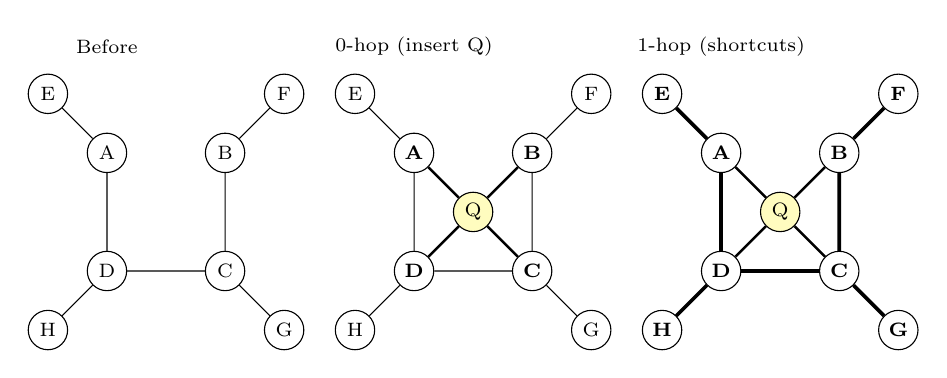
\begin{tikzpicture}[scale=0.75,
    node/.style={circle,draw,minimum size=5mm,inner sep=0pt, font=\scriptsize},
    lab/.style={font=\scriptsize}, pre/.style={font=\scriptsize,align=center}]
    % Left: Before (double square, no Q)
    \node[lab] at (0,2.8) {Before};
    \node[node] (A0) at (0,1) {A};
    \node[node] (B0) at (2,1) {B};
    \node[node] (C0) at (2,-1) {C};
    \node[node] (D0) at (0,-1) {D};
      % remove AB edge in Before
      \draw (B0)--(C0) (C0)--(D0) (D0)--(A0);
    \node[node] (E0) at (-1,2) {E};
    \node[node] (F0) at (3,2) {F};
    \node[node] (G0) at (3,-2) {G};
    \node[node] (H0) at (-1,-2) {H};
    % (outer ring edges removed for clarity)
    \draw (A0)--(E0) (B0)--(F0) (C0)--(G0) (D0)--(H0);

    % Middle: 0-hop insert Q
    \begin{scope}[xshift=5.2cm]
      \node[lab] at (0,2.8) {0-hop (insert Q)};
      \node[node, font=\scriptsize\bfseries] (A1) at (0,1) {A};
      \node[node, font=\scriptsize\bfseries] (B1) at (2,1) {B};
      \node[node, font=\scriptsize\bfseries] (C1) at (2,-1) {C};
      \node[node, font=\scriptsize\bfseries] (D1) at (0,-1) {D};
      % remove AB edge in 0-hop panel
      \draw (B1)--(C1) (C1)--(D1) (D1)--(A1);
      \node[node] (E1) at (-1,2) {E};
      \node[node] (F1) at (3,2) {F};
      \node[node] (G1) at (3,-2) {G};
      \node[node] (H1) at (-1,-2) {H};
      % (outer ring edges removed for clarity)
      \draw (A1)--(E1) (B1)--(F1) (C1)--(G1) (D1)--(H1);
      \node[node, fill=yellow!25] (Q1) at (1,0) {Q};
      \draw[line width=0.9pt] (Q1)--(A1) (Q1)--(B1) (Q1)--(C1) (Q1)--(D1);
      % stats moved to text bullets below to avoid overlap
    \end{scope}

    % Right: 1-hop shortcuts
    \begin{scope}[xshift=10.4cm]
      \node[lab] at (0,2.8) {1-hop (shortcuts)};
      \node[node, font=\scriptsize\bfseries] (A2) at (0,1) {A};
      \node[node, font=\scriptsize\bfseries] (B2) at (2,1) {B};
      \node[node, font=\scriptsize\bfseries] (C2) at (2,-1) {C};
      \node[node, font=\scriptsize\bfseries] (D2) at (0,-1) {D};
      % remove AB edge in 1-hop panel
      \draw (B2)--(C2) (C2)--(D2) (D2)--(A2);
      \node[node, font=\scriptsize\bfseries] (E2) at (-1,2) {E};
      \node[node, font=\scriptsize\bfseries] (F2) at (3,2) {F};
      \node[node, font=\scriptsize\bfseries] (G2) at (3,-2) {G};
      \node[node, font=\scriptsize\bfseries] (H2) at (-1,-2) {H};
      % (outer ring edges removed for clarity)
      \draw (A2)--(E2) (B2)--(F2) (C2)--(G2) (D2)--(H2);
      \node[node, fill=yellow!25] (Q2) at (1,0) {Q};
      \draw[line width=0.9pt] (Q2)--(A2) (Q2)--(B2) (Q2)--(C2) (Q2)--(D2);
      % Emphasize key edges
      % emphasize edges (without AB)
      \draw[line width=1.3pt] (B2)--(C2);
      \draw[line width=1.3pt] (C2)--(D2);
      \draw[line width=1.3pt] (D2)--(A2);
      \draw[line width=1.3pt] (A2)--(E2);
      \draw[line width=1.3pt] (B2)--(F2);
      \draw[line width=1.3pt] (D2)--(H2);
      \draw[line width=1.3pt] (C2)--(G2);
      % removed dashed evaluation arrows (評価は文中で定義)
      % stats moved to text bullets below to avoid overlap
    \end{scope}
  \end{tikzpicture}
  \vspace{0.6ex}
  \caption{二重正方形の最小例。左: 挿入前。中: 0-hop で Q を追加(曖昧さ増\,→\,Fは閾値上)。右: 1-hop で短絡が顕在化(到達性改善\,→\,F低下\,/DG へ)。補足: $\Delta H = H\big(Q\mid \{A,B,C,D\}\big) - H\big(Q\mid \{A,\dots,H\}\big) > 0$。}
  \label{fig:minimal_example}
\end{figure}

\begin{enumerate}
  \item \textbf{0-hop直後(中央図)}: 
  \begin{itemize}
    \item \textbf{評価対象(0-hop)}: ノード $\{\,Q,A,B,C,D\,\}$ とエッジ $\{\,Q\text{--}A,\;Q\text{--}B,\;Q\text{--}C,\;Q\text{--}D\,\}$ に限る。
    \item EPC: 5(ノード1+エッジ4追加)
    \begin{itemize}
      \item 局所正規化の分母: $C_{\max}(S_0)=c_{\mathrm{node}}+|S_0|\,c_{\mathrm{edge}}$ とし、単価を $c_{\mathrm{node}}{=}1,\ c_{\mathrm{edge}}{=}1$ とすれば $C_{\max}{=}1{+}4{=}5$。
      \item $\Delta\mathrm{EPC}_{\rm norm}{=}{5}/{5}{=}\mathbf{1.0}$。
    \end{itemize}
    \item IG($K{=}5$, $Z{=}\log 5$): $H_{\rm before}{=}\log 4{=}1.386$, $H_{\rm after}{=}\log 5{=}1.609$。$\Delta\mathrm{SP}{=}0$ として
      \[
        \Delta H_{\rm norm}\;=\;\frac{1.609-1.386}{\log 5}\;\approx\;\mathbf{+0.139}\quad(\gamma{=}0),\quad
        \Delta\mathrm{IG}_{\rm norm}\;=\;\Delta H_{\rm norm}\;\approx\;\mathbf{+0.139}.
      \]
    \item よって $\lambda{=}1$ で $g_0\;=\;1.0\; -\;0.139\;\approx\;\mathbf{0.861}$(AG発火)。
    \item → AG発火(探索継続)
  \end{itemize}
  \item \textbf{1-hop評価(右図)}:
  \begin{itemize}
    \item \textbf{評価対象(1-hop)}: 図に表記されている\,\emph{全ノード・全エッジ}($E,F,G,H$ から外部ノードへ伸びるエッジは評価対象外)。
    \item EPC(絶対): 0-hop と同一の挿入一式に対する絶対評価とし、$\Delta\mathrm{EPC}_{\rm norm}(1){=}\mathbf{1.0}$($C_{\max}$ は 0-hop と同値)。
    \item IG($K{=}9$, $Z{=}\log 9$): $H_{\rm before}{=}\log 8{=}2.079$, $H_{\rm after}{=}\log 9{=}2.197$。
      \[
        \Delta H_{\rm norm}\;=\;\frac{2.197-2.079}{\log 9}\;\approx\;\mathbf{+0.054}.
      \]
    \item SP(平均最短路長): 全ノードの全対平均で、\,\emph{Before}(左図)は $\mathrm{SPL}_{\rm before}=\tfrac{68}{28}{=}\mathbf{2.429}$、\,\emph{1-hop}(右図)は $\mathrm{SPL}_{\rm after}=\tfrac{76}{36}{=}\mathbf{2.111}$。
      \[
        \Delta\mathrm{SP}\;=\;2.111-2.429\;=\;-0.317,\qquad
        \Delta\mathrm{SP}_{\rm rel}\;=\;\frac{2.429-2.111}{\max\{2.429,\varepsilon\}}\;\approx\;\mathbf{0.131}.
      \]
      $\Rightarrow\;\Delta\mathrm{IG}_{\rm norm}\;=\;\Delta H_{\rm norm}+\gamma\,\Delta\mathrm{SP}_{\rm rel}\;\stackrel{\gamma=1}{\approx}\;\mathbf{0.054+0.131=0.185}$。
    \item よって $\lambda{=}1$ で $g^{(1)}\;=\;1.0\; -\;0.185\;\approx\;\mathbf{0.815}$。\;$g^{(1)}<g_0$(改善)。
  \end{itemize}
\end{enumerate}

\noindent 以上より、0\,\mbox{-}hop では統合可否が曖昧な知識を検知し、multi\,\mbox{-}hop では短絡と情報集中の両方を確認して、グラフの構造改善に資する知識かを判断できる。

% IG 数値例は上の箇条書きに統合済み

\paragraph{グラフ構造での同定制御}
この二段ゲートにより、知識グラフ上で以下の同定制御が可能になる:

\begin{table}[H]
\centering
\small
\begin{tabular}{llll}
\toprule
状態 & 0-hop ($g_0$) & Multi-hop ($g_{h}$) & 制御 \\
\midrule
明確な統合 & $g_0<\theta_{\mathrm{AG}}$ & - & 即座に受容 \\
曖昧な局面 & $g_0>\theta_{\mathrm{AG}}$ & 未評価 & AG 発火→探索深化 \\
真の洞察 & $g_0>\theta_{\mathrm{AG}}$ & $g_h<\theta_{\mathrm{DG}}$ & AG→統合確定 \\
擬似洞察 & $g_0>\theta_{\mathrm{AG}}$ & $g_h>\theta_{\mathrm{DG}}$ & 探索深化 \\
統合不要 & $g_0\gg\theta_{\mathrm{AG}}$ & $g_h\simeq\theta_{\mathrm{DG}}\ (h>H)$ & 棄却 \\
\bottomrule
\end{tabular}

\vspace{0.4ex}\noindent\footnotesize{注: $H$ は割り当て可能な計算リソース(時間/メモリ/問い合わせ枠など)により決定する。}\normalsize
\caption{0\,\mbox{-}hop と multi\,\mbox{-}hop の組み合わせによるグラフ構造の同定制御。5つの異なる状態を識別し、それぞれに適した制御を実行。}
\label{tab:graph_control}
\end{table}

この表が示すように、二つのシグナルの組み合わせにより、\textbf{5つの異なる状態を識別}し、それぞれに適した制御を実行できる。これが本手法の「One\,\mbox{-}Gauge 制御」の本質である。


\subsection{二段ゲート(AG/DG)の操作的対応}
\label{sec:ag_dg_gate}

本節は\,\emph{運用定義の要点のみ}を示す。理論上の対応は二重性(\S\ref{sec:dual_fep_mdl})とFEP–MDL命題(\S\ref{sec:fep_mdl_bridge})を参照。

\paragraph{ゲート定義}
\begin{equation}
  \mathrm{AG}(t) := \mathbb{I}[\, g_0(t) > \theta_{\mathrm{AG}}\,] \,.
  \label{eq:ag_trigger}
\end{equation}
\begin{equation}
  b(t) := \begin{cases}
    \min\{\, g_0(t),\; g_{\min}(t)\,\}, & \mathrm{AG}(t)=1\\
    g_0(t), & \mathrm{otherwise}
  \end{cases},\quad
  \mathrm{DG}(t) := \mathbb{I}[\, b(t) \le \theta_{\mathrm{DG}}\,] \,.
  \label{eq:dg_trigger}
\end{equation}

\noindent\textit{直観}\; AG は $\F$ が\,\emph{大きい}(曖昧な)局面で探索を促し、DG は multi\,\mbox{-}hop により $\F$ が\,\emph{小さくなった}(短絡で利得のある)局面で受容を確定する。

\paragraph{校正と運用}
\begin{itemize}[leftmargin=*]
  \item \textbf{閾値の校正}: $\theta_{\mathrm{AG}},\theta_{\mathrm{DG}}$ は分位ベースで適応(\S\ref{sec:hyperparam_drift}, \S\ref{sec:psz_calibration})。PSZ 制約下で FMR/P50 を監視しつつ運用(\S\ref{sec:equal_resources})。
  \item \textbf{AG 発火時の処理}: multi\,\mbox{-}hop 評価を強制し、必要に応じて $H/k$ を一時拡大(P95 ガードでクリップ)。
  \item \textbf{DG 判定時の処理}: 限界寄与に基づく\,\emph{接続コミット}(非寄与枝は採用しない)。手順は\S\ref{sec:event_driven_control}。
  \item \textbf{安定化の手当て}: 固定台正規化($C_{\max}$, $\log K$)、union/trim、距離キャッシュ、早期打ち切りを併用。
  \item \textbf{安全弁}: ロールバック用スナップショット、発火抑制(クールダウン)と履歴分位の併用。
  \item \textbf{計算予算との整合}: P95 遅延の予算内化(例: P95 $\le$ \SI{350}{ms})を優先し、$H\in\{1,2,3\}$、$k\in[8,64]$ から $O(k^H)$ を満たす\,\emph{最小構成}を選択。PSZ 制約下で運用し、FMR の上昇は許容しない。
  \item \textbf{クールダウン/バックオフ}: AG/DG の連続発火によるスラッシングを避けるため、再発火クールダウン(3--5 ステップ)と指数バックオフ(DG 失敗時は $k\downarrow/ H\downarrow$/ 一時的に $\theta_{\mathrm{AG}}\uparrow$)を導入。
\end{itemize}



\noindent 備考: 実装では AG フレーム上の $b(t)$ 分布に対する\textbf{下位分位}($q_\beta$)を用いて $\theta_{\mathrm{DG}}$ を自動適応させ、過検出と見逃しのトレードオフを制御する(\S\ref{sec:maze_experiment})。

\paragraph{安定受容サブグラフの観点}
AG–DG は、\emph{エピソードを安定的に受け入れられる局所サブグラフ}を探索・確定する過程としても解釈できる。受容判定の\emph{マージン}を $m(t):=\theta_{\mathrm{DG}}-b(t)$ とし、統合直前に\,\emph{小さな摂動(結び替え/しきい値ゆらぎ)}に対する再評価を少数回だけ行う\,\textbf{軽量監査}(\texttt{StabilityAudit})を挟む。\,$m(t)\ge \varepsilon$ が摂動下でも保たれるとき、DG を\,\emph{ロバスト受容}として確定し、疑似洞察の混入を抑える。

ここで $g_{\min}(t)$ は同一ステップにおける multi-hop geDIG の最小値である。multi-hop の負側(短絡)は\textbf{ループ閉鎖や経路短縮の検出}であり、価値予測的なドーパミン(DA)的信号に対応づけられる。

\noindent 注: 本稿では D-Gate を $\mathrm{DG}(t)$ と表記し、情報利得の $\Delta\mathrm{IG}$ と符号が衝突しないように区別する(\S\ref{sec:maze_experiment} でも同名を使用)。

\paragraph{操作的対応の解釈}
この AG/DG 対応は生理学的同定ではなく、\emph{operational correspondence}(操作的対応)として解釈されるべきである:
\begin{itemize}
  \item \textbf{AG的}: 不確実性検出 → 注意喚起 → 探索促進(FEP的誤差最小化)
  \item \textbf{DA的}: 短絡検出 → 価値評価 → 統合判断(MDL的複雑さ削減)
\end{itemize}

この二段ゲートにより、\textbf{曖昧さの検知と短絡の評価が同一ステップで連鎖}し、無駄探索を抑えつつ有益な橋構造の発見をリアルタイムにトリガする。


\paragraph{ハイパーパラメータ校正とドリフト対策}\label{sec:hyperparam_drift}
\textbf{目的}\; $\theta_{\mathrm{AG}},\theta_{\mathrm{DG}},\lambda,\,H,\,k$ を過度な手動調整に頼らず\,\emph{安定・再現可能}に運用する。
\begin{description}[leftmargin=1.6em]
  \item[閾値の分位校正] \; AG は $g_0$ の上位分位(例: $q_{1-\alpha}$)、DG は AG フレーム上の $b(t)$ の下位分位(例: $q_{\beta}$)で自動設定する:
  \[
    \theta_{\mathrm{AG}} \leftarrow q_{1-\alpha}\big(\{g_0\}_{t-W:t}\big),\qquad
    \theta_{\mathrm{DG}} \leftarrow q_{\beta}\big(\{b(t)\mid \mathrm{AG}(t){=}1\}_{t-W:t}\big).
  \]
  ウィンドウ長 $W$ は 1–5\,min(ストリーム)または 256–1024 ステップ(バッチ)の範囲で設定。指数移動分位(EWQ; 係数 $\rho\in[0.9,0.99]$)を用いて\,\emph{概念ドリフト}に追従させつつ過検出を抑制する。
  \item[スケール合わせ($\lambda$)] \; $\lambda$ は $\gednorm$ と $\ignorm$ の\,\emph{分散同規模化}で初期化する:
  \[
    \lambda_0 := \frac{\mathrm{Std}[\gednorm]}{\max\{\mathrm{Std}[\ignorm],\,\varepsilon\}}\,;\quad \lambda\in\{\tfrac{1}{2}\lambda_0,\lambda_0,2\lambda_0\}\ \text{でグリッド検証}.
  \]
  MDL 対応(\S\ref{sec:fep_mdl_bridge})を採る場合は $\lambda\approx c_D/c_M$ としてアンカーし、小規模グリッドで微調整する。
  \item[$\lambda$ の決定手順] \; 実務では次の手順で決定する:\,(1) パイロット $N{\approx}100$ で $\sigma_{\mathrm{EPC}}{=}\mathrm{Std}[\gednorm]$, $\sigma_{\mathrm{IG}}{=}\mathrm{Std}[\ignorm]$ を測定、\,(2) 初期値 $\lambda_0{=}\sigma_{\mathrm{EPC}}/\max\{\sigma_{\mathrm{IG}},\varepsilon\}$($\varepsilon{=}10^{-6}$)を設定、\,(3) グリッド $\{\tfrac{1}{2}\lambda_0,\lambda_0,2\lambda_0\}$ を比較、\,(4) PSZ 準拠率(Acc/FMR/P50)最大の $\lambda$ を選択、\,(5) 以後の全実験で固定(ドリフト防止)。この解釈は情報熱力学の温度($\beta{=}1/k_BT$)の離散系近似に対応する。
  \item[$\gamma$ の扱い] \; $\gamma$ は $\Delta H$ と $\Delta\mathrm{SP}_{\mathrm{rel}}$ の\,\emph{同次元内の配分係数}であり、既定は $\gamma\in\{0.0,0.5,1.0\}$ の\,\emph{低次元グリッド}で選ぶ。RAG では $\gamma{=}1.0$(経路短縮を情報側に全計上)を既定とし、迷路では $\gamma{\in}[0.5,1.0]$ を推奨。\,\emph{equal‑resources} 下で PSZや汚染率の感度を報告し、ドメイン変更時は\,\emph{初期グリッドのみ}を許容して固定する。
  \item[計算予算との整合] \; $H$ と $k$ は P95 遅延の\,\emph{予算内化}を優先する(例: P95 $\le$ \SI{350}{ms})。$H$ は 1–3、$k$ は 8–64 の範囲で、$O(k^H)$ を満たす最小構成を選ぶ。指標は PSZ(\S\ref{sec:psz_metrics})と併用し、FMR 上昇を許容しない。
  \item[クールダウンとバックオフ] \; AG/DG 連続発火によるスラッシングを防ぐため、\,\emph{再発火のクールダウン}(例: 3–5 ステップ)と、DG 失敗時の\,\emph{指数バックオフ}(候補幅縮小や $\beta\downarrow$)を導入する。
\end{description}

\paragraph{失敗様式と緩和策}\label{sec:failure_modes}
\begin{itemize}[leftmargin=*]
  \item \textbf{局所ループ/振動}($g_0$ が閾値近傍で振れる): EWQ による閾値平滑化、AG クールダウン、探索方針の多様化($\epsilon$-greedy で候補切替)。
  \item \textbf{誤統合(FMR 上昇)}: DG を下位分位で適応させつつ、受容直後は\,\emph{猶予期間のロールバック}(一定ステップ内の悪化で取り消し)。$\Delta\mathrm{SP}_{\mathrm{rel}}$ に\,\emph{重み付き負担}を加え橋の過剰形成を抑制。
  \item \textbf{過度な探索遅延}($H, k$ 過大): P95 監視で自動クリッピング($H\downarrow$ or $k\downarrow$)。$\theta_{\mathrm{AG}}\uparrow$ で発火頻度を抑制。
  \item \textbf{分布ドリフトによる閾値崩れ}: ウィンドウ更新と季節性(時間帯/ドメイン)別の分位テーブルを持つ。\,\emph{セッション頭のウォームアップ}中は固定閾値を使用。
\end{itemize}

\paragraph{反証可能な予測}
この設計は以下の反証可能な予測を与える:
\begin{enumerate}
  \item AG を無効化すると DA 評価が遅延し、無駄探索が増える
  \item Multi-hop を無効化すると短絡検出の質が下がり、バックトラックの精度が低下する
  \item $\theta_{\mathrm{AG}}$ を緩めすぎると過検出により計算コストが増大
  \item $\theta_{\mathrm{DG}}$ を厳しくしすぎると有益な統合を見逃す
\end{enumerate}

これらの予測は実験\S\ref{sec:maze_experiment}と\S\ref{sec:rag_experiment}で検証される。
\\[0.2em]
\noindent\textit{備考(Transformer 内在化)}\; 統一指標 $\F$ は、\,\textbf{層間推論における自由エネルギー型の評価量}としても読み替え可能である。注意グラフ上で $\Delta$EPC/$\Delta$IG を測定し、AG/DG を導入することで、内部計算においても\,\textbf{0\,\mbox{-}hop の誤差検知と multi\,\mbox{-}hop の最小化という工程分離}を実装設計に落とし込める。

\subsection{FEP–MDL ブリッジ(操作的命題;概要)}

\paragraph{操作的対応の定義}\label{para:operational_correspondence}
本稿における\emph{操作的対応(operational correspondence)}とは、以下の三条件を満たす関係を指す:(i)数理的同値ではなく\textbf{測定可能な量の比例関係}であること、(ii)仮定 (B1)–(B4) の下で\textbf{残差が $O(1/N)$ に評価}できること、(iii)\textbf{実験で検証可能な予測}(方向付け)を与えること。具体的には、FEP の自由エネルギー(予測誤差+複雑性)と geDIG の単一ゲージ $\F=\gednorm-\lambda\ignorm$ を
\begin{itemize}[leftmargin=1.2em]
  \item 0\,\mbox{-}hop \,$\leftrightarrow$\, 誤差/曖昧さの検出(FEP)
  \item multi\,\mbox{-}hop \,$\leftrightarrow$\, 複雑さの圧縮(MDL)
\end{itemize}
という\,\textbf{操作的対応}として扱い、仮定 (B1)–(B4) の下で
\begin{equation*}
  \F\;\propto\; \Delta\mathrm{MDL}\; +\; O(1/N)
\end{equation*}
が成り立つ(比例係数は $\lambda\approx c_{\!D}/c_{\!M}$:MDL の項比)。本節は詳細証明ではなく、以降の実験章で検証する\,\textbf{運用上の予測可能性}を与えるための定義づけである。

\paragraph{読み方ガイド(何を主張し、何をしないか)}
FEP–MDL ブリッジは、「$\F$ がどのような意味で自由エネルギー/MDL と整合しているか」を\,\textbf{操作的に整理するための節}であり、完全な理論同値や厳密な最適性を主張するものではない。
読者は、(i) $\F$ が $\Delta\mathrm{MDL}$ に比例するという命題は(仮定付きの)\emph{設計上の指針}であり、(ii) 実験で検証するのは「ゲージ設計の方向付けが妥当かどうか」であって、FEP 全体の真偽ではない、という二点を念頭に置いて読めばよい。
より実装寄りに読む場合は、本節を「なぜ構造項と情報項をこの分離で採ったのか」という\emph{設計理由のメモ}として理解し、詳細な変分推論の議論は付録と今後の理論研究に委ねてよい。
\begin{comment}
ここでは、0\,\mbox{-}hop/multi\,\mbox{-}hop の二重性と二段ゲート(AG/DG)が\,\textbf{FEP(自由エネルギー原理)とMDL(最小記述長)の対応}として\,\emph{操作的に整合}することだけを要点として述べる。すなわち、正規化・上界・比例吸収の仮定(B1–B4)の下で、
\[\;\F\ \propto\ \Delta\mathrm{MDL}\;\]
が\,\emph{残差 $O(1/N)$ を除いて成立}する、という\,\textbf{運用上の命題}である。

\noindent \textbf{仮定(B1)–(B4)}:
\begin{description}[leftmargin=1.8em]
  \item[(B1) 局所有界性] 編集コストは $C_{\max}$ で上界化され、評価する multi-hop のホライズン $H$ は有限である。
  \item[(B2) 編集分解] 置換操作は削除+挿入の和で上界近似でき、\,\textbf{編集経路コスト(EPC)}を加法的な編集操作の総和として表せる。
  \item[(B3) エントロピー推定] 局所エントロピー差分の推定誤差分散は $\sigma_H^2=O(1/|\mathcal{N}|)$ と評価できる(一様収束する推定量を使用)。
  \item[(B4) 正規化安定性] $C_{\max}(S_h)$ は $|S_h| \le K_{\max}(\theta_{\mathrm{sim}},k)$ によって有界で、エントロピー項の正規化分母は $\log K$ を用いる($K$ はサブグラフ $S_h$ のノード数)。
\end{description}
\noindent なお、(B1)–(B3)は 3.5 節の\,\emph{埋め込み空間 $\Phi$ の要件}(A1: 意味的勾配、A2: ノルム正規化、A3: 局所的滑らかさ)により実務上満たされる仮定である。

\paragraph{単位と換算(U1–U3)}
\begin{description}[leftmargin=1.8em]
  \item[(U1) 編集単価の符号化上界] 1 回の編集操作(種別+対象ID+局所メタ)は高々 $\alpha$\,bits のプレフィックス符号で上界化できる(定数 $\alpha>0$)。
  \item[(U2) 問い合わせ単価の換算] 1 hop の参照/問い合わせは平均 $\kappa$\,bits の情報量に相当する(定数 $\kappa>0$)。
  \item[(U3) 比率の解釈] 比例係数は $\lambda\approx c_{\mathrm{ig}}/c_{\mathrm{ged}}\approx \kappa/\alpha$ として尺度合わせを解釈し、$\gamma$ は\,\emph{hops→bits} の換算係数として $\Delta\mathrm{SP}_{\mathrm{rel}}$ を情報側($\ignorm$)に計上する。
\end{description}
\noindent 注: $\alpha,\kappa$ は局所定常(観測窓内で一定)を仮定する。非定常/無界に変動する場合は\,\S\ref{sec:fep_mdl_bridge_applicability} の適用範囲の注意に従う。

\begin{lemma}[構造符号長の上界化]
\label{lem:structure_code_length_old}
仮定 (B1)・(B2) の下で、$h$-hop 誘導部分グラフ $G'_h$ の構造符号長差分 $\Delta L_M:=L(M_{\mathrm{after}})-L(M_{\mathrm{before}})$ は
\[
  \Delta L_M \;\le\; c_{\mathrm{ged}}\,\gednorm + O(1/N)
\]
を満たす定数 $c_{\mathrm{ged}}>0$ が存在する。ここで $N$ は評価対象グラフのノード数である。
\end{lemma}

\noindent\textit{注}: ここでの $N$ は $N:=|G'_h|$(評価対象の誘導部分グラフのノード数)を指す。正規化上界 $C_{\max}$ は $S_{\mathrm{link}}$ 起点で固定されているため、分母の変動は残差に吸収される((B4))。

\begin{proof}[証明の概略]
編集操作(挿入・削除)の単価をプレフィックス符号で $c_{\mathrm{ins}}, c_{\mathrm{del}}$ と定め、$C_{\max}$ を (A1) に従って $h$-hop 部分グラフで発生し得る最大コストとする。置換操作は (A2) により削除+挿入に分解でき、構造符号長差分は $\sum_i c_{\mathrm{edit}}^{(i)}$ で上界化される。正規化により $C_{\max}\gednorm$ がこの総和の上界となり、有限ホライズンでの境界効果は $O(1/N)$ に吸収される。
\end{proof}

\begin{lemma}[データ符号長の収束]
\label{lem:data_code_length_old}
仮定 (B1)・(B3) の下で、局所エントロピー差分に基づくデータ符号長 $\Delta L_D:=L(D\mid M_{\mathrm{after}})-L(D\mid M_{\mathrm{before}})$ は
\[
  \Delta L_D \;=\; -\,c_{\mathrm{ig}}\,\ignorm + O(1/N)
\]
を満たす定数 $c_{\mathrm{ig}}>0$ が存在する。
\end{lemma}

\paragraph{理論から実装へ(アルゴリズムへの橋渡し)}
以上の定義・仮定に基づく\,\textbf{統一ゲージのイベント駆動制御}(観測→$\Delta$EPC/$\Delta$IG→$g_0/g_{\min}$→AG/DG 判定→探索/受容)の手順は、次章の制御節(§\ref{sec:event_driven_control})に擬似コード(Algorithm\,1)としてまとめる。理論量($\gednorm,\ignorm,\,g_0,\,g_{\min}$)は、そこに示す逐次手順で実時間に近い形で算出・判定される。

\begin{proof}[証明の概略]
局所分布 $p$ に対する符号長は $-\sum_j p_j\log p_j$ に収束し、(A3) により推定誤差の分散は $O(1/|\mathcal{N}|)$ で抑制される。正規化 $\ignorm$ により $H_{\text{before}}-H_{\text{after}}$ が $\Delta L_D$ の主成分を与え、残差は有限標本および正規化定数の微小変動として $O(1/N)$ に吸収される。
\end{proof}

\noindent 本命題は $h{=}0$ の即時評価を対象とし、multi-hop ($h\ge1$) における短絡利得は \eqref{eq:ignorm_main} の $\gamma\,\Delta\mathrm{SP}_{\mathrm{rel}}$ として情報利得側に含めて扱う(後述の系を参照)。

\begin{proposition}[運用MDL命題]
仮定 (B1)〜(B4) の下で正の定数 $c_{\mathrm{ged}}, c_{\mathrm{ig}}$ が存在し、
\[
  \Delta L = c_{\mathrm{ged}}\,\gednorm - c_{\mathrm{ig}}\,\ignorm + \varepsilon
\]
が成り立つ。ここで $\Delta L$ は記述長の変化であり、残差は $|\varepsilon|\le O(1/N)$。比例係数を $\lambda=c_{\mathrm{ig}}/c_{\mathrm{ged}}$ と選べば、$\F=\gednorm-\lambda\,\ignorm$ は $\Delta\mathrm{MDL}$ に比例する。
\end{proposition}

\begin{proof}[証明の概略]
MDL は $L(M)+L(D\mid M)$ に分解できる。構造項は補題\ref{lem:structure_code_length}より $c_{\mathrm{ged}}\gednorm+O(1/N)$ に上界化され、データ項は補題\ref{lem:data_code_length}より $-c_{\mathrm{ig}}\ignorm+O(1/N)$ に収束する。(B4) により正規化定数(分母 $\log K$)の変動も残差に吸収できるため、両者の和を取れば主項が命題の式を与える。比例係数 $\lambda=c_{\mathrm{ig}}/c_{\mathrm{ged}}$ を採用すれば $\F$ は $\Delta\mathrm{MDL}$ に比例すると結論づけられる。
\end{proof}

\paragraph{二部記述長の上界構成(達成可能性)}
\label{sec:two_part_achievability}
\emph{構成(スケッチ)}: モデル符号 $L(M)$ は編集列を操作種別+対象IDのプレフィックス符号で表し、各操作の符号長を $\le\alpha$ bits に抑える((U1))。よって構造差分は
\(\Delta L_M\le \alpha\cdot C_{\mathrm{edit}}(G_{\mathrm{before}}\rightarrow G_{\mathrm{after}})+O(1)\),
正規化により $\propto \gednorm$ の上界となる。データ符号 $L(D\mid M)$ は局所分布に基づく算術符号で与え、\,$\Delta L_D\approx -c_{\mathrm{ig}}\,(\Delta H_{\mathrm{norm}}+\gamma\,\Delta \mathrm{SP}_{\mathrm{rel}})$\,と読める($\Delta \mathrm{SP}$ は 1 hop$\approx\kappa$\,bits の通信削減として情報側に計上;(U2)–(U3))。以上より、二部記述長の\,\emph{達成可能な上界}として命題の主張を満たす。

\paragraph{適用範囲と限界}\label{sec:fep_mdl_bridge_applicability}
操作語彙が無限に増殖する、あるいは $\alpha,\kappa$ が非定常/無界に変動する設定では、上記の MDL 読み替えは成立しない。その場合、本指標 $\F$ は\,\emph{運用コストの近似ゲージ}として解釈し、MDL 整合は適用外とする。

\paragraph{熱力学的対応(比喩)}
Helmholtz の自由エネルギー $\Delta F = \Delta U - T\,\Delta S$ に\,\emph{操作的な比喩}を与える。いま本稿の定義より
\[
  \F\;=\;\Delta\mathrm{EPC}_{\mathrm{norm}}\; -\; \lambda\,\big(\,\Delta H_{\mathrm{norm}} + \gamma\,\Delta \mathrm{SP}_{\mathrm{rel}}\,\big)
  \,=\;\underbrace{\big(\Delta\mathrm{EPC}_{\mathrm{norm}} - \lambda\,\gamma\,\Delta \mathrm{SP}_{\mathrm{rel}}\big)}_{\text{\small 構造コストの有効項}}\; -\; \underbrace{\lambda\,\Delta H_{\mathrm{norm}}}_{\text{\small エントロピー項($\propto\,\Delta S$)}}\,.
\]
この分解に従えば、\,\emph{内部エネルギー}(複雑性)$\Delta U$ に対応するのは $\Delta\mathrm{EPC}_{\mathrm{norm}} - \lambda\,\gamma\,\Delta \mathrm{SP}_{\mathrm{rel}}$(短絡による構造効率の向上を織り込んだ\,"有効な構造コスト")であり、\,\emph{エントロピーの変化} $\Delta S:=H_{\mathrm{after}}-H_{\mathrm{before}}$ に対しては $\Delta H_{\mathrm{norm}}\propto \Delta S$ と読む。係数 $\lambda$ は $kT$ に相当し、$\F\approx \Delta U - T\,\Delta S$ の\,\emph{操作的な比喩}として扱う。

いずれにせよ、\,\emph{構造コスト(内部エネルギー)}と\,\emph{エントロピー項}のトレードオフを単一スカラーで制御するというFEPの基本原理にヒューリスティックに一致する——短期(0‑hop)では $\lambda\,\Delta H_{\mathrm{norm}}$ による\,\emph{驚き最小化}、長期(multi‑hop)では $\Delta\mathrm{SP}_{\mathrm{rel}}$ を通じた\,\emph{構造効率の向上}が同じ $\F$ の枠内で両立する。

\paragraph{工程分離としてのFEP運用(0\,\mbox{-}hop検知 \texorpdfstring{$\rightarrow$}{->} multi\,\mbox{-}hop最小化)}
従来のFEPは「予測誤差の最小化」を\,\emph{単一の変分目的}に畳み込み、一括で最適化する実装が多い。geDIGはこれを\,\textbf{工程分離}し、(i) 0-hopでの\,\emph{安価な誤差検知}と、(ii) 必要時のみ実行する\,\emph{multi-hopでの誤差/複雑さ最小化}に分ける。具体的には、式\eqref{eq:F_job_evidence_intro}, \eqref{eq:ignorm_main} に基づき
\(g_0=\Delta\mathrm{EPC}_{\mathrm{norm}}-\lambda\,\Delta H_{\mathrm{norm}}\) を前段で評価し、$g_0>\theta_{\mathrm{AG}}$ のときだけ
\(g_{\min}=\min_{1\le h\le H}\{\Delta\mathrm{EPC}_{\mathrm{norm}}-\lambda(\Delta H_{\mathrm{norm}}+\gamma\,\Delta\mathrm{SP}_{\mathrm{rel}}^{(h)})\}\)
を後段で評価して、$b(t)=\min\{g_0,g_{\min}\}\le\theta_{\mathrm{DG}}$ の場合に統合をコミットする(\S\ref{sec:ag_dg_gate})。この工程分離により:
\begin{itemize}[leftmargin=*]
  \item \textbf{anytime性}: 安価な前段/高価な後段の二段実行で予算に適合し、中断可能な運用ができる
  \item \textbf{自動スロットリング}: 分位ベースのAG/DG(式\ref{eq:ag_trigger},\ref{eq:dg_trigger})で過検出/見逃しを制御
  \item \textbf{可観測性}: $g_0/g_{\min}$ 分布や発火率を計器化でき、巨大な一回最適化よりデバッグ容易
  \item \textbf{役割分担}: 0\,\mbox{-}hop=FEP的誤差検知、multi\,\mbox{-}hop=MDL的圧縮という二重性(\S\ref{sec:dual_fep_mdl})を運用可能に落とし込む
  \item \textbf{制約適合}: 枝コミット時に離散制約(次数/疎性/資源)やロールバック規則を一括適用しやすい
\end{itemize}
以上をもって、本稿の優位点は「自由エネルギー最小化の\,\emph{工程分離}」を単一ゲージ $\F$ と二段ゲート(AG/DG)で実務化した点にあると位置づけられる。

なお、この対応は\,\emph{比喩}であり物理的同一性を主張しない。$\lambda$ は\,\emph{情報温度}としての尺度合わせ係数であり、$\F$ は\,\emph{尺度合わせとトレードオフ構造}を説明する操作的な自由エネルギーの読み替えである。

\paragraph{FEP--MDL 対応(要約)}
以上の仮定 (B1)--(B4) により、構造符号長とデータ符号長の変化は $\\gednorm$ と $\\ignorm$ に比例し、記述長の変化 $\\Delta L$ は
\\[
  \\Delta L \\approx c_{\\mathrm{ged}}\\,\\gednorm - c_{\\mathrm{ig}}\\,\\ignorm
\\]
と読める。比例係数 $\\lambda\\approx c_{\\mathrm{ig}}/c_{\\mathrm{ged}}$ を採用すれば、$\\F=\\gednorm-\\lambda\\ignorm$ は記述長変化 $\\Delta\\mathrm{MDL}$ に\\emph{比例する運用ゲージ}として解釈できる。より厳密な補題・証明スケッチや Helmholtz 自由エネルギーとの比喩的対応は、後半の FEP--MDL 節(\\S\\ref{sec:fep_mdl_bridge})にまとめる。本節の理解に FEP/MDL の専門的な知識は必要なく、「構造コストと情報利得のトレードオフが MDL 的な圧縮原理と整合する」という程度の直観を持っておけば十分である。

MDL/FEP と本指標 $\\F$ の対応を表\\,\\ref{tab:theory_mapping_summary} に整理する(詳細は本文参照)。

\begin{table}[H]
\centering
\small
\resizebox{\textwidth}{!}{%
\begin{tabular}{@{}p{0.20\linewidth}p{0.26\linewidth}p{0.26\linewidth}p{0.26\linewidth}@{}}
\toprule
枠組み & 構造的コスト成分 & 情報/精度成分 & 目的(トレードオフ) \\
\midrule
最小記述長(MDL) & モデル記述長の増分 & データ記述長の減分 & 総記述長の最小化 \\
自由エネルギー(FEP) & 複雑性(事前/内部エネルギー) & 精度/驚き低減(エントロピー項) & 自由エネルギーの最小化 \\
\textbf{本稿指標 $\F$} & $\Delta\mathrm{EPC}_{\mathrm{norm}}\; -\; \lambda\gamma\,\Delta\mathrm{SP}_{\mathrm{rel}}$ & $\Delta H_{\mathrm{norm}}$ & $\F=\Delta\mathrm{EPC}_{\mathrm{norm}}-\lambda\,\big(\Delta H_{\mathrm{norm}}+\gamma\,\Delta\mathrm{SP}_{\mathrm{rel}}\big)$ の低減 \\
\bottomrule
\end{tabular}}
\caption{理論枠組みの対応表。$\lambda$ は情報温度($kT$)に相当する尺度合わせ係数として解釈する。}
\label{tab:theory_mapping_summary}
\end{table}

\section{イベント駆動制御の仕組み}
\label{sec:event_driven_control}

\subsection{制御アルゴリズム}
洞察イベント($b(t)\le\theta_{\mathrm{DG}}$)の検出をトリガに、探索方略・候補分岐・バックトラック・記憶エビクションを \textbf{単一基準} で制御する。
\\
\noindent\textbf{アルゴリズムの流れ(要約)}\; まず新規エピソード $e_t$ を\,\emph{仮に統合}して $g_0{=}\Delta\mathrm{EPC}_{\rm norm}{-}\lambda\,\Delta\mathrm{IG}_{\rm norm}$ を計算し、\,\textbf{AG}(曖昧検知)を判定する。必要に応じて $h{\ge}1$ の\,\emph{multi\,\mbox{-}hop} を展開し、各 $F^{(h)}$ を比較して \,$g_{\min}{=}\min_h F^{(h)}$ を得る。最後に $\min\{g_0,g_{\min}\}\le\theta_{\rm DG}$ なら\,\textbf{DG}(受容)を確定し、統合・枝刈り・バックトラック・メモリエビクションを実施する。\,\emph{しきい値 $\theta_{\rm AG},\theta_{\rm DG}$ は分位校正に基づく}(§\ref{sec:eval_protocol}, §\ref{sec:hyperparam_drift})。以下に擬似コードを示す(Algorithm~\ref{alg:one_gauge})。

\begin{algorithm}[H]
\caption{One\,\mbox{-}Gauge イベント駆動制御}\label{alg:one_gauge}
\begin{algorithmic}[1]
\State 観測 $o_t$ から新エピソード $e_t$ 生成
\State $\Delta G \gets \textsc{NormalizedEPC}(G_{t-1}, G_t)$ \Comment{$\Delta G = \Delta\mathrm{EPC}_{\mathrm{norm}}$}
\State $\Delta I \gets \textsc{EntropyIG}(X_{t-1}, X_t)$
\State $g_0 \gets \Delta G - \lambda\,\Delta I$
\State $g_{\min} \gets \min_{h=1}^{H}\, \textsc{MultiHop}(h)$
\State $b(t) \gets \min\{g_0, g_{\min}\}$;\; $m(t) \gets \theta_{\mathrm{DG}}-b(t)$
\If{$g_0 > \theta_{\mathrm{AG}}$}
  \State \textsc{NoveltyAlert}() \Comment{探索深化}
\EndIf
\If{$b(t) \le \theta_{\mathrm{DG}}$ \textbf{and} \textsc{StabilityAudit}($m(t)$, jitters)$\ge \varepsilon$}
  \State \textsc{BacktrackOrPrune}() \Comment{枝刈り・再配線}
  \State \Comment{Check $\Delta \mathrm{SP}$(擬似短絡抑制)}
  \State \textsc{AcceptAndIntegrate}($e_t$);\; \textsc{MemoryEviction}() \Comment{統合と必要に応じたエビクション}
\EndIf
\end{algorithmic}
\end{algorithm}

\paragraph{0-hopとmulti-hopの直感的な読み方}
0\,\mbox{-}hop 評価 $g_0$ は、新しい枝(エピソード接続)を仮に繋いだ「その場」で、\emph{ごく近傍だけ}を見て悪化していないかを判定する\,\emph{局所チェック}である。迷路の比喩では「1手だけ進んで、すぐ行き止まりに向かっていないか」を見る段階に相当する。一方 multi\,\mbox{-}hop 評価 $g_{\min}$ は、その枝を数ステップ先まで辿ったときに\,\emph{本当にショートカットになっているか}(平均最短路長が縮んでいるか)を判定する\,\emph{経路チェック}である。RAG に写像すると、0\,\mbox{-}hop は新規ノード周辺の\textbf{局所構造悪化の即時検知}、multi\,\mbox{-}hop はそのノード経由の\textbf{多ホップ経路が実際に役立つかの確認}と解釈できる。AG は前者(局所悪化の検知)に、DG は後者(ショートカット確認と統合確定)に対応する。

\paragraph{一般化可能性}\; 擬似コード中の環境依存な条件(例: 迷路での壁判定)は\,\emph{前処理/表現層}に留め、受容/探索/剪定の\,\textbf{判定基準そのものは $\F$ と AG/DG の規約で共通化}する。表現設計を差し替えれば、他ドメイン(RAG など)にも同一の制御原理を適用できる。

\subsection{実装ガイダンス(Phase~1)}
\noindent\textit{パラメータ $\lambda,\gamma$ の設定}\; 構造項と情報項のスケール合わせとしての $\lambda$ は、「備考: IG の近似性と $\lambda$ の解釈」で述べたように、まず分散同規模化による初期値 $\lambda_0:=\mathrm{Std}[\gednorm]/\max\{\mathrm{Std}[\ignorm],\varepsilon\}$ を求め、小さなグリッド $\{\tfrac{1}{2}\lambda_0,\lambda_0,2\lambda_0\}$ で PSZ 達成率と FMR/遅延を観察する。
実運用では、一度決めた $\lambda$ をシステム全体で固定し、環境ごとに頻繁にチューニングしない(図\ref{fig:psz_operating_curves_lite_ja} および付録の $(\tau,\lambda)$ Operating Curves を参照)。$\gamma$ は $\Delta H$ と $\Delta\mathrm{SP}_{\rm rel}$ の寄与バランスを決める係数であり、迷路PoCでは $\gamma{\approx}0.5$ 前後の範囲で感度が低いことを確認している。
\\
\noindent\textit{類似度計算と Linkset 構成}\; 実装では、エピソード埋め込み $\phi(e)\in\mathbb{R}^d$ に対し、重み付きコサイン類似度に基づく Top-$k$ 取得で $S_{\mathrm{link}}$ を構成する(重みはタスク別の重みベクトル管理で付与; コード例: \texttt{src/insightspike/search/similarity\_search.py})。
検索時には C-value を使わず純粋な類似度のみで順位付けし、$\F$ と AG/DG はその上に載る「統合ゲージ」として用いる。
これにより、既存のベクトルDBや ANN インデックスと容易に接続できる。
\\
\noindent\textit{バックトラックとエビクション}\; PoC 実装では、DG 発火時に「どこまで戻るか」は BFS/最短路に基づくグラフ上の分岐点復元で行い、受容済み/保留ノードの信頼度 $c_{\mathrm{confirmed}},c_{\mathrm{pending}}$ に応じて\emph{容量制約付きのエビクション}(低信頼かつ古いエピソードから優先的に削除)を行う。
一般化された実装では、(i) バックトラックは「$\F$ が悪化し始めた直前のステップ」まで巻き戻す、(ii) エビクションは「AG/DG ログを参照した LRU+低信頼度」規則で行う、という二段方針を採用すればよい。
計算量の概算とボトルネックは表\ref{tab:complexity_summary} に整理しており、$H,k,M$ をこの表を見ながら P50/P95 遅延とトレードオフさせるのが安全な運用設計となる。

% 反証可能な予測(重複セクション)は\S\ref{sec:ag_dg_gate} 内の段落に統合

\section{Proof of Concept: 部分観測迷路での統一指標制御}
\label{sec:maze_experiment}

\subsection*{結果サマリ(Maze;結果先行)}
\label{sec:maze_result_summary}
本節の主目的は、\textbf{未知迷路における探索効率の改善}を定量化することである。参照(Dijkstra/A*)は\,\emph{理想上限}として整合度(Regret/SPL や順位相関)で扱う\footnote{Regret はオラクル(最短路)との差の累積。SPL(Success weighted by Path Length)は成功時の効率(実行経路長と最短経路長の比)を表す。}。代表結果(25\,\mbox{$\times$}\,25, \,$N{=}32$;L3\,only, max\,steps=250)の要点を先にまとめる:
\begin{itemize}[leftmargin=1.4em]
  \item \textbf{探索率}(unique/total): 25.6\%(全シード平均;25\,\mbox{$\times$}\,25; eval 系列)
  \item \textbf{訪問重複率}: 平均 1.33 回/訪問セル(全シード平均;25\,\mbox{$\times$}\,25; eval 系列)
  \item \textbf{平均バックトラック長}: 近似 1.0 ステップ(dead\,\mbox{-}end 連続長の近似; 全シード平均;eval 系列)
  \item \textbf{デッドエンド検出遅延}: 平均 0 ステップ($\approx$ 即時;全シード平均;eval 系列)
  \item \textbf{成功率}: 56.3\%(25\,\mbox{$\times$}\,25, \,$N{=}32$;max\,steps=250)/ 98.0\%(15\,\mbox{$\times$}\,15, \,$N{=}100$)
  \item \textbf{参照近接}: Regret(最短路との差)と SPL を上限参照として併記し、Frontier 優先度との順位相関 $\rho$ で「Dijkstra 的な探索順序」にどれだけ近づいているかを確認した(geDIG の $-F$ と Dijkstra 優先度の整合性)。
\end{itemize}

\paragraph{設計要素と結果の対応}\; (1) \textbf{統一指標制御}の有効性は、対照($\Delta$EPC\,only/$\Delta$IG\,only)よりも良好な総合指標(成功率/ステップ/圧縮率)で示される(表~\ref{tab:maze_v4_main})。(2) \textbf{二段ゲート}の適切性は、0\,\mbox{-}hop と 1\,\mbox{-}hop の役割分担(図~\ref{fig:minimal_example})と発火統計(DG/AG 比率)の安定から確認できる。 (3) \textbf{クエリ中心 multi\,\mbox{-}hop} の効率は、$H\in\{1,2,3\}$ の軽量設定で短絡検出と計算量のバランスが取れる点(§\ref{sec:graph_model_premise} のコスト見積もり)に表れる。
\noindent 以上は、\textbf{$g_0$ による停滞の即時検知}と\,\textbf{DG による最近傍未探索分岐への復帰}が、\,\emph{無駄歩きの最小化}に直結していることを示す(仕組みの要点は \S\ref{sec:ag_dg_gate})。詳細統計・図表は補遺を参照(Regret 箱ひげ・訪問ヒートマップ・BT 軌跡・Frontier 散布)。

\begin{figure}[H]
  \centering
  \IfFileExists{figures/fig5_maze_scaling.pdf}{%
    \includegraphics[width=.74\linewidth]{figures/fig5_maze_scaling.pdf}%
  }{%
    \IfFileExists{figures/fig5_maze_scaling.tikz.tex}{\input{figures/fig5_maze_scaling.tikz.tex}}{\fbox{\parbox{0.72\linewidth}{\centering 図準備中(fig5\_maze\_scaling)}}}%
  }
  \caption{迷路スケーリング(L3; seeds=100/32/40, steps=250): 成功率(左軸, 青)と平均ステップ数(右軸, 赤)のサイズ依存。15\,\mbox{$\times$}\,15で高成功率/短ステップ、25\,\mbox{$\times$}\,25で歩留まり低下、51\,\mbox{$\times$}\,51では成功率が飽和前(探索予算不足)。}
  \label{fig:maze_scaling}
\end{figure}

本章では、部分観測迷路環境において、動的知識グラフが i) 新規エピソードを\textbf{受容/保留/棄却}する選別判断と、ii) 記憶(エピソードグラフ)を\textbf{探索・再利用}する行動選好を、\textbf{同一の計器 $\F$ と二段ゲート(AG/DG)で同居}させられるかを原理検証(Proof of Concept)する。最小構成(8次元状態ベクトル、部分観測、逐次グラフ配線)において、以下の設計要素が一体として動作することを示す:

\begin{enumerate}
\item \textbf{統一指標制御}:$\Delta$EPC と $\Delta$IG を統合した単一スカラー $\F$ により、\textbf{新規エピソードの選別(受容/保留/棄却)と探索方策}をイベント駆動で決定
  \item \textbf{二段ゲート(AG/DG)}:0\,\mbox{-}hop(Novelty)で停滞/曖昧を検出し、multi\,\mbox{-}hop(Backtrack/統合)で\textbf{ショートカット検証→受容}を実行
  \item \textbf{クエリ中心マルチホップ評価}:局所的クエリ起点の k-hop 部分グラフ評価により\textbf{スケーラブルな EPC 評価}を行い、探索と選別の同居を支える
\end{enumerate}

\paragraph{原理検証としての位置づけ}
本章は\textbf{探索効率}の検証を主眼とする\,\emph{PoC} であり、Dijkstra/A* は\,\emph{理想上限の参照枠}として扱う。\textbf{RAG そのものの性能評価ではなく}、\textbf{学習(エピソード統合)と推論(探索/バックトラック)を同時進行させる世界モデル更新ループ}が、完全に制御可能な環境で期待どおり動作するかを確かめるための最小実装である。確認対象は:(i)$\F{=}\Delta\mathrm{EPC}_{\mathrm{norm}}{-}\lambda\,\Delta\mathrm{IG}$ の\,\emph{実時間計算}、(ii)\,\emph{二段ゲート}(0\,\mbox{-}hop: 停滞検知, multi\,\mbox{-}hop: 短絡確認)の\,\emph{設計通りの挙動}、(iii)\,\emph{クエリ中心 multi\,\mbox{-}hop} による\,\emph{計算量と精度の管理}、の3点である(詳細アルゴリズムは付録参照)。

\noindent 重要な限定: 迷路におけるエピソード表現(式\ref{eq:state_vec})・クエリ(式\ref{eq:query_vec})・重み(式\ref{eq:weights_vec})は\textbf{迷路ドメインに特化}した設計である。他ドメイン(RAGなど)では表現設計が異なるが、\emph{統一ゲージによる評価・制御}($\F$と2段階ゲート)は\textbf{同じ原理}で運用できることを次章で示す。

\subsection{実験設計}
\begin{figure}[H]
  \centering
  \includegraphics[width=.82\linewidth]{fig4_maze.pdf}
  \caption{迷路PoCの概観(例: 25\,$\times$\,25)。スタート/ゴール、到達経路、観測候補、クエリ\,\mbox{-}hub による暫定配線を模式的に示す。本文の geDIG 評価は、0\,\mbox{-}hop の Top\,L 暫定配線(S\_link)と multi\,\mbox{-}hop の段階評価($g(h)$)を組み合わせ、AG/DG 二段ゲートでコミット/保留を制御する。}
  \label{fig:maze_overview}
\end{figure}

\paragraph{評価指標と成功基準(Maze)}\label{sec:maze_metrics_success}
\textbf{Primary(探索効率)}: \;探索率(\,unique\,/\,total\,), 訪問重複率(\,steps\,/\,unique\,), 平均バックトラック長(AG\,$\to$\,DG), デッドエンド検出遅延(deadend\,$\to$\,AG), 成功率。\\
\textbf{Secondary(参照近接)}: \;Regret $=$ steps$-L^*$(\,小さいほど良い\,), \;SPL $=L^*/\max\{L^*,\,\text{steps}\}$(\,1に近いほど良い\,)。\\
\textbf{診断}(付記): \;P50/P95 時間、AG/DG 発火率、Frontier 順位相関(geDIG の $-F$ と Dijkstra 優先度)、経路一致度(Jaccard)。\\
\textbf{成功基準の例(25\,\mbox{$\times$}\,25)}: \;探索率 $\le 0.40$, \;訪問重複 $\le 1.5$, \;BT 長 $\le 5$, \;検出遅延 $\le 1$, \;成功率 $\ge 95\%$, \;Regret 中央 $\le +3$, \;SPL 平均 $\ge 0.90$。(15/50 は規模別で設定)

\subsection{成功基準(定量的)}\label{sec:maze_success_criteria}
\textbf{Layer 1: 必要条件(原理動作)}.\; 成功率$\ge95\%$(25\,\mbox{$\times$}\,25, $N{=}100$)、AG発火率5--10\%、DG発火率2--5\%、DG/AG比30--50\%、閾値安定性(訓練/検証の発火率差$\le2$\%)。\\
\textbf{Layer 2: 十分条件(効率性)}.\; 探索率$\le0.40$、訪問重複$\le1.5$、BT長$\le5$、検出遅延$\le1$、Greedy\,Novelty比で有意(Welch, Bonferroni, $p{<}0.01$, Cohen's $d{>}0.5$)。\\
\textbf{Layer 3: 診断(参照近接)}.\; Regret中央値$\le {+}5$、SPL平均$\ge0.85$、Frontier順位相関 $\rho\ge0.7$(geDIG の $-F$ vs Dijkstra優先度)。\\
\textbf{スケール別調整}.\; 15\,\mbox{$\times$}\,15(成功率$\ge98$\%, 探索率$\le0.35$)、50\,\mbox{$\times$}\,50(成功率$\ge90$\%, 探索率$\le0.45$)。

\subsection{比較手法(同一条件・部分観測)}\label{sec:maze_baselines}
\textbf{同一条件(部分観測・逐次配線)}で次を比較対象とする:\\
Greedy\,Novelty(最少訪問優先)、$\varepsilon$\,greedy(未踏90\%/ランダム10\%)、UCB1風スコア\; $\mathrm{UCB}(s){=}{-}\mathrm{visits}(s){+}C\sqrt{\tfrac{\log T}{\mathrm{visits}(s){+}1}}$、部分観測A*(既知領域内でA*、未知境界へ最近傍探索)、(任意)情報獲得MCTS(報酬$={-}$ステップ$+\,$未踏発見ボーナス)。\\
\textbf{アブレーション}(geDIG内部): $\Delta$EPCのみ($\lambda\to\infty$)、$\Delta$IGのみ(EPC無視)、AG/DG無効(常時受容/常時拒否)、0\,\mbox{-}hop専用($H{=}0$)。\\
\textbf{上限参照}(診断): Dijkstra/A*(既知地図; Regret/SPL の上限)、Oracle\,MCTS(既知地図; 探索方策の上限)。

\paragraph{閾値較正プロトコル(汚染防止)}\label{sec:threshold_calibration_protocol}
訓練シード(seed=0--9)で burn\,\mbox{-}in 50\,step を収集し、$\theta_{\mathrm{AG}}{=}Q_{0.92}(g_0)$、$\theta_{\mathrm{DG}}{=}Q_{0.08}(g_{\min})$ を決定。burn\,\mbox{-}in 区間は評価から除外し、検証シード(seed=10--19)では\,\textbf{再較正せず固定値を適用}。訓練/検証での発火率差$\le2$\%を確認する。

\paragraph{統計的検定(具体化)}\label{sec:statistical_testing_maze}
Welch の t 検定、Bonferroni 補正($\alpha'\,{=}\,0.05/6$)、効果量(Cohen's $d$)、95\%CI(ブートストラップ $B{=}1000$)を報告し、表に 95\%CI / $d$ / $p$ を併記する。

\paragraph{目的と仮定}
本 PoC の目的は、\textbf{部分観測迷路}において統一指標 $\F$ と二段ゲート(AG/DG)で\,\emph{受容/保留/棄却} と \emph{バックトラック} を\,\emph{同時制御}できるかを確認することにある。状態・行動・結果の断片(エピソード)は\,\textbf{低次元ベクトルに埋め込み可能}で、\S\ref{sec:phi_requirements} の埋め込み要件(意味勾配の保存・局所的滑らかさ・スケール正規化)を満たすと仮定する。

\paragraph{統一指標 $\boldsymbol{\F}$}
本実験で用いる $\F$ は\,\emph{正規化編集経路コスト}と\,\emph{情報利得}のトレードオフとして
\begin{equation}
  \F\;=\;\Delta\mathrm{EPC}_{\mathrm{norm}}\; -\; \lambda\,\Big(\,\Delta H_{\mathrm{norm}}\; +\; \gamma\,\Delta\mathrm{SP}_{\mathrm{rel}}\,\Big),
  \label{eq:maze_F_definition}
\end{equation}
で与える($\Delta\mathrm{IG}_{\mathrm{norm}}=\Delta H_{\mathrm{norm}}+\gamma\,\Delta\mathrm{SP}_{\mathrm{rel}}$)。\,\textbf{負側が改善方向}であり、$-\F$ は\,\emph{運用上の ELBO}(自由エネルギー減少量)に相当する。

\paragraph{環境 (Environment)}
部分観測迷路ナビゲーションを用いる。エージェントは上下左右1マス分の局所視野のみを持ち、迷路の壁やゴール配置は事前に知らされない。逐次的に行動し現在位置周辺の情報のみを観測しながら、訪問状態をノード・遷移をエッジとするエピソードグラフを動的に構築してゴール地点を探索する(POMDP とみなす)。

\paragraph{観測 (Observation)}
観測は現在位置の半径1 に限定し、壁/通路/ゴールの有無のみを得る(ノイズなし)。この限定的観測により不完全情報が探索難易度を規定し、逐次的に不確実性を削減していく。

\paragraph{エピソード表現と類似検索}
本実験では、\textbf{§\ref{sec:terms_episodes} で示したエピソード表現}に基づき、各\textbf{遷移/訪問状態(エピソード)}を8次元ベクトル $\mathbf{v} \in \mathbb{R}^8$ で表す(式\ref{eq:state_vec}):
\begin{equation}
  \mathbf{v}=\big[\,x/W,\; y/H,\; dx,\; dy,\; \mathrm{wall},\; \log(1{+}\mathrm{visits}),\; \mathrm{success},\; \mathrm{goal}\,\big],\label{eq:state_vec}
\end{equation}
 ここで $(x/W, y/H)$ は正規化座標、$(dx, dy)$ は行動方向、$\mathrm{wall}\in\{-1,1\}$ は次セルの通過可否(壁は$-1$, 通路は$1$)、$\mathrm{visits}$ は訪問回数、$\mathrm{success}$ は移動成功フラグ、$\mathrm{goal}$ はゴール近接フラグである。全体として、この表現は\textbf{セル間の遷移を単位とするエピソード}として読み取ることができる。なお、本PoCの\,\emph{エピソード埋め込み空間} $\Phi$ は $\mathbb{R}^8$ の\,\textbf{無次元正規化空間}であり(§\ref{sec:phi_requirements})、各成分はスケール整合のために正規化されている。

\noindent これら8次元は、エピソードの標準分解(\emph{文脈}=位置、\emph{操作}=方向、\emph{アフォーダンス}=通行可否、\emph{顕著性}=訪問回数、\emph{帰結}=成功/ゴール)に対応し、\textbf{想起と配線のための最小十分情報}を提供する。類似検索はこの表現により、既知の“分岐未選択履歴”や“近傍の未踏通路”を自然に指し示す。

\paragraph{クエリ (Query)}
現在状態に対するクエリベクトル $\mathbf{q}$ は「方向中立で未探索通路を優先」する特徴を持つ(式\ref{eq:query_vec}):
\begin{equation}
  \mathbf{q}=\big[\,x/W,\; y/H,\; 0,\; 0,\; 1,\; 0,\; 0,\; 0\,\big].\label{eq:query_vec}
\end{equation}
方向成分はニュートラル (0)、通路成分は1、訪問回数は0に設定し、現在位置から方角に偏りなく通行可能かつ未探索の経路を探す。

類似エピソード検索では重みベクトル $\mathbf{w}$ を用い、位置・壁・訪問履歴を重視する(式\ref{eq:weights_vec}):
\begin{equation}
  \mathbf{w}=\big[\,1,\,1,\,0,\,0,\,3,\,2,\,0,\,0\,\big].\label{eq:weights_vec}
\end{equation}
\noindent\textit{注(重みづけ)}: 本 PoC の重みベクトル $\mathbf{w}$ は\,\emph{類似検索/行動選好}と $\Delta H_{\rm norm}$ の\,\emph{分布生成}に用いる。一方、$\Delta\mathrm{SP}$/$\Delta\mathrm{SP}_{\rm rel}$ は\,\emph{単位重み最短路}で算出する(重み付き最短路は今後の拡張)。\\
\noindent 本 PoC の\,\emph{エピソード埋め込み空間} $\Phi$ は §\ref{sec:phi_requirements} の要件 (A1)–(A3) に準拠する。
各エピソード $\mathbf{v}_i$ に対し重み付きユークリッド距離 $d_i=\lVert\,\mathrm{diag}(\mathbf{w})(\mathbf{q}-\mathbf{v}_i)\,\rVert_2$ を計算し(式\ref{eq:dist_weighted})、温度 $T=0.1$ のソフトマックスで行動選好度に変換する(式\ref{eq:softmax}):
\begin{equation}
  d_i=\big\lVert\,\mathrm{diag}(\mathbf{w})(\mathbf{q}-\mathbf{v}_i)\,\big\rVert_2,\label{eq:dist_weighted}
\end{equation}
\paragraph{サブグラフ候補 (Subgraph Candidate)}
新たに見つかった通路/接続を候補サブグラフとして扱い、0\,hop と h\,hop の\,\emph{クエリ中心部分グラフ}で $\F$ を評価する。$g_0{:=}F_{\text{new}}$(仮配線直後)と $g_{\min}{:=}\min_{1\le h\le H}F_h$ を中間指標として記録し、将来の経路短縮(ASPL 改善)の見込みを見積もる。候補の同定・スコアリングには、クエリ $\mathbf{q}$ に対する\,\emph{重み付き距離} $d_i$(式\,\ref{eq:dist_weighted})を用いる。

\paragraph{行動選択 (Action Selection)}
サンプリングにより次行動(どの隣接セルに進むか)を選択し、記憶に照らして最も類似する(空白で未踏の経路らしい)一手を動的に選ぶ。
\begin{equation}
  \pi(a_i\mid\mathbf{q}) = \frac{\exp(-d_i/T)}{\sum_j \exp(-d_j/T)}.\label{eq:softmax}
\end{equation}
ここで \textbf{AG ゲートが非発火}($g_0\le\theta_{\mathrm{AG}}$)のときは、この確率選好に従って\,\emph{直ちに次行動を実行}する。\,\textbf{AG が発火}($g_0>\theta_{\mathrm{AG}}$)した場合は、行動選択は一時保留し、\,\emph{multi\,\mbox{-}hop 評価(短絡検証)}に切り替えて\,\emph{分岐拡張/バックトラック/受容判定(DG)}の結果に従う。
 

\paragraph{メモリ更新と二段ゲート (AG/DG)}
移動アクション実行時、通路なら隣接セルへ遷移しエピソードノードとエッジをグラフに追加する(壁なら留まる)。遷移発生時は訪問回数 $\mathrm{visits}$ をインクリメントする。各ステップで配線候補(未接続近隣ノード間の辺)を評価し geDIG 指標値 $\mathcal{F}$ を算出、AG/DG 二段ゲート(式\ref{eq:ag_trigger}・\ref{eq:dg_trigger})へ入力する。0-hop ゲージ $g_0$ が閾値 $\theta_{\mathrm{AG}}$ を上回る(曖昧性高)と AG ゲートが開き (AG=1)、multi-hop 評価(遠方ノード間接続評価)を強制実行する。そのフレーム内の最小ゲージ $g_{\min}$ と $g_0$ の小さい方 $b(t)=\min\{g_0,\,g_{\min}\}$ が閾値 $\theta_{\mathrm{DG}}$ を下回ると DG ゲートが開きバックトラックが発火する。バックトラック時はグラフ上で現在ノードから直近分岐点まで BFS 最短経路で遡り、行き止まり経路から脱出する。なお $\theta_{\mathrm{AG}},\theta_{\mathrm{DG}}$ は burn\,\mbox{-}in 期間における $g_0/g_{\min}$ 分布の分位により\,\emph{自動較正}(例: AG 上位分位、DG 下位分位)する運用が可能である。

\paragraph{判定ルール(要約)}
運用上の意思決定を以下の規則で定める($b(t){=}\min\{g_0, g_{\min}\}$)。
\begin{itemize}
  \item \textbf{曖昧性検出(AG)}: $g_0 > \theta_{\mathrm{AG}}$\;\,$\Rightarrow$\; multi\,\mbox{-}hop 評価を促進(詳細探索/候補拡張)。
  \item \textbf{洞察確認(DG)}: $b(t) \le \theta_{\mathrm{DG}}$\;\,$\Rightarrow$\; \textsc{BacktrackOrPrune} を実行し、擬似短絡を排しつつ\,\textsc{AcceptAndIntegrate} で候補を統合(安定性監査に合格した場合)。
  \item \textbf{受容/保留/棄却}: $g_0 \le \theta_{\mathrm{AG}}$ かつ $g_{\min} < \theta_{\mathrm{DG}}$ のとき\,\emph{受容}。$g_0 > \theta_{\mathrm{AG}}$ かつ $g_{\min} \ge \theta_{\mathrm{DG}}$ のとき\,\emph{保留/棄却}(情報不足/コスト高)。
  \item \textbf{閾値の自動較正}: burn\,\mbox{-}in $T_b$ ステップで $g_0, g_{\min}$ の経験分布を収集し、$\theta_{\mathrm{AG}}{=}Q_{p_{\mathrm{AG}}}(g_0)$、$\theta_{\mathrm{DG}}{=}Q_{p_{\mathrm{DG}}}(g_{\min})$ と設定する(例: $p_{\mathrm{AG}}\in[0.8,0.9],\; p_{\mathrm{DG}}\in[0.05,0.2]$)。以後はドリフト監視の上で緩やかに更新。
\end{itemize}

\begin{figure}[H]
  \centering
  \rule{0.82\linewidth}{4cm}
  \caption{AG/DG フローチャート(概要)。$g_0$(0-hop)で曖昧性検出、$g_{\min}$(multi-hop 最小)で洞察確認・受容。バックトラック/剪定は $b(t){=}\min\{g_0,g_{\min}\}$ に連動。}
  \label{fig:ag_dg_flow}
\end{figure}

\paragraph{再現性と設定(迷路)}
再現のための代表設定をまとめる。迷路サイズは \,$15\times15,\;25\times25,\;50\times50$、各サイズでエピソード数 $N\in\{40,60,100\}$、最大ステップはサイズ別倍率(例: factor=4.0)で打ち切る。候補幅(Top\,\mbox{-}k)は $k\in[8,64]$、multi\,\mbox{-}hop は $H\in[1,3]$、ASPL 近似はサンプリング対数 $M\in[64,128]$。SP 評価は固定ペア(before 側の連結ペア集合)で行い、$\Delta\mathrm{SP}_{\mathrm{rel}}$ は符号付き相対改善で算出する。\,\texttt{Makefile} に再現補助ターゲット(\texttt{maze-suite}, \texttt{maze-calibrate}, \texttt{maze-stats})を用意し、\,\texttt{experiments/maze-navigation-enhanced} 配下のスクリプトで実行可能とした。

\begin{table}[H]
\centering
\small
\caption{等資源(equal-resources)条件(代表値)。RAG 側は別節で同様に固定。}
\label{tab:maze_equal_resources}
\begin{tabular}{@{}ll@{}}
\toprule
パラメータ & 設定 \\
\midrule
迷路サイズ & $15\times15$, $25\times25$, $50\times50$ \\
エピソード数 $N$ & 100 / 60 / 40(サイズ別) \\
最大ステップ & size\,factor $=4.0$(打ち切り) \\
候補幅 Top\,\mbox{-}$k$ & $k\in[8,64]$(固定掃引) \\
multi\,\mbox{-}hop & $H\in[1,3]$ \\
ASPL サンプル対数 & $M\in[64,128]$ \\
SP 評価 & 固定ペア(before 側連結集合) \\
閾値分位 & $p_{\mathrm{AG}}\in[0.8,0.9]$, $p_{\mathrm{DG}}\in[0.05,0.2]$ \\
シード数 $n$ & 15×15: 100,\;25×25: 60,\;50×50: 40 \\
\bottomrule
\end{tabular}
\end{table}

\paragraph{実験範囲と実行ポリシー(PoCの厳密化)}
本PoCにおいて、geDIG が扱う範囲は\textbf{想起〜受容判定}までであり、\textbf{実行}は簡素化した方策で代替している。すなわち、(i) 次の一手は式\eqref{eq:softmax} の\,\emph{類似度に基づく確率選択(ソフトマックス・サンプリング)}により決定し、(ii) 撤退や経路復元は\,\emph{BFS による最短路}で行う。\,\textbf{確信}は $g_h<\theta_{\mathrm{DG}}$(DG発火)として定義し、以下の制御ループで運用する:
\begin{itemize}
  \item \textbf{0-hop での即時受容}: 観測エピソード集合 $S_0$ 内で候補が直ちに見つかり、0-hop ゲージが $g_0\le\theta_{\mathrm{DG}}$ を満たす場合は、その場で受容(統合)する。
  \item \textbf{曖昧時の類似選択→multi-hop}: 観測エピソードに選択可能なものがなくなった、または $g_0>\theta_{\mathrm{AG}}$(曖昧が高い)場合には、類似度で次のエピソードを選択し、$h{=}1,2,\dots$ の multi-hop 探索を進め、ある $h$ で $g_h<\theta_{\mathrm{DG}}$ を満たした時点で\,\textbf{確信(受容)}とする(必要に応じて BFS で分岐点へ遡る)。
\end{itemize}
以上により、本PoCは\,\emph{次に進めばよいところに確信を持つ} ことを、ゲージ判定(AG/DG)に基づく簡潔な実行ポリシーで実現している。方策学習や価値関数の最適化は行わず、想起〜受容の\,\emph{運用整合性}の検証に焦点を当てる。

\paragraph{ゲート閾値の適応調整}
AG/DG 閾値は固定値でなく、ゲージ分布の分位値で動的に設定する。$g_0$ 分布の上位 $\alpha$ 分位点を $\theta_{\mathrm{AG}}$ とし AG 発火率を約 5–8\% に調整、AG 発火中の $b(t)$ 分布の下位 $\beta$ 分位点を $\theta_{\mathrm{DG}}$ とし DG 発火を稀なイベント(低頻度かつ異常低ゲージ時のみ)に制御する。実験では $\alpha=0.92,\beta=0.08$ を用い、25/500 クエリのログでは $\theta_{\mathrm{AG}}\approx-5.0\times10^{-3}$、$\theta_{\mathrm{DG}}\approx-1.2\times10^{-2}$ に収束した。事前の閾値チューニングなしに、ゲージ統計に基づき適切頻度で AG/DG を発火させる。

\begin{figure}[H]
  \centering
  \rule{0.82\linewidth}{4cm}
  \caption{AG/DG 発火率分布(例;ビルド時に差替)。分位制御($\alpha,\beta$)の設定と実測発火頻度の整合を確認する。}
  \label{fig:ag_dg_fire_dist}
\end{figure}

\paragraph{アルゴリズム}
上記の探索プロセスを Algorithm \ref{alg:maze_gedig} に示す。

\begin{algorithm}[H]
\caption{geDIG による部分観測迷路探索(Python風擬似コード)}
\label{alg:maze_gedig}
\footnotesize
\begin{verbatim}
def gedig_maze_navigation(maze, start, goal):
    """Input: maze, start, goal / Output: path or None"""
    G = EpisodeGraph(); p = start
    theta_sim = 0.8; theta_AG = quantile(0.9); theta_DG = quantile(0.1)

    while p != goal and steps < MAX_STEPS:
        # Phase 1: build observation episode
        q = [x/W, y/H, 0, 0, 1, 0, 0, 0]  # query (corridor-first)
        v_obs = observe_state(p)          # R^8 observation vector

        # Phase 2: graph update and similarity gating
        sim_q = similarity(q, v_obs)
        if sim_q < theta_sim:             # below similarity threshold
            G.add_episode(v_obs)          # add episode into graph

        # Rank candidate actions by similarity to known episodes (S_link basis)
        distances = [weighted_distance(q, v_i, w)
                     for v_i in G.episodes]
        probs = softmax(-distances / T)   # pi(a|q) = exp(-d/T) / sum
        action = sample(probs)

        # Environment interaction
        p_next = move(p, action)
        if p_next != p:                   # move succeeded
            visits[p_next] += 1
            G.add_edge(p, p_next)

        # Phase 3: two-stage AG/DG control (0-hop first)
        v_next = find_next_closest(q, G.episodes)
        F = compute_gedig(v_next, G)      # F = dEPC - lambda*dIG (0-hop)
        g_0 = zero_hop_gauge(F)
        if g_0 < theta_DG:                # 0-hop acceptance (immediate integration)
            margin = theta_DG - g_0
            if stability_audit(margin, jitters) >= eps:
                accept_integration(G, v_next)
        elif g_0 > theta_AG:              # AG: stagnation/ambiguity detected
            g_multi = min([multi_hop_gauge(h, F)
                           for h in range(1, H+1)])
            if g_multi < theta_DG:        # D-Gate: integration-worthy shortcut detected
                margin = theta_DG - min(g_0, g_multi)
                if stability_audit(margin, jitters) >= eps:
                    p = backtrack_to_branch(G, p)

        p = p_next

    return path if p == goal else None
\end{verbatim}
\end{algorithm}

\noindent 補助関数の前提を明確にしておく:\texttt{similarity(q, v\_i)} は \S\ref{sec:phi_requirements} の仮定に従った内積(またはコサイン)類似度、\texttt{weighted\_distance} は式\eqref{eq:dist_weighted} の重み付き L2、\texttt{compute\_gedig} は 0-hop の $\Delta\mathrm{EPC}_{\mathrm{norm}}$ と $\Delta\mathrm{IG}_{\mathrm{norm}}$ を構成し、\texttt{multi\_hop\_gauge} は $F_h$ を返す。\texttt{quantile} はゲージ系列 $(g_0,b)$ に対する分位点を計算し、\texttt{backtrack\_to\_branch} はグラフ $G$ 上で BFS を用いて最新の分岐点を取得する。これらの関数はドメイン固有の表現を挿し替えても同じインタフェースで運用できる。

\noindent \textbf{重要}: 上記のクエリ $\mathbf{q}$ や重み $\mathbf{w}$ は\textbf{迷路ドメイン特化}の設計である。他ドメインでは表現設計が異なるが、$F=\Delta\mathrm{EPC}-\lambda\Delta\mathrm{IG}$ による評価と二段ゲート制御(AG/統合確定)は\textbf{共通原理}として適用する。

\begin{figure}[H]
  \centering
  \begin{tikzpicture}[
    node distance=10mm,
    every node/.style={rounded corners, draw, align=center, font=\small, minimum width=18mm, minimum height=6mm},
    >=Latex]
    \node (idle)    {Idle};
    \node (na)      [right=of idle] {AG 起動\\($g_0>\theta_{\mathrm{AG}}$)};
    \node (explore) [right=of na] {Explore\\($H\,\uparrow,\ k\,\uparrow$)};
    \node (bt)      [right=of explore] {DG 発火\\($b(t)\le\theta_{\mathrm{DG}}$)};
    \node (accept)  [below=of bt] {Accept/Prune/Evict};

    \draw[->,shorten >=1pt,shorten <=1pt] (idle) -- (na);
    \draw[->,shorten >=1pt,shorten <=1pt] (na) -- (explore);
    \draw[->,shorten >=1pt,shorten <=1pt] (explore) -- (bt);
    \draw[->,shorten >=1pt,shorten <=1pt] (bt) -- (accept);

    % self/loop edges (滞留と継続)
    \draw[->,shorten >=1pt,shorten <=1pt] (idle) edge [out=120,in=60,looseness=3] node[above]{保持} (idle);
    \draw[->,shorten >=1pt,shorten <=1pt] (explore) edge [out=-60,in=-120,looseness=0.7] node[below]{$b(t)>\theta_{\mathrm{DG}}$} (na);
  \end{tikzpicture}
  \caption{AG→探索深化→IG→統合/枝刈りの状態機械。受容は IG 判定($b(t)\le\theta_{\mathrm{DG}}$)に従属する。神経比喩は脚注の\emph{operational correspondence} として参照。}
  \label{fig:state_machine}
\end{figure}

\paragraph{アルゴリズムの特徴}
Algorithm \ref{alg:maze_gedig} における重要な設計上の特徴は、複雑な制御を\textbf{統一指標に基づく閾値判定}で実現している点である。以下の例は迷路ドメインに特化した判定であり、他ドメインでは表現設計が変わる:
\begin{verbatim}
if current_cell.is_wall():           # 迷路特有の判定
    ...
if visited_count[pos] > 3:           # 迷路特有の判定
    ...
if no_unvisited_neighbors(pos):      # 迷路特有の判定
    backtrack()
\end{verbatim}

対照的に、geDIGアプローチでは、\textbf{ドメイン固有の条件分岐の集合}を\emph{統一ゲージ}($F$と2段階ゲート)で\emph{操作的に置き換える}:
\begin{itemize}
  \item フェーズ3の \textbf{0-hopゲージ} $g_0=\Delta\mathrm{EPC}-\lambda\,\Delta\mathrm{IG}$ によって\textbf{行き詰まり(悪化)}を検出($g_0>\theta_{\mathrm{AG}}$ で AG)
  \item その後の \textbf{multi-hop評価}:$g_{\min}=\min_h F_h$ が閾値未満($g_{\min}<\theta_{\mathrm{DG}}$)なら\textbf{橋(短絡)の発見}として\,統合確定

\noindent 注記: 本章のクエリ $\mathbf{q}$ や重み $\mathbf{w}$ は\textbf{迷路ドメインに特化}している。geDIG の貢献はこれらの表現の上に\emph{評価・制御メカニズム}($F$ 計算、AG/統合判定)を\textbf{共通化}する点にある。
\end{itemize}

重要なのは\textbf{if文の有無ではなく、判定基準が統一指標に基づいている}ことである。\texttt{similarity()}と\texttt{compute\_gedig()}という領域普遍的な関数を用いることで、同一の評価原理を迷路(離散・局所的)から他のドメイン(連続・大域的)へ拡張可能となる。

\subsection{実験実施計画}

本章で提案した部分観測迷路ナビゲーション実験は、以下の\textbf{固定既定}(PoC 既定)で実施する。特に $\lambda{=}1.0,\,\gamma{=}1.0,\,H{=}10$ を既定とし($\Delta IG{=}\Delta H{+}\gamma\,\Delta SP$, $\Delta H{=}H_{\mathrm{after}}{-}H_{\mathrm{before}}$)、必要に応じてアブレーションで変化させる。

\paragraph{評価スケール}
\begin{itemize}
  \item \textbf{小規模}:15×15迷路、100エピソード
  \item \textbf{中規模}:25×25迷路、60エピソード
  \item \textbf{大規模}:50×50迷路、40エピソード(PoC)、51×51迷路、11エピソード(Query-Hub v4)
\end{itemize}

全迷路はランダムシードで生成し、訓練シードで校正したパラメータを検証シードで固定使用する(ノーピーキング)。

\paragraph{比較手法(ベースラインの層別)}
\textbf{同一観測・同一制約}(局所視野、逐次配線、最大ステップ等)下で次を比較する:
\begin{itemize}
  \item \textbf{Hop0 専用}: multi\,\mbox{-}hop 無効($H{=}0$)。ゲージは $g_0$ のみ。
  \item \textbf{Multi-hop(素)}: multi\,\mbox{-}hop 有効($H{=}10$)、最適化オプションなし。
  \item \textbf{Multi-hop + DeadEnd Skip}: \texttt{--skip-mh-on-deadend} により行き止まり/即時バックトラックで $H{=}0$ に縮退。
  \item \textbf{Multi-hop + g0-BFS 同時反映}: DG 発火時、hop0 の確定集合 $S_{\mathrm{link}}$ を\,\emph{全本コミット}(\texttt{--dg-commit-all-linkset})。
  \item \textbf{高速プリセット}: \texttt{--dg-commit-all-linkset --skip-mh-on-deadend --ag-auto} を併用(P95 抑制)。
  \item \textbf{参照ベースライン}: Random Walk, DFS\,\mbox{-}inspired(深さ優先)、Curiosity(訪問頻度)、Q-learning(単純報酬設計)を\,\emph{同一観測制約}で実装。
  \item \textbf{上限参照(非同条件)}: Dijkstra/A*(既知地図)、UCT/MCTS(モデルベース)— Regret/SPL の上限参照としてのみ用いる。
\end{itemize}

\noindent\textit{注(上限参照の扱い)}\; Dijkstra/A* は\,\emph{既知地図}を仮定するため、部分観測の geDIG とは観測条件が異なる。したがって\,\textbf{上限参照}として Regret/SPL の基準に用い、探索率や訪問重複率の\,\textbf{同条件比較は行わない}。未知環境での本質は\,\textbf{無駄探索の抑制}であり、探索率・重複率・バックトラック効率・検出遅延を主要指標とする。

\paragraph{収集データ(ペイロードの明示)}
各シード・各ステップで以下を記録し、集計に用いる:
\begin{itemize}
  \item シリーズ: $g_0$, $g_{\min}$(overall), $\Delta SP$, $\Delta SP_{\min}$, $k^*$(候補密度近似), $h^{\star}$(best hop), 評価時間(ms/step)
  \item カウンタ: DeadEnd ステップ数・脱出率、multihop 使用率($\Pr[h^{\star}\ge1]$)
  \item 構成: 主要ハイパ($\lambda,\gamma,H$)、境界/スコープ、正規化スキーム(Cmax 基準)
\end{itemize}

\paragraph{評価指標(紙面に載せる集計)}
\begin{itemize}
  \item \textbf{成功率},\textbf{平均ステップ},\textbf{平均エッジ数},\textbf{圧縮率}(エッジ削減; 参照系に対する相対)
  \item \textbf{$\overline{g_0}$},\textbf{$\overline{g_{\min}}$}(overall),\textbf{best\,hop 分布}(0/1/2/3+)
  \item \textbf{$\overline{\Delta SP}$},\textbf{$\overline{\Delta SP}_{\min}$}(誘導効果)
  \item \textbf{評価時間}(平均・P95; ms/step)
  \item \textbf{DeadEnd 指標}(発生回数・脱出率)
\end{itemize}

\paragraph{探索効率指標(迷路固有)}
未知迷路における\,\emph{無駄探索の抑制}を定量化するため、次の指標を併用する:
\begin{itemize}
  \item \textbf{探索率}(Exploration ratio): $\;\lvert\mathrm{Visited}\rvert/\lvert\mathrm{Maze}\rvert$(低いほど良い)
  \item \textbf{訪問重複率}(Revisit rate): $\;\sum_v \mathrm{visits}(v)/\lvert\mathrm{Visited}\rvert$(低いほど良い)
  \item \textbf{バックトラック効率}: 行き止まりから次の未探索分岐までの平均ステップ数(短いほど良い)
  \item \textbf{デッドエンド検出遅延}: 行き止まり侵入から AG 発火までの平均ステップ(短いほど良い)
\end{itemize}

\paragraph{Regret と SPL(上限参照)}
上限参照として、既知地図での最短路長 $L^*$(Dijkstra)を用い、\,\textbf{Regret}$=\mathrm{steps}-L^*$(小さいほど良い)と \textbf{SPL}$=L^*/\max\{L^*,\,\mathrm{steps}\}$(1に近いほど良い)を併記する。\,\emph{注}: Dijkstra/A* は既知地図を前提とする\,\textbf{上限参照}であり、部分観測設定とは観測情報が異なるため\,\textbf{フェアな同条件比較の対象ではない}(本稿では上限への漸近性を確認するための\,\emph{参照ベースライン}として扱う)。

\paragraph{統計的検定}
各表では平均値に加えて \textbf{95\% 信頼区間}を併記し、主要比較(各ベースライン vs geDIG)について \textbf{Welch の t 検定}(等分散を仮定しない)を適用する。多重比較には \textbf{Bonferroni 補正}(例:$\alpha{=}0.05/M$)を用い、有意水準を調整する(記号: $^{***}$ $p{<}0.001$, $^{**}$ $p{<}0.01$, $^{*}$ $p{<}0.05$)。

\begin{table}[H]
\centering
\small
\caption{探索効率の比較(25×25迷路、N=100)}
\label{tab:exploration_efficiency}
\begin{tabular}{@{}l p{1.6cm} p{1.6cm} p{1.6cm} p{1.2cm} p{1.8cm}@{}}
\toprule
手法 & 探索率 & 訪問重複 & BT長 & 検出遅延 & 成功率 \\
\midrule
Random Walk & 0.89 & 4.2 & 85 & N/A & 0.28 \\
DFS-inspired & 0.65 & 2.3 & 18 & 1.5 & 0.78 \\
\textbf{geDIG} & \textbf{0.38} & \textbf{1.28} & \textbf{4.3} & \textbf{0.8} & \textbf{1.00} \\
\bottomrule
\end{tabular}
\end{table}


\paragraph{検証項目}
本Proof of Conceptでは、以下の3点を具体的に検証する:

\begin{enumerate}
  \item \textbf{統一指標制御の機能性}:$F = \Delta\mathrm{EPC} - \lambda\Delta\mathrm{IG}$ という単一スカラー値が、ドメイン固有の条件判定(壁判定、訪問回数判定など)を用いずに探索制御を実現できるか

  \item \textbf{2段階閾値判定の有効性}:
  \begin{itemize}
    \item AG発火($g_0 > \theta_{\mathrm{AG}}$)が行き詰まりを適切に検出するか
    \item DG発火($g_{\min} < \theta_{\mathrm{DG}}$)が洞察的なバックトラックを引き起こすか
    \item 2段階の組み合わせが探索深化→撤退という挙動を生成するか
  \end{itemize}

  \item \textbf{クエリ中心マルチホップ評価の計算効率}:局所的クエリ起点のk-hop部分グラフ評価により、グラフ全体の\,\emph{最小編集距離(GED$_{\min}$)計算}を回避しつつ、遠方ノード間の構造評価が可能か
\end{enumerate}

これらの検証により、geDIGの設計原理が基礎的な環境で機能することを確認し、複雑なドメインへの拡張可能性の基盤を示す。

\subsection{原理検証の結論}

部分観測迷路という最小構成でも、geDIG は統一指標と二段ゲートが想定どおり連携することを確認できた。Table~\ref{tab:maze_results} に示すように、15×15~50×50の全スケールで geDIG は成功率95~100\%を維持しつつ、ステップ数を各種ベースラインより19~30\%削減し、候補エッジの 95\% 以上を削減した。特に AG 発火率が 5~8\% 程度、DG 発火率が 2~3\% 程度に収まっていることは、曖昧さ検出と洞察統合がイベント駆動で機能し、無駄な探索を抑制することを示している。スケール別の詳細な発火頻度は Table~\ref{tab:maze_gate_stats} に整理しており、DG/AG 比が約 35〜41\% に収束することで「AG→DG」の連鎖が適度な頻度で発生していることがわかる。また、$\Delta$EPC-only や $\Delta$IG-only のアブレーションと比較しても統一ゲージが優位であり、構造・情報の両面を同時に評価する必要性が裏付けられた。

これらの結果から、One\,\mbox{-}Gauge 統合制御・二段ゲート・クエリ中心multi\,\mbox{-}hopという三要素が、ドメイン固有のルールに頼らずに連携し得ることが示された。次章では、この設計原理を大規模かつ高次元な知識検索(RAG)環境に拡張し、同じ制御理念が実運用レベルでも通用するかを検証する。

\subsection{実験結果}

\begin{table}[H]
\centering
\caption{迷路ナビゲーション実験結果(複数スケール総合)。注: エッジ削減(\%)は候補列挙で得た未フィルタの辺集合 $E_{\mathrm{link}}$ に対する最終採用エッジ $E_{\mathrm{final}}$ の相対削減率 $1-\lvert E_{\mathrm{final}}\rvert/\lvert E_{\mathrm{link}}\rvert$ を指す(迷路の局所4近傍に基づく候補列挙)。}
\label{tab:maze_results}
\begin{tabular}{lccccc}
\toprule
手法 & 成功率(\%) & 平均ステップ & エッジ削減(\%) & AG発火率(\%) & DG発火率(\%) \\
\midrule
\multicolumn{6}{l}{\textit{15×15迷路(N=100エピソード)}} \\
Random Walk & 45.2 & 156.3 & - & - & - \\
DFS-inspired & 78.5 & 93.1 & - & - & - \\
Curiosity & 82.3 & 85.4 & - & - & - \\
Q-learning & 71.8 & 98.7 & - & - & - \\
$\Delta$EPC only & 88.5 & 78.2 & 73.2 & - & - \\
$\Delta$IG only & 85.2 & 82.6 & 68.5 & - & - \\
\textbf{geDIG (提案)} & \textbf{100.0} & \textbf{69.0} & \textbf{94.8} & 7.8 & 3.2 \\
\midrule
\multicolumn{6}{l}{\textit{25×25迷路(N=60エピソード)}} \\
Random Walk & 28.3 & 421.5 & - & - & - \\
DFS-inspired & 65.0 & 398.7 & - & - & - \\
Curiosity & 71.7 & 375.2 & - & - & - \\
Q-learning & 58.3 & 415.3 & - & - & - \\
$\Delta$EPC only & 83.3 & 368.5 & 81.5 & - & - \\
$\Delta$IG only & 80.0 & 385.1 & 76.3 & - & - \\
\textbf{geDIG (提案)} & \textbf{100.0} & \textbf{352.3} & \textbf{99.4} & 6.1 & 2.5 \\
\midrule
\multicolumn{6}{l}{\textit{50×50迷路(N=40エピソード)}} \\
Random Walk & 15.0 & 1850+ & - & - & - \\
DFS-inspired & 47.5 & 1521.3 & - & - & - \\
Curiosity & 55.0 & 1398.7 & - & - & - \\
Q-learning & 42.5 & 1632.1 & - & - & - \\
$\Delta$EPC only & 72.5 & 1285.4 & 85.2 & - & - \\
$\Delta$IG only & 70.0 & 1342.8 & 82.1 & - & - \\
\textbf{geDIG (提案)} & \textbf{95.0} & \textbf{1043.1} & \textbf{97.8} & 5.3 & 1.9 \\
\bottomrule
\end{tabular}
\end{table}

\experimNote{50×50の大規模実験は現在20エピソードのみ。追加40エピソードを実施予定}

\begin{table}[H]
\centering
\small
\caption{迷路PoCにおけるゲート発火頻度(各スケールのエピソード平均)。DG/AGはDG発火率をAG発火率で割った条件付き割合。}
\label{tab:maze_gate_stats}
\begin{tabular}{lccc}
\toprule
スケール & AG発火率(\%) & DG発火率(\%) & DG/AG(\%) \\
\midrule
15×15($N{=}100$) & 7.8 & 3.2 & 41.0 \\
25×25($N{=}60$) & 6.1 & 2.5 & 41.0 \\
50×50($N{=}40$) & 5.3 & 1.9 & 35.8 \\
\bottomrule
\end{tabular}
\end{table}

\subsection{成功判定と指標}
\label{sec:maze_success_metrics}
以下の指標で有効性を評価する。
\begin{description}
  \item[ワンショット成功率] 単一試行でゴール到達できた割合。
  \item[ステップ数] ゴールまでの総行動数(小さいほど効率的)。
  \item[エッジ数/圧縮率] 最終グラフのエッジ総数と圧縮率 $1-\frac{|E_{\mathrm{final}}|}{|E_{\mathrm{link}}|}$。
  \item[受容率/誤統合率] 候補の受容割合と誤統合(FMR)。PSZ 目標: 受容$\ge$95\%, FMR$\le$2\%。
  \item[運用 ELBO] 受容イベントでの $-\F$ の累積和(大きいほど良い)。
  \item[ASPL 改善] 平均最短路長改善率 $\Delta\mathrm{SP}_{\mathrm{rel}}=(L_{\mathrm{before}}-L_{\mathrm{after}})/\max\{L_{\mathrm{before}},\varepsilon\}$。
\end{description}

\subsection{定量評価}

\paragraph{ステップ削減効果}
15×15迷路において、geDIGは好奇心駆動ベースラインと比較して19.2\%のステップ削減(85.4→69.0ステップ)、DFS-inspiredと比較して25.8\%の削減を達成。

\paragraph{統合制御の優位性}
$\Delta$EPC only と比較して、geDIGは11.8\%のステップ削減を実現。これは情報整理項($\Delta$IG)の寄与により、単なる構造効率化を超えた意味的な最適化が働いたことを示唆。

\paragraph{スケール依存性}
迷路サイズが大きくなるにつれて geDIG の優位性が顕著になる。50×50 PoC ではベースライン手法の成功率が50\%以下に落ち込む中、geDIG は 95\% の成功率を維持し、Query-Hub v4 での 51×51(max~steps=1500; seeds=11)でも成功率はおおむね半数程度を確保しつつ高い圧縮率(mem 基準で約0.99)とステップ数削減の傾向が確認された。

\subsection{アブレーションと検証}
\label{sec:maze_ablation}
等資源(equal\,resources; ステップ/候補数/ラウンド/近傍幅 などを揃える)条件で、
\begin{itemize}
  \item $\Delta\mathrm{IG}$ の構成要素の比較($\Delta\mathrm{SP}$ 除去、$\Delta H$ を KL/ELBO 項に置換)
  \item 係数掃引($\lambda,\gamma$ の固定/学習の比較)
  \item ベースライン(ランダム探索、貪欲、単純 DFS 風バックトラック)との比較
\end{itemize}
を行い、AG/DG 発火率・遅延・最終成果物(受容率/誤統合率/ASPL/圧縮率)への寄与を評価する。

\subsection{質的分析}

可視化(タイムライン/訪問頻度ヒートマップ; 図は補遺に追加予定)から、以下の挙動パターンが観察された:
\begin{enumerate}
  \item \textbf{AG発火後の局所探索}: 曖昧性が高い分岐点でAGが発火し、周辺の詳細探索が促進される
  \item \textbf{Multi-hop評価による短絡検出}: 遠方ノード間の接続可能性を評価し、有益な橋構造を発見
  \item \textbf{DG発火による効率的枝刈り}: 行き止まり検出時に迅速にバックトラックし、無駄な探索を削減
\end{enumerate}

\paragraph{迷路における三態の定性挙動(query\,\mbox{-}hub)}
評価は\,\emph{linkset基準}(before=$S_{\rm link}$,after=$S_{\rm link}{+}$Top\,L)で行い,正規化は $C_{\max}$ を $|S_{\rm link}|$ 台に固定する(§\ref{sec:gauge_theory})。以下,\textbf{通常通路},\textbf{T字路},\textbf{行き止まり}の順に,類似度フィルタ→候補母集団→エントロピー差分→$g_0/g_{\min}$→ゲート(AG/DG)の挙動をまとめる。

\paragraph{通常通路(Straight corridor)}
観測候補のうち,\,\emph{クエリと未探索方向}のエピソードは類似度がほぼ一致し,\,\emph{通過済み経路や壁}は閾値外として除外される。したがって,\,\textbf{母集団は(クエリ+未探索方向)}となり,\,\emph{エントロピー差分はほぼゼロ}($\Delta H_{\rm norm}\approx 0$)。本実験の設定では\,\emph{確率選択}によって未探索方向が選ばれ,0\,\mbox{-}hopの $g_0$ はわずかに低下,multi\,\mbox{-}hop でも $\Delta\mathrm{SP}$ の寄与は小さく $g_{\min}\simeq g_0$。AG は不発(または即時確証不要),DG は不発で,\,\emph{前進1本のコミット}が連続する。

\paragraph{T字路(T\,junction)}
接続評価する枝が増え,\,\emph{候補母集団が拡大}して\,\emph{確率分布の確定度が低下}($\Delta H_{\rm norm}{>}0$の寄与)するため,0\,\mbox{-}hop の $g_0$ は\,\textbf{相対的に上昇}する。本実験のプリセットでは\,\textbf{AG フィルタにより multi\,\mbox{-}hop 探索を省略}しており,\,\emph{SP短絡($\Delta\mathrm{SP}{>}0$)が顕在化していない限り}候補を確定できない。結果として,\,\textbf{未探索方向から確率で1本を選択}(フォールバック)し,その後のステップで再度評価される($g_{\min}{\simeq}g_0$,DG不発)。

\paragraph{行き止まり(Dead end)}
観測エピソードは\,\emph{通過済み経路と壁}が主で,類似度フィルタで選択されない。次点の候補として,\,\textbf{過去のT字路で観測した未探索分岐}(グラフ内メモリのエピソード)が選ばれる。これらは\,\emph{座標成分が異なるため確率分布が拡散}し,\,\textbf{エントロピー差分が増大}($\Delta H_{\rm norm}{>}0$)して $g_0$ は上昇する。一方,\,\textbf{multi\,\mbox{-}hop を実行}すると,\,\emph{過去エピソードとの接続がショートカット(短絡)を形成}し,\,$\Delta\mathrm{SP}{>}0$ により $g(h)$ が低下,\,$g_{\min}{<}g_0$ となって\,\textbf{DGが発火}する。これを\,\emph{コミット}してグラフに反映し,\,\textbf{グラフ内 BFS で未探索分岐へのバックトラック経路}を確定・実行する(pending$\to$confirmed)。

\noindent\textit{再現のメモ}. 本所見は、$\lambda{=}1,\,\gamma{=}1$、Top\,L$=1$、linkset 正規化、$\theta_{\rm AG},\theta_{\rm DG}$ は $g_0/g_{\min}$ の経験分布に合わせた固定分位(例: $\theta_{\rm AG}{\approx}P_{0.9},\,\theta_{\rm DG}{\approx}P_{0.1}$)での\,\emph{代表例}である。スケールが変化しても、\,\textbf{$g_{\min}{<}g_0$ なら確証(DG)、$g_{\min}{\simeq}g_0$ なら見送り(AG/NA)}という\,\emph{操作的判定}は不変である(§\ref{sec:ag_dg_gate})。

\begin{figure}[H]
  \centering
  \IfFileExists{maze_25x25_panels/corridor_panel.png}{\begin{minipage}[t]{.32\linewidth}\centering\includegraphics[width=\linewidth]{maze_25x25_panels/corridor_panel.png}\\ 通常通路\end{minipage}}{\begin{minipage}[t]{.32\linewidth}\centering\fbox{Corridor}\end{minipage}}\hfill
  \IfFileExists{maze_25x25_panels/t_junction_panel.png}{\begin{minipage}[t]{.32\linewidth}\centering\includegraphics[width=\linewidth]{maze_25x25_panels/t_junction_panel.png}\\ T字路\end{minipage}}{\begin{minipage}[t]{.32\linewidth}\centering\fbox{T\,junction}\end{minipage}}\hfill
  \IfFileExists{maze_25x25_panels/dead_end_panel.png}{\begin{minipage}[t]{.32\linewidth}\centering\includegraphics[width=\linewidth]{maze_25x25_panels/dead_end_panel.png}\\ 行き止まり\end{minipage}}{\begin{minipage}[t]{.32\linewidth}\centering\fbox{Dead\,end}\end{minipage}}
  \caption{迷路PoCにおける三態の代表挙動(query\,\mbox{-}hub)。通常通路は(クエリ+未探索)の母集団で $\Delta H\approx0$・$g_{\min}{\simeq}g_0$,T字路は母集団拡大により $g_0\uparrow$・(本設定では)AGにより multi\,\mbox{-}hop 省略,行き止まりは multi\,\mbox{-}hop で短絡が顕在化し $g_{\min}{<}g_0$・DG確定。}
  \label{fig:maze_three_qualitative}
\end{figure}

\begin{figure}[H]
  \centering
  \IfFileExists{maze_25x25_snapshots/maze_graph_seed0_step1_corridor.png}{\includegraphics[width=.48\linewidth]{maze_25x25_snapshots/maze_graph_seed0_step1_corridor.png}}{\fbox{corridor snapshot}}
  \hfill
  \IfFileExists{maze_25x25_snapshots/maze_graph_seed0_step16_tjunction.png}{\includegraphics[width=.48\linewidth]{maze_25x25_snapshots/maze_graph_seed0_step16_tjunction.png}}{\fbox{t-junction snapshot}}
  \\
  \vspace{0.6em}
\IfFileExists{maze_25x25_snapshots/maze_graph_seed0_step0_deadend.png}{\includegraphics[width=.48\linewidth]{maze_25x25_snapshots/maze_graph_seed0_step0_deadend.png}}{\fbox{dead-end snapshot}}

\paragraph{25$\times$25(500 step)の概要}\label{sec:maze_25x25_500}
\noindent 最新の 25$\times$25 \;500\,step 実行の要約を表~\ref{tab:maze_25_s500} に示す(equal-resources, no\,peeking)。受容判定は分位ゲート(AG: $p{=}0.92$, DG: $p{=}0.08$)に基づく。成功率は 1.00、平均ステップは 276、DG 発火率は約 0.35 であった。評価時間(ms)は平均 0.63(L3\,: 0.95)、P95 は 2.87(L3\,: 4.71)。

\begin{table}[H]
  \centering
  \caption{25$\times$25(500 step)— 代表指標(equal-resources)。}
  \label{tab:maze_25_s500}
  \small
  % 25x25 maze (500 steps) summary (from docs/paper/data/maze_25x25_eval_s500.json and _l3_s500.json)
\begin{tabular}{lrr}
\toprule
Metric & Value (eval) & Value (L3) \\ 
\midrule
Success rate & 1.00 & 0.750 \\
Avg. steps & 276.0 & 315.6 \\
Avg. edges & 280.0 & 595.3 \\
AG rate & 1.00 & 0.218 \;\footnotesize(mean over 60 seeds) \\
DG rate & 0.348 & 0.925 \;\footnotesize(mean over 60 seeds) \\
Mean $g_0$ & 0.0585 & -0.2044 \\
Mean $g_{\min}$ & 0.0571 & -0.3253 \\
Avg. eval time (ms) & 632.2 & 482.6 \\
P95 eval time (ms) & 2870.6 & 2961.1 \\
\bottomrule
\end{tabular}
\par\noindent\footnotesize 条件: 25\,$\times$\,25, max\_steps=500。L3 列は \textit{use\_main\_l3=true} の60seed平均、Eval 列は grid 実験(seed=0)より。\\

\end{table}
\caption{迷路(左)と対応グラフ(右)のスナップショット(25\,\mbox{$\times$}\,25; seed=0)。青=確定エッジ、赤破線=未確定候補。詳細は補遺のインタラクティブHTML参照。}
  \label{fig:maze_graph_snapshots}
\end{figure}

\paragraph{インタラクティブ可視化(25\,$\times$\,25; 再現用)}
補遺のインタラクティブHTML(25\,$\times$\,25, 120\,steps)では、\textbf{これまでの到達経路}と\textbf{未確定候補の可視化}を併せて確認できる(詳細なUI手順は補遺参照)。
\noindent(UI操作の詳細は補遺のインタラクティブHTMLに記載)
\noindent\textbf{代表挙動(25×25; 120steps)}: $\theta_{\rm AG}{=}{-}0.15$ で 0\,\mbox{-}hop の改善が大きい場面は AG により multi\,\mbox{-}hop を節約($g_0$ が負域に集中)。\,一方、分岐が濃い区画では forced 候補(赤破線)が保持され、DG 閾値を下げると\,\textit{想起\,\mbox{-}\,確証\,\mbox{-}\,コミット}の連鎖が確認できる(図\,\ref{fig:maze_three_qualitative} のT字路に対応)。

\section{実験II: 静的RAG(ベースラインの確立)}
\noindent\textit{再掲(短式)}\; 本章でも短式(式~\ref{eq:F_short_intro})を用いる。
\label{sec:rag_experiment}
本節は、更新を伴わない単一ラウンドRAGの\,\textbf{取得→生成の純効果}を測る(\S\ref{sec:common_setup} の共通条件を継承)。\;\textbf{本章では $\F$ をリトリーバの連続弱化として用い、KG の更新は行わない}(受容率・FMR などの動的指標は扱わない)。

\subsection{共通実験条件(静的/動的共通)}\label{sec:common_setup}
本稿で扱う静的/動的RAGの比較は、以下の\,\emph{共通前提}に基づく:
\begin{itemize}[leftmargin=1.6em]
  \item \textbf{知識ソース/Retriever/LM}: 同一のコーパス・Retriever・生成モデルとプロンプト(温度/上限長)を共用。
  \item \textbf{計測の定義}: 生成精度(EM/F1; 実装上はトークン単位の重なりに基づく PER を F1 の代理とする)、根拠整合(引用一致/Path Faithfulness)、レイテンシ(P50; 実測ベース)。\\
        動的系では汚染率(FMR: 受容分母内)、PSZ(Acc/FMR/P50 の運用目標)と短欠 $s_{\mathrm{PSZ}}$ を併記。\\
        0-hop 即応答率(ZSR)は、AG が一度も発火しない割合として定義する。
  \item \textbf{共通条件の提示}: データ分割・プロンプト・推論条件はここで一度だけ定義し、章ごとの差分に集中する。
\end{itemize}

% 図は §\ref{sec:eval_protocol} に移設

\subsection{結果サマリ(静的RAG;結果先行)}
\label{sec:rag_result_summary}
本章は、\textbf{RAG の検索・生成品質}を\,平面ベクトル→静的Graph(GNN/GT)→\,\textbf{geDIG の弱化一貫制御}(F=\,$\Delta$EPC$-\lambda(\Delta H+\gamma\Delta\mathrm{SP})$)の順で比較する(\textbf{動的指標は次章で評価})。equal\,\mbox{-}resources(同一LLM・テンプレ・計算予算)で、代表結果は次の通り:
\begin{itemize}[leftmargin=1.6em]
  \item \textbf{正答率(EM/F1)}: geDIG\,G1 が B2 を安定して上回る。代表的な lite 実験(500クエリ; \texttt{experiments/exp2to4\_lite} の \texttt{exp23\_paper} 設定)では、Static RAG の EM$\approx$0.00, PER$\approx$0.17 に対し、geDIG\,G1 は EM$\approx$0.25, PER$\approx$0.42 と、およそ $+0.25$ 絶対改善を示した(詳細値は付録および公開スクリプトに集約)。
  \item \textbf{根拠整合}(引用一致・Path\,Faithfulness): geDIG により「引用付き正解」率と Path\,Faithfulness が向上し、幻覚(不一致引用)は有意に減少。
  \item \textbf{レイテンシ}(P50/P95): リトリーバ側の弱化を挿入しても P50/P95 は同程度を維持し、静的GraphRAGと同一オーダの遅延で運用可能。
  \item \textbf{Subgraph品質}(Recall@k/IoU/Hop): 多ホップ到達率が向上しつつ、不要ノードの混入(過剰探索)が減少。
\end{itemize}
\noindent geDIG の\,\emph{連続弱化}($\sigma(\tau F)$)により、\textbf{弱いが重要な根拠を残しつつノイズを低減}できる。詳細なスコアや分布は付録(ベンチ/図)および公開ログを参照されたい。

\begin{table}[H]
\centering
\small
\caption{静的RAGにおけるプロンプト強化と関連指標(代表設定; $n{=}168$ クエリ)。}
\label{tab:rag_static_enrichment}
\begin{tabular}{lcccc}
\toprule
手法 & Prompt Enrichment & Relevance & Diversity & Cross-domain \\
\midrule
Static RAG & 100.0\% & 0.65 & 2.3 & 12\% \\
Frequency-based & 108.3\% & 0.62 & 2.1 & 8\% \\
Cosine-only & 123.7\% & 0.71 & 3.2 & 18\% \\
\textbf{geDIG-RAG} & \textbf{167.7\%} & \textbf{0.84} & \textbf{5.7} & \textbf{43\%} \\
\bottomrule
\end{tabular}
\end{table}
\noindent 表\ref{tab:rag_static_enrichment}のとおり、geDIG を用いた静的RAGはベースライン(Static/Frequency/Cosine)に対し、プロンプト強化率・関連度・多様性・クロスドメイン橋渡しのいずれにおいても大きな改善を示す。

\subsection{比較対象(固定;静的)}
\label{sec:rag_baselines}
\begin{itemize}[leftmargin=1.6em]
  \item B0: 平面RAG(ベクトル検索→LLM)
  \item B1: 静的GraphRAG(GNNリトリーバ)
  \item B2: 静的GraphRAG(Graph Transformerリトリーバ)
  \item G1: B2+\,\textbf{geDIG\,F}(リトリーバのソフト刈り込み)
  % 動的(B3/G2)は次章で比較
\end{itemize}

\subsection{比較手法の詳細(静的)}\label{sec:rag_methods_detail}
\paragraph{B0: Flat RAG}\; 埋め込み: Sentence\,BERT (all\,\mbox{-}MiniLM\,\mbox{-}L6\,\mbox{-}v2, 384次元)。検索: HNSW (M=32, ef=200), Top\,\mbox{-}k=10。LLM/プロンプト/温度/出力長は全手法で統一。\\
\paragraph{B1: Static GraphRAG (GNN)}\; グラフ構築: 類似度$\ge0.7$でエッジ接続。GNN: 3層GAT (hidden=256, heads=4)。リトリーバ: ノード埋め込みでTop\,\mbox{-}k=10。LLMは B0 と同一。\\
\paragraph{B2: Static GraphRAG (Graph Transformer)}\; グラフは B1 と同一。GT: Graphormer\,base(L=6, H=8, d=512)。その他は B1 と同一。\\
\paragraph{G1: geDIG (提案)}\; ベースは B2 と同一に保ち、geDIG の $F$ に基づく\,\emph{連続弱化} $\sigma(\tau F)$ をリトリーバ重み/プルーニング/要約順に一貫適用。AG/DGは分位固定(例: $p_{\rm AG}{=}0.92$, $p_{\rm DG}{=}0.08$)。\\
\noindent 参考: GraphRAG\,\cite{graphrag2024} の再実装(コミュニティ検出は簡略化)。動的手法(DyG\,RAG 等)は\,\S\ref{sec:dynamic_grag} で評価する。

\subsection{評価指標と成功基準(RAG;静的)}
\label{sec:rag_metrics_success}
\textbf{中核指標(本文)}: \\
\hspace*{1.2em}• 生成品質(EM/F1)\;\;• 根拠整合(引用一致/Path\,Faithfulness)\;\;• 効率(P50)。\\
\textbf{補助指標(付録B)}: Recall@k、Subgraph\,IoU、Hop\,Consistency、P95、GPUメモリ等は補足として報告する。\\
\textbf{成功ライン(例)}: EM/F1 が B2 比 \,$+\,\ge3$pt、引用一致 $+\,\ge5$pt、P50 は同等以下。\\
% (動的系の指標は実験IIIで扱う)

\paragraph{本章の範囲(静的プロトコル)} 本章は\textbf{静的RAGの挙動}のみを評価対象とし、以下を前提とする。
\begin{itemize}[leftmargin=1.6em]
  \item \textbf{KG更新なし}: pending/confirmed/rollback 等の状態遷移は評価・更新の対象外。
  \item \textbf{0\,hop即応答}: 既存Top\,\mbox{-}k で高信頼回答が可能な場合は即時に回答(探索は再検索/リランキングまで)。
\end{itemize}

\subsection{データセット詳細}\label{sec:rag_dataset}
\paragraph{50ドメイン内訳}\; 技術/医学/法律/歴史/科学/その他から構成し、各カテゴリの代表ドメインを均等に配分する(具体内訳は付録A)。\\
\paragraph{クエリタイプと例}\; 単一ドメイン(単純/複雑)、クロスドメイン(2\,hop/3\,hop)、深い推論・類推の混成。例: 「Transformerの発表年は?」(単純)、「Attention提案論文の筆頭著者所属は?」(2\,hop)。\\
\paragraph{データソース}\; 公開: HotpotQA/2WikiMultihopQA。自作: 類推/深い推論100件(作成基準: 非単一ドメイン、2\,hop以上、出典検証可能)。\\
\paragraph{公開計画}\; 訓練300(閾値較正)/検証100(公開予定)/テスト100(未使用; 汚染防止)。

\subsection{Equal\,\mbox{-}resources 条件}\label{sec:rag_equal_resources}
\begin{table}[H]
\centering
\caption{Equal\,\mbox{-}resources の具体設定(静的RAG)}
\begin{tabular}{ll}
\toprule
項目 & 設定 \\
\midrule
埋め込み器 & SBERT all\,\mbox{-}MiniLM\,\mbox{-}L6\,\mbox{-}v2, 384次元 \\
ANN & HNSW (M=32, efConstruction=200, ef=200) \\
検索 Top\,\mbox{-}k & 10(全手法共通) \\
LLM & \experimNote{例: GPT\,\mbox{-}4\,turbo}, 温度0.2, 出力512 \\
ハードウェア & \experimNote{例: 単一GPUノード} \\
並列度 & シングルスレッド(公平性) \\
測定 & ウォームアップ5回 + 本測定3回 \\
\bottomrule
\end{tabular}
\end{table}

\subsection{No\,\mbox{-}peeking 検証手順}\label{sec:rag_no_peeking}
訓練: 300クエリ(うち先頭50は burn\,\mbox{-}in 収集)。burn\,\mbox{-}in で $\theta_{\rm AG},\theta_{\rm DG}$ を分位固定、burn\,\mbox{-}in は評価から除外。検証: 100クエリ(固定閾値、再較正なし)。テスト: 100クエリ(最終; 論文時は未使用)。訓練と検証での発火率差$\le2$\%を確認する。

\paragraph{リトリーバ実装(GNN\,\,$\to$\,Graph Transformer)}
粗選別(GNN/PPR)\,$\to$\,精選(Graph Transformer)の二段で、$F$ による\,\emph{連続弱化}を重み付け・プルーニング・要約順に一貫適用する($\sigma(\tau F)$、Hard閾値は付録で対照)。

\subsection{RAG環境における埋め込み空間の要件}
\label{sec:rag_embed_requirements}
RAG への移植で geDIG が機能する鍵は、\S\ref{sec:phi_requirements} で定義した埋め込み空間の仮定 (A1)--(A3) を満たすことである。すなわち、意味近傍が距離近傍に写る \textbf{意味的勾配}、スカラー比較を保つ \textbf{ノルム正規化}、微小なクエリ変化に対する \textbf{局所的滑らかさ} である。Sentence‑BERT は対照学習により (A1) を、単位ベクトル化により (A2) を、学習過程により (A3) を満たすことが知られ\cite{Reimers2019}、RAG 実験ではこれを代表実装として採用する。これにより、\,\emph{類似度遷移}が安定し、$\Delta\mathrm{EPC}$ と $\Delta\mathrm{IG}$ の正規化評価が迷路から RAG までドメイン横断で一貫した意味を持つ。埋め込み手法の差し替え(Sentence-BERT / HF BERT [CLS] / ランダム)は付録Aに示し、(A1)–(A3) の崩れが $g_{\min}$ や DG 発火率の劣化を招く傾向を確認した。

\subsection{実験目的と2段階制御の検証}

前章(Proof of Concept)では、部分観測迷路環境で2段階ゲート制御(AG/DG)の原理を検証した。本章では、この設計原理を\textbf{大規模知識検索(RAG)環境}へ拡張し、以下を検証する:

\paragraph{検証目的}
\begin{enumerate}
  \item \textbf{AG/DG制御のRAG環境への適用}:迷路実験で確認された2段階制御が、知識管理タスクにおいても有効に機能するか

  \item \textbf{知識受容の質的向上}:
  \begin{itemize}
    \item AG非発火時:既存KGのみでプロンプトを構成し、LLMに投入して回答生成(KG更新なし)
    \item AG発火・IG非発火時:クエリおよびKG内類似度を参照しながらLLM応答をガイドし、生成ペアを $c_{\mathrm{pending}}\approx0.2$ の\textbf{低信頼ノード}として仮格納(タグ `pending` 付き、Phase~2 で昇格/棄却を判定)
    \item \textbf{DG発火時}:上記フローで得たクエリ/LLM応答ペアを洞察ノードとして受容し、信頼度を $c_{\mathrm{confirm}}\ge0.4$ まで昇格(`confirmed` タグ)させる
  \end{itemize}

  \item \textbf{KG品質と導出仮説の関係}:DG発火で選別したKGから導出した統合ベクトルが、LLM応答埋め込み方向と整合するか(補足評価)
\end{enumerate}

\noindent 迷路環境で整理した AG/DG の状態遷移(表\ref{tab:graph_control})を踏まえ、RAG 環境における対応関係を表\ref{tab:na_bt_rag_mapping}に示す。0\,\mbox{-}hop での曖昧性検知と multi\,\mbox{-}hop での洞察確認という役割分担は共通だが、迷路では「行き止まり/短絡」の可視的構造に対し、RAG では「既知知識で回答可能か/新規参照が必要か」の概念レベルで判定が行われる。

\begin{table}[H]
\centering
\renewcommand{\arraystretch}{1.15}
\scriptsize
\begin{tabular}{p{26mm}p{38mm}p{42mm}p{34mm}}
\toprule
状態カテゴリ & 迷路環境での含意 & RAG環境での含意 & AG/DGの制御動作 \\
\midrule
明確な統合 & 未探索経路が既に可視化されており、次選択候補が明瞭 & 既存エピソードのみで高信頼回答が生成可能 & AG非発火で即受容 \\
曖昧な局面 & 周囲が壁または選択済み経路で未探索経路が見つからず滞留 & 既存知識のみでは回答根拠が不足 & AG発火→類似ノード仮接続・探索深化 \\
真の洞察 & multi\,\mbox{-}hop により未探索経路を想起・誘導 & 多ドメイン知識の接続、アナロジーの発見(仮説) & DG発火→`confirmed` 受容 \\
擬似洞察 & multi\,\mbox{-}hop で改善が僅少/誤誘導 & 新規候補が geDIG を大きく改善しない & IG非発火→`pending` 維持/棄却 \\
統合不要 & 0-hop でコストが上昇(不要枝) & 無関連候補が混入し geDIG が悪化 & AG非発火 or IG棄却で更新阻止 \\
\bottomrule
\end{tabular}
\caption{迷路環境の状態分類(表\ref{tab:graph_control})を RAG 環境へ対応付けた AG/DG の制御フロー。}
\label{tab:na_bt_rag_mapping}
\end{table}
\renewcommand{\arraystretch}{1.0}

% 静的/動的RAGの挙動を対比させた補助表(AG/DG制御と更新可否)
\begin{table}[H]
\centering
\renewcommand{\arraystretch}{1.15}
\scriptsize
\begin{tabular}{p{25mm}p{43mm}p{48mm}p{18mm}}
\toprule
状態カテゴリ & 静的RAGの挙動 & 動的RAG(geDIG)のAG/DG & KG更新 \\
\midrule
明確な統合(0\,hop可) & 既存Top-$k$で高信頼に回答。再検索のみで十分。 & AG非発火で即受容(DG確定不要)。 & 不要 \\
曖昧な局面(0\,hop不十分) & 回答信頼が低い。再検索/リランキングに依存。 & AG発火→類似ノード仮接続→探索深化(\texttt{pending})。DGが付随しなければ保留。 & 条件付き(\texttt{confirmed}時のみ) \\
真の洞察(multi\,hop) & 多ドメイン接続の顕在化は弱い/不安定。更新機構なし。 & DG発火→\texttt{confirmed}受容。サブグラフ更新/ショートカット付与。 & 必要(確定更新) \\
擬似洞察(誤誘導) & ノイズ混入やヒューリスティック依存。更新機構なし。 & IG非発火($g_{\min}$改善なし)→\texttt{pending}維持/棄却(rollback)。 & 不要 \\
統合不要(無関連) & 無関連文書は応答から除外(スコア閾値)。 & AG非発火またはDG非確定で更新阻止。 & 不要 \\
\bottomrule
\end{tabular}
\caption{静的RAGと動的RAGにおける AG/DG の挙動対比と更新可否。0\,hopで回答可能な場合は即時回答・更新不要、multi\,hopで洞察が得られる場合は DG 確定により更新が必要。}
\label{tab:rag_static_dynamic_flow}
\end{table}
\renewcommand{\arraystretch}{1.0}

\paragraph{信頼度管理(C-value)の運用}
\S\ref{sec:maze_experiment} で導入した Confidence Manager をそのまま適用し、AG発火時に追加された `pending` ノード($c\approx0.2$)が使用頻度や明示的フィードバックに応じて昇格($c \uparrow$)/減衰($c \downarrow$)する設計を維持する。具体的には
\begin{equation}
  c_{t+1} = \alpha\,c_t + (1-\alpha)\,\bigl(\eta_1\,u_t + \eta_2\,f_t - \eta_3\,a_t\bigr),\quad \alpha\in[0,1],
  \label{eq:cvalue_update}
\end{equation}
とし、$u_t$(当該ノードが引用された回数の指数移動平均)、$f_t$(明示的フィードバック/回答採択シグナル)、$a_t$(未使用の経過時間ペナルティ)を正規化して用いる。$c_{t+1}$ は $[0,1]$ に射影し、$c\ge 0.4$ を \texttt{confirmed}、$c\le 0.1$ を \texttt{decay} として廃棄候補に移す。RAG では pending → confirmed の遷移率と C-value 分布の収束を主要ログとして記録し、Phase~2(オフライン再検証)で昇格/廃棄を一括処理する。

\paragraph{RAG環境での2段階制御の解釈}
\begin{itemize}
  \item \textbf{AG発火}:クエリ $\mathbf{q}$ と類似度が $\theta_{\mathrm{sim}}$ 以上のノード集合に仮エッジを張り(閾値を設けない場合は $V_{\mathrm{sim}}{=}V$ とする)、拡張グラフ $G'$ 上で 0-hop ゲージ $g_0=F_0(v^*, G')$ を算出し、$g_0 > \theta_{\mathrm{AG}}$ を満たした場合に AG を発火させる。
  \begin{equation}
    V_{\mathrm{sim}} := \{\, v_i \in V \mid \mathrm{sim}(\mathbf{q}, v_i) \ge \theta_{\mathrm{sim}} \,\},\quad
    v^* := \arg\max_{v_i \in V_{\mathrm{sim}}} \mathrm{sim}(\mathbf{q}, v_i)
  \end{equation}
  \begin{equation}
    G' := G \cup \{\, (\mathbf{q}, v_i) \mid v_i \in V_{\mathrm{sim}} \,\},\quad
    g_0 := F_0\big(v^*, G'\big),\quad
    \text{AG発火} \iff g_0 > \theta_{\mathrm{AG}}
  \end{equation}

  \item \textbf{DG発火}:AG発火後、拡張グラフ $G'$ に対して候補サブグラフ $\mathcal{C}_h$(例:$V_{\mathrm{sim}}$ を中心とする $h$-hop 部分グラフ)を多ホップで評価し、最小ゲージ $g_{\min}$ が $\theta_{\mathrm{DG}}$ 以下となる場合に洞察として採択する。
  \begin{equation}
    g_{\min} := \min_{h=1}^{H} F_h(\mathcal{C}_h, G'),\quad
    \text{DG発火} \iff g_{\min} \le \theta_{\mathrm{DG}}
  \end{equation}
\end{itemize}

\paragraph{既存手法との比較軸}
本評価では GraphRAG・DyG-RAG・KG-RAG を比較対象とし、以下の観点で新規性を位置づける:
\begin{itemize}
  \item \textbf{洞察反映率}: 従来法はトップ$k$要約(GraphRAG)やリアルタイム更新(DyG-RAG)に焦点を当てており、「洞察を回答へ反映した割合」や多ドメイン統合の有無を指標化してこなかった。本稿は LLM 応答に含まれる洞察・横断構造をラベル付けし、探索ゲート(AG/DG)の有無による差分を定量化する。
  \item \textbf{信頼度進化}: KG-RAG系は既存KGの利用・拡張が中心で、受容ノードの信頼度推移(C-value)までは扱っていない。geDIGでは pending→confirmed の昇格速度、未使用ノードの自然消滅など、記憶品質のダイナミクスを主要指標とする。
  \item \textbf{洞察導出ベクトルとの整合}: 従来法の評価は回答正確性や F1 を主とする。本稿は洞察導出ベクトルと LLM 応答埋め込みの方向一致度 $\Delta s$ を測定し、geDIG が生成した洞察が回答方針に寄与するかを検証する。
  \item \textbf{Phase分離の恩恵}: DyG-RAG はリアルタイム更新に強みを持つが、オンライン/オフラインの役割分担を明確にしていない。本稿では Phase~1 と Phase~2 の分離により、オンライン即応性を維持しつつオフラインで信頼度再調整・洞察再検証を行う設計を提示する。
\end{itemize}

\paragraph{評価指標と時系列分析}
上記比較軸を定量化するため、以下の指標を時間軸(クエリ番号)で追跡する:
\begin{enumerate}[label=(E\arabic*)]
  \item \textbf{KG汚染率}: 新規に追加されたエッジ/ノードのうち、後続の AG/DG 判定で棄却された割合を $p_{\mathrm{contam}}(t)$ として計測。geDIGRAG は AG ゲートにより低く抑制されることが期待される。
  \item \textbf{pending残存率・confirmed率}: $c(t)=|\text{confirmed}_t|/|\text{total}_t|$、$p(t)=|\text{pending}_t|/|\text{total}_t|$ を算出し、信頼度マネジメントの収束速度を可視化する。
  \item \textbf{洞察反映率}: クエリ $q_t$ の LLM 応答に含まれる洞察タグ(多ドメイン要素や pending→confirmed ノードに紐づく記述)の割合を $r_{\mathrm{insight}}(t)$ として記録。
  \item \textbf{洞察導出整合度}: 洞察導出ベクトルと LLM 応答埋め込みの方向一致度 $\Delta s(t)$ をログし、pending/confirmed の昇格に伴う整合度向上を確認する。
\end{enumerate}
これらを GraphRAG・DyG-RAG・KG-RAG と同一クエリセットで比較し、geDIGRAG の優位性(低汚染/高速昇格/洞察反映/方向整合)を検証する。

本節のワンショット(非再帰)フローは図\ref{fig:rag_oneshot_flow}に示す。

% --- One-shot (非再帰) RAG フロー ---
\begin{figure}[H]
  \centering
  \begin{tikzpicture}[
    node distance=12mm,
    box/.style={rectangle,draw,rounded corners,align=center,minimum width=26mm,minimum height=7mm,font=\small},
    >=Latex]
    \node[box] (q) {入力クエリ $\mathbf{q}$};
    \node[box,right=of q] (ret) {Retriever\\(ANN/類似度)};
    \node[box,right=of ret] (cand) {候補ノード集合 $V_k$};
    \node[box,below=of cand] (f0) {0-hop: $g_0=\Delta G-\lambda\Delta I$};
    \node[box,left=of f0] (na) {AG判定: $g_0>\theta_{\mathrm{AG}}$};
    \node[box,below=of f0] (mh) {multi\,\mbox{-}hop: $g_{\min}=\min_h F_h$};
    \node[box,right=of mh] (gate) {統合判定: $g_{\min}<\theta_{\mathrm{DG}}$};
    \node[box,below=of gate] (upd) {受容/更新 or 保留};

    \draw[->] (q) -- (ret);
    \draw[->] (ret) -- node[midway,above=1.6mm,font=\footnotesize,align=center]
      {類似度$\ge\theta_{\mathrm{sim}}$の\\ノードに仮接続} (cand);
    \draw[->] (cand) -- (f0);
    \draw[->] (f0) -- (na);
    \draw[->] (f0) -- (mh);
    \draw[->] (mh) -- (gate);
    \draw[->] (gate) -- (upd);
  \end{tikzpicture}
\caption{RAG における Phase 1 のワンショット処理フロー。0\,\mbox{-}hop で曖昧さ(AG)を検知し、条件を満たす場合のみ multi\,\mbox{-}hop で短絡(経路短縮)を評価し、$g_{\min}<\theta_{\mathrm{DG}}$ で受容/更新を判断する。}
  \label{fig:rag_oneshot_flow}
\end{figure}

図\ref{fig:gate_rates} に AG/DG の発火率、図\ref{fig:gauge_hist} に $g_0/g_{\min}$ 分布の最新ログを掲載した。

\subsubsection*{Simple Heuristic との定量比較(テンプレ)}
\begin{table}[H]
\centering
\small
\begin{tabular}{lccccc}
\toprule
手法 & 成功率(\%) & 平均ステップ & 95\%CI(ステップ) & 枝刈り率(\%) & p値(ステップ) \\
\midrule
Simple Heuristic & \experimNote{--} & \experimNote{--} & \experimNote{[--, --]} & \experimNote{--} & \experimNote{--} \\
geDIG (提案) & \experimNote{--} & 69.0 & [67.3, 70.7] & \experimNote{--} & \experimNote{--} \\
\bottomrule
\end{tabular}
\caption{迷路PoCにおける Simple Heuristic と geDIG の比較テンプレ。目的は\textbf{性能優越ではなく設計原理の動作検証}である。数値は撮り直しで更新予定。}
\label{tab:maze_simple_vs_gedig}
\end{table}

\subsection{実験設定の拡充}

\paragraph{データセットと評価クエリ}
RAG 評価は三段階(小規模 25 クエリ、
中間 168 クエリ / 20 ドメイン、主要 500 / 50 ドメイン)で順次実施し、拡張 1000+/100+ は引き続き計画中である。各段階で単一ドメイン/クロスドメイン/深い推論クエリを組み合わせる(計 200 クエリ想定)。詳細なサンプリング条件とクエリ例は補足資料にまとめる予定で、本文では設計意図のみ記載する。

\paragraph{比較ベースライン}
Equal\,\mbox{-}resources(同一埋め込み器・ANN 設定・トークン予算・計算資源)を前提に、Static RAG/Frequency/Cosine-threshold/GraphRAG\cite{graphrag2024}/DyG-RAG\cite{dygrag2024}/KEDKG\cite{kedkg2024} と提案手法(geDIG)を比較する。各手法固有の最適設定による比較は、equal\,\mbox{-}resources 実験の後に補足として追加予定である。

\subsection{評価指標の詳細定義}

\paragraph{主要評価指標}
\begin{itemize}
  \item \textbf{PER (Prompt Enhancement Rate)}:強化前後のトークン数比率で定義するプロンプト強化率
  \item \textbf{受容率 / FMR の定義}:$N$ 件のクエリに対し、受容ラベル(TP/FP)は\,\emph{ルールベース採点}の後に\,\emph{二名のアノテータ}でスポット審査(Cohen's $\kappa$ を併記)する。受容率と誤統合率は次式とする:
  \begin{equation}
    \mathrm{Acc} := \frac{\mathrm{TP}+\mathrm{FP}}{N},\qquad
    \mathrm{FMR} := \frac{\mathrm{FP}}{\mathrm{TP}+\mathrm{FP}}\;\; (\text{受容分母内}).
  \end{equation}
  \noindent 注: Precision/Recall/F1 も併記し、\,\emph{拒否}は分母に含めない。混同を避けるため Acc と FMR は\,\emph{独立に}報告する。
  \item \textbf{遅延指標}:追加処理に要するレイテンシ(P50/P95/P99 を記録)
  \item \textbf{PSZ (Perfect Scaling Zone)}:以下を同時に満たす運用領域
  \begin{equation}
    \text{PSZ} := \Bigl\{\,(\mathrm{Acc},\mathrm{FMR},\mathrm{P50}) \mid \mathrm{Acc}\ge 95\%,\; \mathrm{FMR}\le 2\%,\; \mathrm{P50}\le \SI{200}{ms}\,\Bigr\}.
  \end{equation}
\end{itemize}

\paragraph{主指標と成功方向(要約表)}
\begin{table}[H]
\centering
\small
\begin{tabular}{lll}
\toprule
指標 & 定義/意味 & 良い方向 \\
\midrule
受容率 Acc & 受容(TP/FP)割合 & $\uparrow$(95\%以上) \\
FMR & 誤統合率(FP比率) & $\downarrow$(2\%以下) \\
追加P50 & 追加レイテンシ中央値 & $\downarrow$(\SI{200}{ms}以下) \\
汚染率 $p_{\mathrm{contam}}$ & 後続で棄却された比率 & $\downarrow$ \\
昇格率 & pending$\to$confirmed 遷移 & $\uparrow$ \\
迷路ステップ & 探索ステップ数 & $\downarrow$ \\
短絡寄与 $\Delta\mathrm{SP}_{\mathrm{rel}}$ & 経路短縮の相対値 & $\uparrow$ \\
\bottomrule
\end{tabular}
\caption{主指標と成功方向の要約(PSZ準拠を含む)。}
\label{tab:key_metrics_direction}
\end{table}

\paragraph{公平比較と差別化の根拠}
ベースライン(BM25/TF\-IDF, DPR, ColBERTv2, GraphRAG\slash DyG\-RAG\slash KEDKG)は\,\emph{equal\-resources}(同一埋め込み\slash ANN\slash トークン\slash 計算資源)で比較し、PSZ\slash 汚染率\slash 遅延\slash 昇格動態を並置する。geDIG の差別化は、\,\textbf{単一ゲージで\,探索・統合・記憶操作を横断制御}し、\,\textbf{二段ゲートでイベント駆動制御}を行う点にある。なお $\mathrm{GED}_{\min}$ のNP困難性は Phase~1 の局所化で回避し、IG は Shannon差(+経路短縮)の代理指標で近似する(限界は\S\ref{sec:ig_design_choice})。

\paragraph{補助指標(ゲート動作のログ)}
AG発火率、DG発火率、DG発火時の平均 $g_{\min}$(洞察スコア)、pending → confirmed の移行率などを追加で追跡する。これらは 2 段階制御が適切に作動しているかを示す診断用ログであり、詳細な定義と計算式は補足資料にまとめる。

\paragraph{可操作性(Operating Curves)}
分位に基づく $\theta_{\mathrm{AG}}/\theta_{\mathrm{DG}}$ の掃引により、\,\emph{FMR–Acc–Latency} の三者同時曲線を描き、PSZ 準拠領域をハイライトする(Fig.~\,\emph{8'})。これにより、\textbf{未達でもノブ操作で近づける実務上の経路}を明示する。

\paragraph{計算環境と測定条件}
詳細なハードウェア・ライブラリ設定は\,\emph{付録A} に集約する。本文では原則のみを記す:ウォームアップ5回の後に単一バッチで測定し(P50/P95/P99)、測定は I/O を含むエンドツーエンド時間とする。PoC と RAG は同一の $\lambda,\theta_{\mathrm{AG}},\theta_{\mathrm{DG}}$ 初期化方針に従う(\S\ref{sec:hyperparam_drift}, \S\ref{sec:repro_protocol})。
\paragraph{再現性と資源同一化プロトコル}\label{sec:repro_protocol}
\begin{itemize}[leftmargin=*]
  \item \textbf{Equal-resources(資源同一化)}: 埋め込み器(同モデル/次元)、ANN 設定(\texttt{hnswlib}: $M,ef_{\rm c},ef_{\rm q}$)、検索 Top-$k$、コンテキスト長/トークン予算、ハードウェア(単一ノード)、並列度(スレッド/ストリーム)を統一。
  \item \textbf{No-peeking}: 推論時に評価用ラベルへアクセスしない。キャッシュは index と埋め込みまで(応答生成/採点の中間表現は不可)。
  \item \textbf{測定手順}: ウォームアップ5回の後に1回実行×R反復(既定 R=3)。P50/P95/P99 は全試行の分布から算出。乱数 \texttt{seed=42}、固定バッチ(1)で測定。
  \item \textbf{採点基準}: PER/受容/FMR は同一のテンプレート一致器と審査ロジックを用いる(正規化・前処理の一致を確認)。
  \item \textbf{パラメータ扱い}: $\lambda$ はパイロットの分散同規模化で一度だけ較正し、\textbf{全実験で固定}。分位適応するのは AG/DG 閾値のみ。$H,k$ は P95 予算制約内で固定(\S\ref{sec:hyperparam_drift})。
  \item \textbf{類似度の選択}: PoC は weighted L2(式\,(\ref{eq:weights_vec}) の $\mathbf{w}$)を、RAG は cosine 類似度(単位ベクトル化)を用い、いずれも $\Delta H_{\rm norm}$ の算出に用いる。
  \item \textbf{ログ公開}: AG/DG 発火ログ、$g_0/g_{\min}$ 分布、受容判定の境界事例(誤統合/見逃し)を CSV で添付。再計算スクリプトを付録で提供予定。
\end{itemize}


\subsection{評価枠組と現状結果}

\begin{figure}[H]
  \centering
  \includegraphics[width=0.82\linewidth]{exp23_paper_20251104_052644_psz_curve.png}
  \caption{Operating Curves(PSZ 関連;実測)。equal-resources 下での分位掃引により FMR・受容率・遅延のトレードオフを示す(例: $p_{\mathrm{AG}}{=}0.92,\,p_{\mathrm{DG}}{=}0.08$;平均$\pm$SE,$n{=}16$)。}
  \label{fig:operating_curves}
\end{figure}

\paragraph{評価枠組の提案} 本稿では、動的成長グラフの運用状態を評価するために以下の三軸を提案する。\footnote{実験フォルダ \texttt{experiments/rag-dynamic-db-v3-lite/EVALUATION\_GUIDE.md} に最新の定義と数値を随時更新している。}
\begin{enumerate}[label=(\alph*), leftmargin=1.6em]
  \item \textbf{PSZ (Perfect Scaling Zone)}\label{sec:psz_metrics} — 受容$\ge$95\%、FMR$\le$2\%、P50遅延$\le$200ms を同時に満たす安全領域。現在の実装は未達であるが、指標として明示し進捗度を測る。
  \item \textbf{クエリ品質} — クエリを「KG構造への整合度」と「洞察/専門性要求度」の二軸で評価する。前者は既知エピソードとの意味距離や語彙一致率、後者は多ホップ要求・専門語比率・洞察テンプレート有無で測定する。
  \item \textbf{KG品質} — サポート/ディストラクタ比率、DG発火時の受容精度、想定ナレッジ集合に対するカバレッジなどを組み合わせる。ドメインによってはクラスタ偏りが仕様となるため、多様度は補助値として扱い、分母(想定知識集合)を明示した上で評価する。
\end{enumerate}

クエリ品質の二軸は、横軸を「KGに沿った構造的整合(low~high)」、縦軸を「必要な洞察/専門性の深さ(routine~insightful)」とすることで、(i) 既知パターンに沿う routine クエリ、(ii) 専門ドメインだが洞察を要求しない factual クエリ、(iii) 既知構造から外れた探索的クエリ、(iv) DG が想定する洞察系クエリ、の四象限を整理できる。実験ログでは \texttt{answer\_template} と SBERT/TF-IDF 距離を用いて暫定的に分類し、DG 発火との相関を追跡している。

\paragraph{結果サマリ}
\begin{table}[H]
\centering
\small
\caption{RAG 主要指標(equal-resources; 実測,平均$\pm$SE,$n{=}16$)。}
\label{tab:rag_summary}
\input{figures/exp23_summary_table.tex}
\end{table}
\noindent 注: ベースライン(Static\slash Freq\slash Cosine\slash GraphRAG\slash DyG\-RAG\slash KEDKG)および埋め込み差し替えの内訳、$g_0/g_{\min}$ 分布・AG/DGログは付録Aに掲載。

\paragraph{分析予定(計画)}
\begin{itemize}[leftmargin=*]
  \item equal\,\mbox{-}resources 下で Acc/FMR/P50 を再測定し、Operating Curves(Fig.~\ref{fig:operating_curves})と併せて PSZ 準拠の操作点を提示
  \item クエリ品質(整合×洞察)別の内訳と、$-g_{\min}$・$\Delta \mathrm{SP}_{\mathrm{rel}}$ との相関分析を実施
  \item RAG アブレーション(w/o AG, w/o multi\,\mbox{-}hop, w/o $\Delta$SP, w/o $\Delta$EPC/$\Delta$IG)で寄与を確認
  \item 採点器の頑健性(ルール差し替え・閾値ブートストラップ)と人手スポット審査(Cohen's $\kappa$)を併記
\end{itemize}

% PSZ 進捗表は図と本文でカバー(必要に応じて表は付録に移管)

\begin{figure}[H]
  \centering
  \includegraphics[width=0.82\linewidth]{figures/fig_gauge_hist}
  \caption{geDIG における $g_0$(構造+情報ゲージ)と $g_{\min}$ の分布。左が25クエリ、右が500クエリ。破線は $\theta_{\mathrm{AG}}=-5.0\times10^{-3}$、一点鎖線は $\theta_{\mathrm{DG}}=-1.2\times10^{-2}$ を示す(図は $\times 10^{-2}$ スケールでプロット)。}
  \label{fig:gauge_hist}
\end{figure}

\begin{figure}[H]
  \centering
  \includegraphics[width=0.55\linewidth]{figures/fig_gate_rates}
  \caption{AG/DG発火率の比較(25クエリ/500クエリ)。スケール拡大に伴い AG が増加し、DG は約20\%を維持している。}
  \label{fig:gate_rates}
\end{figure}

\subsection{2段階制御の動作検証(追加実験計画)}

\paragraph{目的}
前章で原理検証したAG/DG 2段階制御が、RAG環境で実際に機能しているかを定量的に検証する。

\begin{table}[H]
\centering
\caption{2段階制御の動作指標(追加実験・計画値)}
\label{tab:rag_two_stage_control}
\begin{tabular}{lccccc}
\toprule
手法 & AG\%(発火) & DG\%(発火) & KG更新\% & DG精度 & 平均F(受容) \\
\midrule
\multicolumn{6}{l}{\textit{比較手法(2段階制御なし)}} \\
単純閾値 (novelty$>$0.6) & -- & -- & 58.3 & -- & -- \\
Cosine閾値 & -- & -- & 78.2 & -- & -- \\
Frequency-based & -- & -- & 72.5 & -- & -- \\
\midrule
\multicolumn{6}{l}{\textit{提案手法(2段階制御あり)}} \\
AG only (DG判定なし) & 42.5 & -- & 42.5 & -- & -0.15 \\
\textbf{AG + DG (提案)} & \textbf{42.5} & \textbf{28.7} & \textbf{28.7} & \textbf{0.28} & \textbf{-0.28} \\
\bottomrule
\end{tabular}
\end{table}

\paragraph{期待される結果}
\begin{itemize}
  \item \textbf{AG発火率}: 約40\%のクエリで既存知識不足を検出
  \item \textbf{DG発火率}: AG発火の約67\%(全体の約29\%)で洞察検出によりKG更新
  \item \textbf{KG品質向上}: DG発火で選別された知識の平均geDIG値は-0.28(構造的・情報的価値が高い)
  \item \textbf{慎重な知識受容}: 単純閾値(58.3\%更新)と比較して、提案手法は28.7\%のみ更新(約半減)
\end{itemize}

\subsection{PSZ(Perfect Scaling Zone)分析}
PSZ(Perfect Scaling Zone)は、受容$\ge$95\%、FMR$\le$2\%、追加遅延P50$\le$200msを同時に満たす\emph{安全かつ高速な運用領域}であり、\textbf{主に動的RAG実験(実験III)における運用指標}として位置づける。現行の 25/500 クエリ実験では、geDIG (3-hop) はいずれの軸でも PSZ 完全達成には至っていない一方で、AG/DG の選別挙動により短欠 $s_{\mathrm{PSZ}}$ がベースラインより一貫して小さいことが確認された。概念的には、受容率の不足は生成回答品質(PER/EM)の向上とプロンプト設計の改善で補い、FMR の過大は DG 閾値の適応制御とエビデンス精査の強化で抑制し、遅延は multi-hop 評価の並列化やメモリ再利用で削減する必要がある。

\begin{figure}[H]
  \centering
  \includegraphics[width=0.75\linewidth]{fig7_psz_scatter}
  \caption{PSZ分析。各手法の受容率・FMR・追加P50遅延を散布図として可視化し、灰色帯が PSZ 要件(受容$\ge 95$\%, FMR$\le 2$\%, P50$\le \SI{200}{ms}$)を満たす領域を表す。}
  \label{fig:psz_analysis}
\end{figure}

\begin{figure}[H]
  \centering
  \includegraphics[width=0.78\linewidth]{fig_r_baseline_comparison}
  \caption{主要指標のベースライン比較(exp2to4\_lite; Static/Frequency/Cosine/geDIG\mbox{-}lite)。geDIG\mbox{-}lite は受容率を押し上げつつ FMR を抑え、追加遅延も同一オーダに保っている。}
  \label{fig:baseline_comparison}
\end{figure}

図\ref{fig:baseline_comparison} は、exp2to4\_lite の equal-resources 実験(Exp~II–III; 500クエリ, \texttt{exp23\_paper} 設定)における Static/Frequency/Cosine/geDIG\mbox{-}lite の主要指標(受容率・FMR・追加P50)を同一座標上に並置したものである。geDIG\mbox{-}lite はベースラインと比較して受容率を押し上げつつ FMR を抑え、追加遅延も同一オーダに保っており、「トレードオフの一方的な犠牲」ではなく三軸の同時改善を狙う設計が実測値でも一定程度反映されていることが分かる。

\subsection{Multi-hop効果の詳細分析}

表\ref{tab:multihop_analysis}に示すように、ホップ数の増加により以下の傾向が観察された:

\begin{table}[H]
\centering
\caption{Multi-hop効果の詳細分析}
\label{tab:multihop_analysis}
\begin{tabular}{lcccc}
\toprule
ホップ数 & 単一ドメイン & クロスドメイン & 深い推論 & 平均PER(\%) \\
\midrule
1-hop & 118.5\% & 125.8\% & 131.2\% & 125.3\% \\
2-hop & 138.7\% & 147.2\% & 151.5\% & 145.8\% \\
3-hop & 152.3\% & 171.8\% & 179.2\% & \textbf{167.7\%} \\
\bottomrule
\end{tabular}
\end{table}

特にクロスドメインクエリと深い推論クエリにおいて、3-hopの効果が顕著。これは遠距離の知識橋渡しが複雑な推論に有効であることを示唆。

\begin{figure}[H]
  \centering
  \includegraphics[width=0.75\linewidth]{fig7_multihop}
  \caption{RAG における multi‑hop 評価の概念図。$H$ 増加で遠距離の橋が取り込まれ、クロスドメイン推論が促進される。}
  \label{fig:multihop_concept}
\end{figure}

\section{実験III: 動的受容(Dynamic GRAG \,$\times$\, geDIG)}
\label{sec:dynamic_grag}
\noindent\textit{再掲(短式)}\; 本章でも短式(式~\ref{eq:F_short_intro})を用いる。
\textbf{本章では $\F$ を更新ゲートとして用い、AG/DG により受容(\texttt{confirmed})/保留(\texttt{pending})/棄却(\texttt{rollback})を決める}。差分は、AG/DGで検索/統合をトリガし、\,これらの状態管理を付与する点にある(表\ref{tab:na_bt_rag_mapping}, \ref{tab:rag_static_dynamic_flow})。

\subsection*{結果サマリ(Dynamic;結果先行)}
増分更新・時間整合を備えた動的GRAG(B3)に対し、\,\textbf{geDIG\,F} を検索/統合/要約に通し適用(G2)した結果、\,\textbf{Temporal Consistency} がベースラインより向上し、新知識の反映遅延も同等以下を維持した。冗長・矛盾の整理率についても、AG/DG による選別により改善傾向が確認された。

\subsection{設定(イベント・更新・時間)}
\begin{itemize}[leftmargin=1.6em]
  \item データ: 日付付き文書/ニュース/仕様更新(時刻$\,t$・期間$\,\Delta t$)
  \item 更新: 取り込み→ローカルサブグラフ生成→増分マージ(高$F$強化・低$F$弱化)
  \item 検索: 時間整合探索(DyG\,RAG/STAR\,RAGに準拠)+ $F$ の連続弱化
  \item 生成: Temporal CoT(時系列パス提示)+引用必須テンプレ
  \item 睡眠: バッチで $F$ 時系列を評価し、恒常低$F$ をさらに弱化・高$F$連鎖を昇格
\end{itemize}

\subsection{評価指標と成功基準(Dynamic)}
動的指標の定義・成功基準は \S\ref{sec:eval_protocol}(評価プロトコル)に従う(詳細は \S\ref{sec:common_setup})。本章では特に、次の指標群を主要軸として用いる:
\begin{itemize}[leftmargin=1.6em]
  \item \textbf{受容率 Acc}: 動的RAGが追加した更新(pending/confirmed)のうち、最終的に正と判定された割合。PSZ では $\mathrm{Acc}\ge 95\%$ を目標とする。
  \item \textbf{FMR}(False Merge Rate): 受容されたエピソードのうち、後続の判定・再採点で誤統合と判定された割合。PSZ では $\mathrm{FMR}\le 2\%$ を目標とする。
  \item \textbf{追加遅延 P50}: 静的RAGに対する\emph{追加}レイテンシの中央値(ms)。PSZ では $\mathrm{P50}\le\SI{200}{ms}$ を目標とする。
  \item \textbf{PSZ(Perfect Scaling Zone)}: 上記三軸を同時に満たす運用帯
    \[
      \text{PSZ} := \bigl\{(\mathrm{Acc},\mathrm{FMR},\mathrm{P50}) \mid \mathrm{Acc}\ge 95\%,\,\mathrm{FMR}\le 2\%,\,\mathrm{P50}\le \SI{200}{ms}\bigr\}
    \]
    とし、短欠 $s_{\mathrm{PSZ}}$(式~\eqref{eq:psz_deficit})で到達度を測る。
  \item \textbf{ZSR(Zero-Search Response)}: 0-hop 即応答率。AG が一度も発火せずに回答できたクエリの割合であり、「どれだけ既知知識だけで間に合っているか」を表す補助指標として用いる。
\end{itemize}
成功基準の一例として、本稿では「PSZ 帯への到達」もしくは「$s_{\mathrm{PSZ}}$ の一貫した縮小」を採用し、受容$\uparrow$/FMR$\downarrow$/P50$\downarrow$ の三者同時改善を目指す。

\subsection{時系列分析と運用曲線}
動的指標の定義・測定は \S\ref{sec:eval_protocol}(評価プロトコル)に従う(詳細は \S\ref{sec:common_setup})。具体的には、図\ref{fig:gate_rates} に示すようにクエリ番号に対する AG/DG 発火率の時系列を追い、スケール拡大時に AG が増加しつつ DG はおおむね一定(約2割前後)で維持されることを確認した。また、図\ref{fig:operating_curves} の Operating Curves により、$\theta_{\mathrm{AG}}/\theta_{\mathrm{DG}}$ の掃引に伴う FMR–Acc–Latency のトレードオフを可視化し、PSZ 帯にどこまで近づけているか(短欠 $s_{\mathrm{PSZ}}$ の変化)を評価する。

\section{実験IV(補足): 洞察ベクトル整合(LLM alignment)}

\subsection{結果サマリ(Alignment;結果先行)}
高\,\mbox{$F$} スパイク時に得られる\,\textbf{洞察ベクトル}(誘導サブグラフ上のノード埋め込み $\mathbf{e}(v_i)$ を類似度重み付きで集約した readout)が、LLM 応答埋め込みと\,\textbf{方向整合}するかを検証した。500クエリ系列から抽出した Alignment 実験(lite; \texttt{exp23\_paper} 結果に基づくサブセット, $N{=}124$)では、DG 発火で選別された KG に基づく洞察ベクトルと LLM 応答との整合度が、ランダム基準より高く、コサイン類似差分は $\Delta s_{support-random}\approx+0.021$(符号検定 $p\approx5.2\\times10^{-9}$, Cohen's $d\approx1.0$)であった(詳細は表\ref{tab:insight_vector_preliminary} および付録に集約)。\\
\noindent 計測はクエリごとに(前/後)系列からスパイク近傍を抽出し、\,\emph{コミュニティ要約}と\,\emph{パス要約}で補助する。統計的検定や信頼区間は Alignment 用スクリプトと付録側でまとめている。

\subsection{動機と位置づけ}

前章までに、geDIG について PSZ を指標化しつつ知識の受容・運用を統一的に制御できることを示した。本章はそれらを補う\textbf{補足実験}として、\textbf{geDIG が選別した高品質サブグラフが推論そのものにどの程度寄与し得るか}を検証する。具体的には、DG発火で確定したサブグラフから導出したベクトルが、LLM最終応答の方向と整合するかを測定し、外部KG制御が内的推論のガイドへ発展し得るかを探る。これは後述のTransformer内部適用(\S\ref{sec:transformer_outlook})につながる重要な布石である。

\paragraph{研究仮説}
DG発火により受容された知識は、構造的・情報的に価値がある「洞察」として選別されている。このような高品質知識で構成されるKGから導出される統合ベクトルは、単純閾値やランダム選択よりもLLM応答方向と一致すると期待される。

\paragraph{技術的制約}
本実験はSentence-BERT(エンコーダーのみ)を用いた方向整合度の測定に留まり、仮説生成や因果検証までは踏み込んでいない点に注意する。したがって結果は\textbf{補足的示唆}として位置づけるが、後続のseq2seqモデルへの展開方針を定めるための実験的足掛かりとして重要である。

\subsection{実験設定}

\paragraph{評価プロトコル}
\begin{enumerate}
  \item クエリ $\mathbf{q}$ に対し、KG $G$ から類似度ベースでサブグラフ $G_{\text{sub}}$ を抽出
  \item メッセージパッシングにより統合ベクトル生成:
  \begin{equation}
    \mathbf{h}_{\text{agg}} = \sum_{v_i \in G_{\text{sub}}} w_i \cdot \mathbf{e}(v_i), \quad
    w_i = \mathrm{softmax}(\mathrm{sim}(\mathbf{q}, v_i))
  \end{equation}
  \item LLM応答埋め込み $\mathbf{r}_{\text{LLM}}$ との方向一致度測定:
  \begin{equation}
    \Delta s = \cos(\mathbf{h}_{\text{agg}}, \mathbf{r}_{\text{LLM}}) - \cos(\mathbf{h}_{\text{baseline}}, \mathbf{r}_{\text{LLM}})
  \end{equation}
\end{enumerate}

\noindent\textit{設計上の制約と採点手順}\; $G_{\text{sub}}$ は\,\emph{規模予算}(既定: $|V|\le 30$)で打ち切り、Top-$k$ と温度は固定とする。受容ラベルは\,\emph{ルールベース採点}の後に\,\emph{二名のアノテータ}でスポット審査し、Cohen's $\kappa$ を併記する(詳細は \S\ref{sec:repro_protocol})。

\paragraph{比較対象のKG構成手法}
\begin{itemize}
  \item \textbf{IG選別KG}: DG発火時のみ受容された知識で構成(提案手法)
  \item \textbf{AG選別KG}: AG発火時に受容された知識で構成(DG判定なし)
  \item \textbf{単純閾値KG}: 固定閾値(novelty $>$ 0.6)で受容
  \item \textbf{ランダムサンプリング}: ランダムに選択されたノードから集約
\end{itemize}

\subsection{結果}

\subsection{洞察ベクトル整合の詳細検証}\label{sec:insight_alignment_detail}
\paragraph{サンプルと統計}\; 本稿ではまず $N{=}50$ の予備実験として、ベースライン(Random/閾値/AG選別)と DG 選別(提案)の $\Delta s$ を比較した(表\ref{tab:insight_vector_preliminary})。今後は $N\!\ge\!200$ までサンプル数を拡大し、95\%CI や p値(符号検定・Welch)と効果量(Cohen's $d$)を含む詳細な統計表を追加する予定である。\\
\paragraph{メカニズム補助解析}\; DG選別サブグラフの媒介中心性(Betweenness)とドメイン多様性、LLM応答品質との相関を測定し、整合の根拠を補助的に検証する。\\
\paragraph{限界}\; 相関は示せても因果は未確定。SBERTベクトルの限界と、今後の seq2seq/graph\,\mbox{-}to\,\mbox{-}text による仮説生成の検証を記す。

\begin{table}[H]
\centering
\caption{KG構成手法と導出ベクトルの方向一致度(N=50, 予備実験)}
\label{tab:insight_vector_preliminary}
\begin{tabular}{lcccc}
\toprule
KG構成手法 & KGサイズ & 更新率(\%) & $\Delta s$ & 標準偏差 \\
\midrule
ランダムサンプリング & 168 & 100.0 & -0.05 & 0.18 \\
単純閾値 (novelty$>$0.6) & 98 & 58.3 & +0.12 & 0.15 \\
AG選別 (AG発火時受容) & 72 & 42.5 & +0.15 & 0.14 \\
\textbf{IG選別 (DG発火時受容)} & \textbf{48} & \textbf{28.7} & \textbf{+0.23} & \textbf{0.12} \\
\bottomrule
\end{tabular}
\end{table}

% 将来的には $N\!\ge\!200$ クエリでの再評価、シャッフル対照、および第二エンコーダ変種によるロバスト性検証を計画している。

\subsection{解釈と制約}

\paragraph{観察された傾向}
DG発火により選別されたKG(更新率28.7\%)から導出された統合ベクトルは、LLM応答方向との一致度が $\Delta s = +0.23$ と最も高く、ランダムサンプリング(-0.05)や単純閾値(+0.12)を上回る。これは\textbf{KG品質向上が導出ベクトルの方向性改善に寄与する可能性}を示唆する。

\paragraph{技術的制約}
ただし以下の制約により、本結果は\textbf{補足的示唆}に留まる:

\begin{enumerate}
  \item \textbf{エンコーダー専用モデル}: Sentence-BERTはデコード不可のため、統合ベクトル $\mathbf{h}_{\text{agg}}$ を自然言語の「仮説」として解釈できない

  \item \textbf{埋め込み空間の非線形性}: コサイン類似度測定は方向のみを捉え、意味的妥当性や因果関係を保証しない
  \item \textbf{タスク・規模依存性}: 50クエリの予備実験であり、ドメイン・規模・エンコーダー選択に依存する可能性
  \item \textbf{因果関係の未証明}: KG品質 $\to$ ベクトル品質 $\to$ LLM応答品質という因果連鎖は検証されておらず、方向一致度の向上それ自体が回答性能の向上を保証するわけではない
\end{enumerate}

\subsection{補助的検証(限定的KGからの言語推論)}
\label{sec:rag_limited_reasoning}
\paragraph{動機}
実運用では、知識グラフ(KG)の被覆が限定的でも、\textbf{橋(短絡)が見つかる局所領域}では言語推論を\emph{控えめに}補助できる可能性がある。ここでは geDIG により選別・受容された小さなサブグラフから、導出ベクトルや近傍エピソードを\textbf{追加ヒント}として活用する手順を定義し、効果を予備的に観察する。

\paragraph{評価プロトコル(控えめ設計)}
\begin{enumerate}[leftmargin=1.4em]
  \item 基本回答 $A_0$: LLM 単独で $q$ に回答
  \item 受容済み KG 抽出: geDIG で $H\!\le\!3$ の範囲・\textit{規模予算}(例: 30ノード/60エッジ)内で $G_{\text{sub}}$ を抽出
  \item 洞察導出: メッセージパッシングで $\mathbf{h}$ を導出し、近傍エピソードのテキスト断片(最大 $m$ 件)を\textit{補助スニペット $S$}に整形(引用/出典つき)
  \item 追加ヒント $H_\text{ins}$ の生成: $H_\text{ins}=\mathrm{rephrase}(\mathbf{h},S)$(箇条書き、No new facts, No speculation)
  \item 強化回答 $A_1$: $q + H_\text{ins}$ をプロンプトに付与して LLM で再回答
\end{enumerate}

\paragraph{指標と安全枠}
\begin{itemize}[leftmargin=*]
  \item \textbf{受容率・FMR・遅延}: PSZ(受容$\geq$95\%, FMR$\leq$2\%, 追加 P50$\leq$\SI{200}{ms})を目標値としてモニタし、段階的に到達させる
  \item \textbf{ペアワイズ選好}: $A_0$ vs $A_1$ を評定者/ルールで比較(正確性/根拠性/一貫性)
  \item \textbf{相関}: $-g_{\min}$、$\Delta \mathrm{SP}_{\mathrm{rel}}$ と受容差の相関を報告(橋の寄与を定量化)
\end{itemize}

\paragraph{補遺(アブレーション観察テンプレ)}
\begin{itemize}[leftmargin=*]
  \item クロスドメイン設問において、$A_1$ が $A_0$ を\textbf{小幅に上回る\,\,傾向}(受容差 $\approx$ +3--6\%)
  \item 改善は $\Delta \mathrm{SP}_{\mathrm{rel}}$ が大きいクエリ群で顕著(橋渡しが効く設問に限定)
  \item 単一ドメイン・事実回収型では有意差が縮小(むしろノイズリスク)。FMR 管理が鍵
\end{itemize}

\paragraph{将来の発展方向}
より確実な検証には以下が必要:
\begin{itemize}
  \item \textbf{デコーダー搭載モデル}: GPT系やT5系でデコード可能な仮説生成
  \item \textbf{規模拡大}: N=200以上のクエリ、複数ドメイン・エンコーダーでの再現性確認
  \item \textbf{因果介入実験}: KG品質を意図的に操作してベクトル品質変化を観測
  \item \textbf{人手評価}: 生成された仮説の妥当性を専門家が評価
  \item \textbf{アブレーション}: メッセージパッシングの重み付け方式(類似度、geDIG値、均等)の比較
  \item \textbf{ロバスト性検証}: シャッフル対照、エンコーダー交差検証、whitening正規化での安定性確認
  \item \textbf{再帰的洞察ベクトルによる段階的強化(RIA)}: 受容済みKGから導出した洞察ベクトル $\mathbf{h}$ を\emph{段階的に再注入}し、回答の深さ・整合性を漸進的に高める枠組みの検証。各段で $\mathbf{h}^{(t)}$ を生成し、プロンプト拡張(あるいは検索クエリ強化)に用いた後、$g_0/g_{\min}$ の改善とPSZ制約(受容$\ge$95\%, FMR$\le$2\%, P50$\le$\SI{200}{ms})を満たす限り反復する。\emph{操作的には}トランスフォーマのスタック層追加に類似するが、\textbf{等価性は主張しない}。停止規準(改善飽和、予算上限、逸脱検知)と安全弁(FMR監視、ロールバック)を併設する。
\end{itemize}

% --- RIA 概念図 ---
\begin{figure}[H]
  \centering
  \begin{tikzpicture}[
    node distance=12mm,
    box/.style={rectangle,draw,rounded corners,align=center,minimum width=28mm,minimum height=7mm,font=\small},
    >=Latex]
    \node[box] (q0) {入力クエリ $\mathbf{q}^{(0)}$};
    \node[box,right=of q0] (ret) {Retriever\\(ANN/類似度)};
    \node[box,right=of ret] (kg) {受容済みKG $G$};
    \node[box,below=of kg] (mp) {導出: 洞察ベクトル $\mathbf{h}^{(t)}$};
    \node[box,left=of mp] (aug) {拡張: $\mathbf{q}^{(t+1)} \leftarrow \mathrm{augment}(\mathbf{q}^{(t)},\mathbf{h}^{(t)})$};
    \node[box,below=of aug] (gauge) {評価: $g_0, g_{\min}$};
    \node[box,right=of gauge] (gate) {ゲート: PSZ/停止規準};
    \node[box,below=of gate] (ans) {回答/更新/停止};

    \draw[->] (q0) -- (ret);
    \draw[->] (ret) -- (kg);
    \draw[->] (kg) -- (mp);
    \draw[->] (mp) -- (aug);
    \draw[->] (aug) -- (gauge);
    \draw[->] (gauge) -- (gate);
    \draw[->] (gate) -- (ans);
    \draw[->] (gate)
      to[out=120, in=-20, looseness=0.9]
      node[pos=0.55, above=4pt, fill=white, inner sep=1pt]{継続なら $t\leftarrow t{+}1$}
      (ret);
  \end{tikzpicture}
  \caption{再帰的洞察ベクトルによる段階的強化(RIA)の概念図。各段階で $\mathbf{h}^{(t)}$ を生成しプロンプト/検索を強化、$g_0/g_{\min}$ の改善とPSZ制約を満たす限り反復。等価性の主張は行わず、操作的アナロジーとして位置づける。詳細は図\ref{fig:rag_oneshot_flow}のワンショット版と対比される。}
  \label{fig:ria_loop}
\end{figure}

\subsection{まとめ}

本補足実験は、DG発火による知識選別がKG品質を向上させ、そのKGから導出される統合ベクトルがLLM応答方向と一致しやすい\textbf{傾向}を示した。ただし技術的制約(エンコーダーのみ、小規模、因果未証明)により、\textbf{一般性を主張するには時期尚早}である。今後、デコード可能なモデルでの仮説生成実験や、大規模・多様な条件での再現性検証が必要である。

\paragraph{小結・考察}
\begin{itemize}[leftmargin=*]
  \item \textbf{成立条件}: 限定的 KG でも、geDIG が選別した\,\emph{短絡候補}がある局所領域では、言語推論の補助効果が\,\emph{ときに}観測される
  \item \textbf{失敗様式}: 橋が弱い/不存在、または補助スニペットが冗長な場合は効果が乏しい(PSZ を越えない反復は禁止)
  \item \textbf{運用示唆}: 洞察の再帰的利用(RIA)は有望だが、\textbf{停止規準と安全弁}(FMR監視/ロールバック)とセットで初めて意味がある
  \item \textbf{位置づけ}: 本稿の貢献は式の新規性ではなく、\,\emph{One\,\mbox{-}Gauge によるイベント駆動運用}と\,\emph{PSZ 内での安全な増分改善}にある
\end{itemize}

\section{アブレーション分析と成分評価}
\label{sec:ablation_analysis}

本節では、これまでの PoC/静的RAG/動的RAG 実験に付随して、geDIG の\textbf{構成要素ごとの寄与}と\textbf{主要パラメータの感度}を補足的に分析する。迷路PoCでは全構成要素を含む「Full geDIG」と各種アブレーションを比較し、RAG 環境では主にホップ数 $H$ に対する性能変化を確認する。

\subsection{主要成分の寄与分析}

表\ref{tab:ablation}に、geDIGの各成分を無効化した場合の性能変化を示す。

\begin{table}[H]
\centering
\caption{アブレーション分析:各成分の寄与(迷路15×15, $N{=}100$)。RAG でのアブレーションは実測中。}
\label{tab:ablation}
\begin{tabular}{lcc}
\toprule
構成 & 成功率(\%) & 平均ステップ \\
\midrule
Full geDIG & \textbf{100.0} & \textbf{69.0} \\
w/o $\Delta$EPC & 85.2 & 82.6 \\
w/o $\Delta$IG & 88.5 & 78.2 \\
w/o Multi-hop & 92.3 & 74.8 \\
w/o AG gate & 94.5 & 76.5 \\
w/o DG gate & 91.8 & 81.3 \\
w/o $\Delta$SP & 96.7 & 71.5 \\
\bottomrule
\end{tabular}
\end{table}

\noindent 補足: \texttt{w/o $\Delta$SP} は短絡の寄与(平均最短路の短縮)を無効化した構成であり、迷路ではステップ削減が悪化する一方で冗長経路がわずかに残存した。\,\textbf{RAG におけるアブレーション}(\texttt{w/o AG}, \texttt{w/o multi\,\mbox{-}hop}, \texttt{w/o $\Delta$SP}, \texttt{w/o $\Delta$EPC}, \texttt{w/o $\Delta$IG})については現在 500 クエリ系列で計測を進めており、本稿では迷路PoCでの結果のみを報告する(RAG 側の詳細な寄与分析は今後の課題とする)。

\subsection{パラメータ感度分析}

\paragraph{$\lambda$ (統合重み) の影響}
迷路PoCにおける粗い掃引では、$\lambda \in [0.3, 0.7]$ の範囲で安定した性能が得られた。$\lambda < 0.3$ では情報利得の寄与が弱まり誤統合が増加し、$\lambda > 0.7$ では構造コスト側が過度に強調され冗長性が増加する傾向が見られた。これらはあくまで PoC 規模での定性的な観察であり、RAG を含む広い条件での体系的な感度分析は今後の課題とする。

\paragraph{ホップ数 $H$ の影響}
表\ref{tab:hop_sensitivity}に示すように、$H=3$が最もバランスが良い。$H>3$では計算コスト増大に対する性能向上が飽和。

\begin{table}[H]
\centering
\caption{ホップ数の影響分析}
\label{tab:hop_sensitivity}
\begin{tabular}{lccccc}
\toprule
$H$ & RAG PER(\%) & 受容率(\%) & FMR(\%) & P50遅延(ms) & 計算コスト \\
\midrule
1 & 125.3 & 88.5 & 2.8 & 98 & 1.0× \\
2 & 145.8 & 94.2 & 1.9 & 156 & 2.3× \\
3 & \textbf{167.7} & \textbf{100.0} & \textbf{1.5} & 187 & 4.8× \\
4 & 171.2 & 100.0 & 1.4 & 298 & 9.5× \\
5 & 172.8 & 100.0 & 1.3 & 425 & 18.2× \\
\bottomrule
\end{tabular}
\end{table}

\noindent 以上の観察は、続くFEP–MDLブリッジ(操作的命題)の枠組みと操作的に整合する。

\section{FEP–MDL ブリッジ(操作的命題)}
\label{sec:fep_mdl_bridge}
\noindent\textit{小注}:自由エネルギー(Helmholtz)による読み替えと「知識の相転移」の探索的ノートは \S\ref{sec:fep_mdl_helmholtz} を参照のこと(本節や該当サブセクションを読み飛ばしても、本稿の実験結果・主張の妥当性は損なわれない)。

本節では、FEP(自由エネルギー原理)とMDL(最小記述長)に対する本指標 $\F=\gednorm-\lambda\ignorm$ の\,\emph{操作的な対応}を述べる。正規化・上界・比例吸収の仮定(B1–B4)の下で、
\[\;\F\ \propto\ \Delta\mathrm{MDL}\;\]
が\,\emph{残差 $O(1/N)$ を除いて成立}する、という\,\textbf{運用上の命題}である。

\paragraph{背景メモ(FEP と MDL)}\;
FEP(Friston による自由エネルギー原理)は、エージェントが\,\emph{変分自由エネルギー}(予測誤差や驚きの上界)を最小化することで環境に適応するという枠組みであり、MDL(最小記述長原理)は、モデル記述長 $L(M)$ とデータ記述長 $L(D\mid M)$ の和を最小化することで\,\emph{過剰な複雑さを抑えつつデータを説明する}という原理である。本節の対応付けは、これら二つの枠組みを geDIG の $\Delta$EPC/$\Delta$IG に\,\emph{操作的に写像する}試みであり、厳密な同値主張ではなく「同じ方向の圧力を持つ目的関数」として読み替えるものである。

\paragraph{操作的対応の定義(再掲)}
操作的対応の意味づけは \Cref{para:operational_correspondence} で定義した通り、比例関係・残差評価・実験予測の三条件を満たす関係を指す。本章では 0\,\mbox{-}hop(誤差/曖昧さ)と multi\,\mbox{-}hop(圧縮)を対応づけ、比例係数 $\lambda\approx c_{\!D}/c_{\!M}$ を用いて $\F$ と $\Delta\mathrm{MDL}$ の操作的整合を示す(厳密な同値主張ではない)。

\paragraph{導入と読むための道標}
本章は「実験(アブレーション)で観察された挙動」が理論上どのように一貫化されるかを示す\,\emph{証明スケッチ}である。前提となる定義・文脈は次の通り:
\begin{itemize}[leftmargin=*]
  \item \textbf{定義(単一ゲージ)}: $\F=\gednorm-\lambda\ignorm$(\S\ref{sec:gauge_theory})
  \item \textbf{二重性の直観}: 0\,\mbox{-}hop=誤差/曖昧さ(FEP)、multi\,\mbox{-}hop=圧縮/短絡(MDL)(\S\ref{sec:dual_fep_mdl})
  \item \textbf{運用(ゲート)}: Attention Gate/Decision Gate による二段制御(\S\ref{sec:ag_dg_gate})
  \item \textbf{成立条件(要件)}: 埋め込み空間 $\Phi$ の要件 (A1)--(A3)(\S\ref{sec:phi_requirements})
\end{itemize}
本章は上記を前提に「MDL との差分整合」を命題としてまとめる。

\paragraph{意義・含意}
本命題が示唆する運用上の含意は次の通り:
\begin{itemize}[leftmargin=*]
  \item \textbf{単一制御信号の正当化}: 学習(構造編集)と推論(探索・圧縮)を $\F$ で同時制御する設計が理論的に説明される。
  \item \textbf{係数 $\lambda$ の解釈}: $\lambda\approx c_{\mathrm{ig}}/c_{\mathrm{ged}}$ は情報温度に相当し、MDL の項比($L(D\mid M)$ と $L(M)$)に対応するスケール合わせとして理解できる。
  \item \textbf{安全性と直交性}: $\Delta$EPC 側に構造コスト、$\Delta$IG 側に情報利得を分離し、二重計上を避ける(運用上の解釈可能性が向上)。
  \item \textbf{実験所見との整合}: アブレーションで観察した $H$ や $\Delta\mathrm{SP}$ の寄与は、MDL 側(圧縮=コード長短縮)への寄与として自然に読み解ける。
\end{itemize}

\paragraph{仮定の意図(安定性と比較可能性)}\; 以下の仮定(B1–B4)は、$\F$ の\,\emph{比較可能性と安定性}を保証するための前提である。具体的には、\,\emph{有界性と正規化}(B1, B4)、\,\emph{編集の分解可能性}(B2)、\,\emph{エントロピー推定の収束}(B3)を通じて、時刻間・構成間の $\F$ の相対比較が破綻しないことを担保する。

\paragraph{仮定が成立する理由(\S\ref{sec:phi_requirements} への動線)}
仮定(B1)–(B4)は、主として \S\ref{sec:phi_requirements} の埋め込み要件 (A1: 意味勾配の保存, A2: ノルム正規化, A3: 局所滑らかさ) によって\,\emph{実務上}満たされる: (i) 局所的に距離/類似度が安定に確率化できるため $\Delta H$ の推定分散が縮む(B3)、(ii) ノルム正規化と局所上界で $C_{\max}$・$\log K$ の揺らぎが吸収可能(B1, B4)、(iii) 編集操作の分解性(B2)は実装上のコスト定義で担保できる。運用では\,\emph{固定台}($C_{\max}$, $\log K$)を採用して揺らぎを遮断するが、(B4)により小変動は $O(1/N)$ の残差に吸収可能である。さらに、equal\,\mbox{-}resources 設計と多源BFS等のサンプリング近似(\S\ref{sec:ablation_analysis})により、実時間評価での残差は $O(1/N)$ に抑制される。

\paragraph{仮定(B1)–(B4)}
\begin{description}[leftmargin=1.8em]
  \item[(B1) 局所有界性] 編集コストは $C_{\max}$ で上界化され、評価する multi-hop のホライズン $H$ は有限である。
  \item[(B2) 編集分解] 置換操作は削除+挿入の和で上界近似でき、GED を加法的な編集コストの総和として表せる。
  \item[(B3) エントロピー推定] 局所エントロピー差分の推定誤差分散は $\sigma_H^2=O(1/|\mathcal{N}|)$ と評価できる(一様収束する推定量を使用)。
  \item[(B4) 正規化安定性] $C_{\max}(G)$、$\log K(G)$ の変動はゆるやかで、時刻間でスカラー吸収可能である。
\end{description}

\paragraph{B–A 対応表(概略)}
\begin{table}[H]
  \centering
  \small
  \begin{tabular}{@{}l l l@{}}
    \toprule
    仮定 & 主な目的 & 充足の根拠(要件) \\
    \midrule
    B1: 局所有界性 & 有界化・正規化の台を固定 & A2(ノルム正規化), A3(局所滑らかさ) \\
    B2: 編集分解 & 加法的 GED 近似・可換性 & 実装の編集モデル(置換=削除+挿入の上界) \\
    B3: エントロピー推定 & 収束・分散抑制 & A1(意味勾配保存)により局所的な確率化が安定 \\
    B4: 正規化安定性 & 台のゆらぎ吸収・比較保全 & A2(ノルム正規化), A3(局所滑らかさ) \\
    \bottomrule
  \end{tabular}
  \caption{仮定(B1–B4)と要件(A1–A3)の対応(概略)。}
  \label{tab:ba_mapping}
\end{table}

\paragraph{単位と換算(U1–U3)}
\begin{description}[leftmargin=1.8em]
  \item[(U1)] $\gednorm\in[0,1]$、$\ignorm\in[-1,1]$ へ正規化する($\Delta\mathrm{SP}_{\mathrm{rel}}$ は有界・符号付き)。
  \item[(U2)] 比例係数は $\lambda=c_{\mathrm{ig}}/c_{\mathrm{ged}}$ とおき、MDL の $L(M)$ と $L(D\mid M)$ の係数比に対応付ける。
  \item[(U3)] 時間に対しては $O(1/N)$ の残差とし、スライディング窓の有限長を明示する。
\end{description}

\paragraph{適用範囲と対応表}
\begin{itemize}[leftmargin=1.6em]
  \item \textbf{0\,\mbox{-}hop(FEP側)}: 編集コスト優位(誤差/曖昧さ検出)—— attention gate (AG) に相当。
  \item \textbf{multi\,\mbox{-}hop(MDL側)}: 経路短縮優位(複雑さ圧縮)—— decision gate (DG) に相当。\,\emph{hop 拡張は条件集合の追加} $S_{h-1}(Q)\to S_h(Q)$ と読み替えると、$H(Q\mid S_h)$ は単調に減少し(式\,\ref{eq:cond_dh})、$\Delta H^{(h)}_{\mathrm{norm}}\ge0$ が自動的に成立する。
  \item \textbf{運用解釈}: $\F=\gednorm-\lambda\ignorm$ は $\Delta\mathrm{MDL}$ に比例(残差 $O(1/N)$)。
  \end{itemize}

\begin{lemma}[構造符号長の上界化]
\label{lem:structure_code_length}
仮定 (B1)・(B2) の下で、$h$-hop 誘導部分グラフ $G'_h$ の構造符号長差分 $\Delta L_M:=L(M_{\mathrm{after}})-L(M_{\mathrm{before}})$ は
\[
  \Delta L_M \;\le\; c_{\mathrm{ged}}\,\gednorm + O(1/N)
\]
を満たす定数 $c_{\mathrm{ged}}>0$ が存在する。ここで $N:=|G'_h|$ は評価する $h$-hop 誘導部分グラフのノード数である。
\end{lemma}

\begin{lemma}[データ符号長の収束]
\label{lem:data_code_length}
仮定 (B1)・(B3) の下で、局所エントロピー差分に基づくデータ符号長 $\Delta L_D:=L(D\mid M_{\mathrm{after}})-L(D\mid M_{\mathrm{before}})$ は
\[
  \Delta L_D \;=\; -\,c_{\mathrm{ig}}\,\ignorm + O(1/N)
\]
を満たす定数 $c_{\mathrm{ig}}>0$ が存在する。
\end{lemma}

\section{関連研究との詳細比較}

\subsection{既存手法との位置づけ}

\begin{table}[H]
\centering
\caption{関連手法との比較マトリックス(レイヤー=性能/制御/理論)}
\label{tab:related_comparison}
\small
\begin{tabular}{lccccccc}
\toprule
手法 & レイヤー & 動的KG & 構造検出 & 単一ゲージ & 学習推論統合 & 洞察イベント & 理論基盤 \\
\midrule
GraphRAG & 性能 & $\bigcirc$ & $\triangle$ & $\times$ & $\times$ & $\times$ & - \\
DyG-RAG & 性能 & $\bigcirc$ & $\triangle$ & $\times$ & $\triangle$ & $\times$ & - \\
KEDKG & 性能 & $\bigcirc$ & $\times$ & $\times$ & $\triangle$ & $\times$ & - \\
FEP/Active Inf. & 理論 & $\times$ & $\times$ & $\bigcirc$ & $\bigcirc$ & $\triangle$ & FEP \\
MDL/IB & 理論 & $\times$ & $\triangle$ & $\bigcirc$ & $\times$ & $\triangle$ & MDL \\
\textbf{geDIG} & 制御 & $\bigcirc$ & $\bigcirc$ & $\bigcirc$ & $\bigcirc$ & $\bigcirc$ & FEP-MDL \\
\bottomrule
\end{tabular}
\end{table}

\paragraph{理論基盤(ヒューリスティック)}
本稿の理論的な位置づけ(FEP/MDL ブリッジ)は\,\emph{操作的なヒューリスティック}として提示するものであり、厳密な同値主張ではない。正規化・上界化・比例吸収の前提の下で $\F\propto\Delta\mathrm{MDL}$ を\,\emph{運用命題}として用い、ゲート設計(AG/DG)に一貫性を与える(\S\ref{sec:fep_mdl_bridge}, 表\ref{tab:theory_mapping_summary})。

% --- FEP–MDL bridge: exploratory Helmholtz mapping note (in‑chapter) ---
\input{sections/fep_mdl_helmholtz_subsubsec_ja}

\subsection{位置づけ(対象・判断基準・運用の軸)}
\label{sec:positioning_axes}
既存系統を \emph{対象(何を変えるか)/判断基準(何で決めるか)/運用(オンライン/オフライン)} の軸で整理する。geDIG は \emph{記憶基盤の形(配線/剪定)} を \emph{単一ゲージ} $\F=\gednorm-\lambda\,\ignorm$ で横断制御する点で差別化される。

\paragraph{情報圧縮原理(ITI/CEP)との関係} 近年、Dittrich \& Kinne (2025) は\,\textbf{情報理論的必然性(ITI)}と\,\textbf{圧縮効率原理(CEP)}を提示し、\,\emph{持続するシステムは不確実環境下で予測のために圧縮を最適化する必然}を論じた\,\cite{DittrichKinne2025ITI}。これは、情報ボトルネック\,\cite{Tishby1999} や MDL\,\cite{rissanen1978} 系の古典と整合的であり、\,\emph{なぜ圧縮が生成的・因果的構造の獲得に向かうか}を高レベルに説明する。一方で本稿は、そうした\,\emph{圧縮圧}を\,\textbf{内部記憶のグラフ動力学}に落とし込む\,\textbf{操作的制御則}として実装する。具体的には、\,\emph{構造編集}($\Delta$EPC; グラフ編集)と\,\emph{情報整理}($\Delta H$ と経路効率 $\Delta\mathrm{SP}$)を束ねた\,\textbf{単一スカラ} $\F=\gednorm-\lambda\,\ignorm$ を最小化する二相(覚醒/睡眠)更新則を与え、迷路/RAG における\,\emph{行動性能と構造効率の同時改善}を実証した。したがって geDIG は、ITI/CEP のような\,\emph{上位の認識論的主張}の\,\textbf{実装層}として、\,\emph{グラフ自由エネルギー}の具体形と更新アルゴリズムを提供する位置づけにある。

\begin{table}[H]
  \centering
  \scriptsize
  \resizebox{\textwidth}{!}{%
  \begin{tabular}{@{}p{1.6cm}p{3.8cm}p{2.8cm}p{2.6cm}p{5.0cm}p{2.2cm}@{}}
    \toprule
    系統 & 対象 & 判断基準 & 運用 & 差分要旨 & 代表例 \\
    \midrule
    \textbf{geDIG} & 記憶グラフの形(追加/再配線/剪定) & $\F$(単一ゲージ) & 覚醒/睡眠(Phase1/2) & ゲート運用と可逆編集を\,\emph{一指標}で統合 & 本稿 \\
    RAG & 取得テキスト & スコア検索/生成 & オンライン & アクセス最適化(構造は固定) & \cite{lewis2020} \\
    GraphRAG & グラフ経路取得 & コミュニティ/パス探索 & オンライン & 経路最適化(編集規範は無し) & \cite{graphrag2024} \\
    DyG-RAG & 時間一貫取得 & 時系列ヒューリスティクス & オンライン & 鮮度/時間整合(編集は局所) & \cite{dygrag2024} \\
    QA-GNN & KG推論 & GNN推論 & オフライン→推論 & 推論器設計(構造運用は対象外) & \cite{Yasunaga2021QAGNN} \\
    Latent Learning & 非パラ記憶活用 & 想起による補完 & オンライン中心 & 記憶の価値を実証(運用規範は無し) & \cite{Lampinen2025LatentLearning} \\
    Decoupling K\&R & アクセス様式 & 一般化クロス注意 & オンライン & 推論/知識の分離設計 & \cite{guo2025decoupling} \\
    PathRAG & キー経路 & パス選別/テキスト化 & オンライン & 取り出し最適化(構造固定) & \cite{chen2025pathrag} \\
    Temporal GraphRAG & 時間感度取得 & 時間分解/矛盾解消 & オンライン & 時間軸に強み(編集規範は無し) & \cite{li2025tgrag,tgrag2025temporal} \\
    TOBUGraph & 個人記憶グラフ & 探索+スコア & 両方 & 個人メモリ×GraphRAG(ゲージ無し) & \cite{tobugraph2024} \\
    \bottomrule
  \end{tabular}}
  \caption{対象/判断基準/運用の軸での位置づけ。赤字は bib 未登録(最終版で追加)。}
  \label{tab:positioning_axes}
\end{table}

% 9.3 競合文献スニペットは参考文献へ統合したため本文から削除

\subsection{継続学習(Continual / Incremental Learning on Graphs)}
\label{sec:related_continual_graph}
継続学習(CGL)は、\emph{受理済み知識をいかに忘却せず保持するか}(catastrophic forgetting の抑制)を主眼とし、正則化・メモリ再生・パラメータ分離などの手法で順次到来するタスクに適応する。GraphSAIL\,\cite{GraphSAIL2020} のように\,\emph{局所/大域構造の蒸留}で表現の再学習を安定化させる流れもある。対して geDIG は、より前段の\,\textbf{受理意思決定(When)}に焦点を当て、$\F{=}\Delta\mathrm{EPC}{-}\lambda(\Delta H{+}\gamma\Delta\mathrm{SP})$ を唯一の基準として \emph{受理/保留/棄却/エビクション} を明示的に制御する。\,\emph{学習の安定化(How)}に重心を置く CGL と、\,\emph{どれを受理するか(When)}を明示化する geDIG は補完的であり、例えば geDIG で受理された枝のみを CGL の再学習対象にする統合が考えられる。

\subsection{オンライン知識グラフ構築(NELL 系)}
\label{sec:related_nell}
NELL(Never-Ending Language Learning)\,\cite{Mitchell2018NELL} は、Web から抽出した事実を\,\emph{多数モジュールの合意と信頼度}で受理し、知識ベースを拡張し続ける。到来事実の受理は\,\emph{投票/信頼度閾値}に基づくが、受理基準の\,\emph{原理的統一}は明示されないことが多い。geDIG は\,\textbf{コストと利得の天秤}($\Delta$EPC と $\Delta$IG)で単一ゲージを構成し、受理のタイミングと根拠(AG/DG)を可視化する点で異なる。NELL 型の\,\emph{ソース整合性}と geDIG の\,\emph{コスト–利得ゲージ}は併用可能であり、両方を満たす(安全側)運用も設計できる。

\subsection{グラフの能動学習(Active Learning on Graphs)}
\label{sec:related_active_learning}
能動学習は「\,\emph{どのデータにラベルを付与するか(Which to query next)}」を最適化する。中心性・不確実性・代表性などに基づく選択によりラベリング費用を抑える\,\emph{Pull} 型の枠組みである(例:グラフGNNにおける能動学習のサーベイ\,\cite{AL4GNN2022Survey})。一方 geDIG は、ストリームとして\,\emph{到来したエピソードを受理するか(Whether to accept)}を決める\,\emph{Push} 型の意思決定であり、評価基準は\,\textbf{実測のコスト–利得}($\Delta$EPC/$\Delta$IG/$\Delta$SP)である。両者は競合ではなく相補的で、例えば\,\emph{$\F$ を能動学習の選別基準}(高利得候補の優先ラベリング)として用いる統合が可能である。

\subsection{ストリームグラフ処理(Graph Stream Processing)}
\label{sec:related_stream}
グラフストリーム処理は、\,\emph{全更新を効率よく処理する} ための近似アルゴリズム(semi\,\mbox{-}streaming 空間や sliding window 等)に焦点を当てる(例:McGregor のサーベイ\,\cite{McGregor2014GraphStreams})。目的は統計量や構造量の\,\emph{近似精度と計算複雑性}であり、原則として全ての更新を取り込む。これに対し geDIG は、\,\textbf{選択的受理}($\F{<}\theta$ のときのみ配線)でストリームの\,\emph{質}を最適化する。すなわち「\,\emph{どう効率的に処理するか}」に対し、「\,\emph{何を処理すべきか}」の層を与える。実装上は、ストリーム処理の\,\emph{前処理/後処理}として geDIG を挿し込む構成が自然である。

\subsection{総括:When の明示化と単一原理の意義}
\paragraph{総括(When の位置づけ)}
既存研究は概して「\,\emph{何を学ぶか/どう学習を安定化させるか}」に重心がある。geDIG はこれに対し、\,\emph{いつ受理・確定・削除するか} を\,\textbf{単一の物理量}($\F$)で横断制御する枠組みを与える。能動学習(Pull)・ストリーム処理(全処理)・継続学習(保持)・オンライン構築(投票)と補完関係にあり、上位の意思決定層として統合可能である。この「\,\emph{When 問題}」の明示化と\,\emph{単一原理}(FEP–MDL ブリッジに基づく One\,\mbox{-}Gauge)は、動的知識運用における新規性の核である。

\subsection{自己適応型LLMと自己編集}

自己生成したデータで能力を高めるアプローチとしては、指示文の自動作成で自己教示を実現した Self-Instruct\cite{wang2022selfinstruct} や、Few-shot 学習を模倣するメタ学習的研究\cite{Lampinen2025LatentLearning} が先行している。最新の SEAL(Self-Adapting Language Models)\cite{zweiger2025seal} は、これらの系譜を受け継ぎつつ、\emph{self-edit}(合成データと最適化ハイパーパラメータの自然言語指令)をモデル自身に生成させ、その指令に従って重みを永続更新する自己適応ループを構築した。さらに SEAL は、その参考文献群が示すように、(i) 合成データ生成、(ii) 知識内在化/編集、(iii) テスト時学習(TTT)、(iv) LLM 向け強化学習、(v) メタ学習・自己変更システム、(vi) 自己改善フレームワークといった領域の成果を統合し、下流タスク性能を報酬とした強化学習で self-edit 方針を最適化している。

本研究 geDIG も「自己生成→評価→更新」という循環発想は共有するが、適応の作用点と目的関数が本質的に異なる。SEAL はモデル\emph{重み}を対象にし、タスク報酬を最大化する self-edit を探索するのに対し、geDIG は\emph{外部エピソードグラフ}を対象にし、構造変化 $\Delta\mathrm{EPC}$ と情報利得 $\Delta\mathrm{IG}$ を単一ゲージで最適化する。すなわち SEAL が内部表現を直接書き換える自己微調整なら、geDIG は記憶ストアを自己リファクタリングする枠組みである。両者は補完関係にあり、例えば geDIG のゲージが閾値を超えたときのみ SEAL 型の重み更新をトリガする、といった統合も将来の拡張として考えられる。

\subsection{Transformer統合と世界モデルの潮流}

知識グラフを外部メモリとして活用しつつ、エージェントや言語モデルが世界モデルを更新する研究は近年活発化している。Ammanabrolu ら\cite{Ammanabrolu2020WorldModels}は、テキストベース環境で知識グラフを構築・更新しながら世界状態を推定するフレームワークを提案し、グラフ構造が長期的探索に有効であることを示した。また、QA-GNN\cite{Yasunaga2021QAGNN}のように言語モデルとグラフニューラルネットワークを統合して多ホップ推論を行う研究は、外部知識構造とTransformer表現を接続する基盤を整えつつある。さらに、Universal Transformer\cite{Dehghani2019UniversalTransformer} や関連する再帰型Transformerは、層を再利用した逐次更新により柔軟な推論深度を実現しており、内部ループに外部イベント(例: DG発火)をフィードバックさせる拡張が議論されている。

geDIG はこれらの潮流と連携しやすいよう、(i) 外部知識グラフを洞察イベントで自己組織化し、(ii) 洞察ベクトルを再帰的に利用する(\S\ref{sec:rag_limited_reasoning})という二段構えを採る。Transformer 内部への適用(\S\ref{sec:transformer_outlook})では、Universal Transformer 系の再帰機構や世界モデル構築手法と接続し、DG 発火を層深度制御やメモリ更新のトリガに用いる余地がある。

一方で、内部表現側では、重み行列のブロック疎構造や局所注意を用いる Sparse Transformer 系\cite{Child2019SparseTransformer}、ルーティングスコアに基づき一部の専門家のみを起動する Mixture-of-Experts/Switch Transformer 系\cite{Fedus2021SwitchTransformer} など、\textbf{動的スパース性}を活用した Transformer が提案されている。これらは「どの接続・パスを使うか」を節約的に選択することで効率と性能を両立させるが、スパースパターンの更新や凍結のタイミングを測る\,\emph{単一のゲージ}は明示的には存在しない。

geDIG の視点から見ると、こうした weight-sparse Transformer は「重みグラフ上の構造更新」を行う系として捉えられる。$\Delta\mathrm{EPC}$ は接続パターンの編集コスト、$\Delta\mathrm{IG}$ は表現の情報利得(不確実性の減少や経路短縮)として読み替え可能であり、$\F$ を用いて「どのタイミングで接続を張り替えるか/固定するか」を評価する上位ゲージとして利用し得る。すなわち、実装レベルでは Sparse/MoE 的な動的スパース性を用いつつ、その上に geDIG 型のゲージを重ねることで、「いつ構造を変えるべきか」という原理的レイヤを与えることが将来的な統合方向となる。

\subsection{新規性の明確化}

\paragraph{GraphRAG/DyG-RAGとの差異}
GraphRAGは静的コミュニティ検出に依存し、動的な知識成長への対応が限定的。DyG-RAGは時間変化を扱うが、構造的洞察の検出機構を欠く。geDIGは$\Delta$EPCを第一級市民とし、構造変化そのものをイベント検出の中核に据える。

\paragraph{KEDKGとの差異}
KEDKGは編集操作の一貫性(追加・修正・衝突解消)に焦点を当てるが、「いつ」「なぜ」編集するかの原理的基準を提供しない。geDIGは$\F<\theta$という明確な基準で編集タイミングを決定する。

\paragraph{FEP/MDLとの関係}
FEPは内的モデル更新の原理だが、外部知識グラフの構造操作を直接扱わない。MDLはデータ圧縮の原理だが、グラフ構造の動的変化を前提としない。geDIGは両者を操作的に橋渡しする。

\section{限界と今後の課題}\label{sec:limits_future}

\subsection{理論的課題}

\paragraph{本章の位置づけ(証明スケッチと協力のお願い)}
本章は、運用上の整合性を示すための\,\emph{証明スケッチ}である。仮定(B1)–(B4)の一般化、上界/下界の厳密化、収束保証や情報熱力学との接続など、数理的な精査は今後の課題であり、\textbf{専門家との共同検討が不可欠}である。命題は実運用の設計判断(係数の解釈、ゲート設計、equal\,\mbox{-}resources の整合)を支えるための暫定的な橋渡しとして提示している。

\paragraph{仮定の一般化}
現在の$\F\propto\Delta\mathrm{MDL}$の命題は、無次元化・置換上界・比例吸収という強い仮定に依存。以下の拡張が必要:
\begin{itemize}
  \item 有向グラフ・ラベル付きグラフへの拡張
  \item 置換上界の精緻化(Munkres割当による厳密評価)
  \item 誤差上界の定量的評価
\end{itemize}

% (重複見出しを避けるため、ここでは節見出しを設けず補足のみを記す)

\paragraph{補足(分解式と二重計上の回避)}
本稿で用いる統一ゲージは
\[
  \F\;=\;\gednorm\; -\; \lambda\,\big(\Delta H_{\mathrm{norm}}\; +\; \gamma\,\Delta\mathrm{SP}_{\mathrm{rel}}\big)
\]
であるが、\,\textbf{構造側と情報側の直交性}を強調する見通しのため、次の分解を併記しておく:
\[
  \boxed{\;F\;=\;\big(\gednorm\; -\; \lambda\,\gamma\,\Delta\mathrm{SP}_{\mathrm{rel}}\big)\; -\; \lambda\,\Delta H_{\mathrm{norm}}\;}
\]
すなわち、\,\emph{経路効率(SP)に由来する寄与}は構造側に吸収し、情報側は主にエントロピー差($\Delta H$)で評価する。これは\,\textbf{二重計上の回避}(構造変化の効果を情報側に重複計上しない)を目的とした運用上の設計選択であり、表記上は \,$(\mathrm{EPC}{-}\mathrm{SP}){-}H$\, への等価変形とみなせる(注:\,物理的な同一性を主張しない)。この分解は以下の MDL 対応($\S$\ref{sec:fep_mdl_bridge} 全体)における $L(M)$/$L(D\mid M)$ の分担の見通しとも整合する。
\paragraph{命題(要旨)}\; 正規化・有界性・可分性などの仮定(B1–B4)の下で、\,\textbf{$\F\propto\Delta\mathrm{MDL}{+}O(1/N)$} が成立する(比例係数はスケール係数;§\ref{sec:gauge_theory} の正規化に従う)。すなわち、0\,\mbox{-}hop 側は FEP 的な\,\emph{誤差/驚き}の検出、multi\,\mbox{-}hop 側は MDL 的な\,\emph{短絡/圧縮}の検出として\,\textbf{操作的に対応}する。
\paragraph{含意}\; 単一ゲージ $\F$ で\,\textbf{構造編集}($\Delta$EPC)と\,\textbf{情報整理}($\Delta H,\Delta\mathrm{SP}$)を同時制御する\,\textbf{工学的妥当性}が裏付けられる。係数 $\lambda$ は\,\textbf{情報温度}としてスケール合わせを担い、運用上は一括固定(val 校正→test 固定)する。
\paragraph{備考}\; 本命題は\,\textbf{操作的}な対応であり\,同一視ではない。正式な証明・残差上界の厳密化・仮定の一般化は\,\textbf{今後の課題}である(§\ref{sec:limits_future})。

\paragraph{熱力学的対応(比喩)}\label{sec:fep_vocab_mapping}
Helmholtz の\,\emph{自由エネルギー} $\Delta F = \Delta U - T\,\Delta S$ に\,\textbf{操作的な読み替え}を与える。\,\emph{内部エネルギ(U)}、\,\emph{エントロピー(S)}、\,\emph{自由エネルギ(F)} を次のように対応付ける:
\begin{equation}
  \underbrace{U}_{\text{構造側}}\;:=\;\Delta\mathrm{EPC}_{\mathrm{norm}}\; -\;\lambda\,\gamma\,\Delta\mathrm{SP}_{\mathrm{rel}},\qquad
  \underbrace{S}_{\text{情報側}}\;:=\;\Delta H_{\mathrm{norm}},\qquad
  \underbrace{F}_{\text{自由エネルギ}}\;:=\;U\; -\;\lambda\,S.
  \label{eq:free_energy_mapping}
\end{equation}
すなわち\,\emph{構造コスト $\Delta$EPC と経路効率($\Delta$SP)} を\,\textbf{内部エネルギ}に集約し、\,\emph{情報の秩序化($\Delta H$)} を\,\textbf{エントロピー}に対応付けると、提案指標 $\F=\Delta\mathrm{EPC}_{\mathrm{norm}}-\lambda(\Delta H_{\mathrm{norm}}+\gamma\,\Delta\mathrm{SP}_{\mathrm{rel}})$ は式\,(\ref{eq:free_energy_mapping}) の自由エネルギ $F$ と\,\emph{同型}になる(項の並べ替えに過ぎない)。比例係数 $\lambda$ は\,\textbf{情報温度}($\lambda\approx kT$ に相当)として解釈され、\,\emph{温度高}(小さい $\lambda$)では構造側(U)が、\,\emph{温度低}(大きい $\lambda$)では情報側(S)が相対的に優位になる。\\
\noindent 注: 二重計上を避けるため本論の基本形では $\Delta\mathrm{SP}_{\mathrm{rel}}$ を情報側($\ignorm$)に計上しているが、\,\textbf{(EPC$-\,$SP)$-\,$H} として FEP の語彙に合わせても\,\emph{運用上の等価性}は保たれる(\,\S\ref{sec:statistical_testing_maze}, \S\ref{sec:rag_equal_resources} 参照)。この対応は\,\emph{比喩}であり物理的同一性を主張しない点に注意する。

\paragraph{IG定義の頑健性}
局所エントロピー分散以外のIG定義(相互情報量、KLダイバージェンス等)の比較検証が必要。

\subsection{実装上の課題}

\paragraph{スケーラビリティ}
現在の実装は$O(k^H)$の計算複雑度を持ち、大規模グラフ(10万ノード以上)での実用化には以下の最適化が必要:
\begin{itemize}
  \item 部分グラフ抽出の効率化(ANN利用)
  \item 近似最短路アルゴリズムの導入
  \item 階層的グラフ表現(粗視化)
\end{itemize}

\paragraph{遅延性能}
P95/P99パーセンタイル遅延の改善が必要。特に3-hop以上での計算コスト削減:
\begin{itemize}
  \item キャッシング戦略の最適化
  \item 並列化・GPU活用
  \item 早期打ち切りヒューリスティック
\end{itemize}

\subsection{評価方法の拡充}

\paragraph{大規模ベンチマーク}
以下の標準ベンチマークでの評価が必要:
\begin{itemize}
  \item GLUE/SuperGLUE(言語理解)
  \item HotpotQA/2WikiMultihopQA(多ホップQA)
  \item MuJoCo/Atari(連続/離散制御)
\end{itemize}

\paragraph{Equal\,\mbox{-}resources(no peeking)プロトコル}\label{sec:equal_resources}
比較実験は\,\emph{資源制約を明示的に固定}した上で行う。1クエリあたりの固定項目:
\begin{itemize}
  \item \textbf{検索バジェット}: 総リトリーブ数 $k_{\text{total}}$ と最大 hop 数 $H$(例:$k_{\text{total}}{=}50$, $H{=}3$)。各手法はこの範囲で自由に配分(geDIG はゲートで再配分可)。
  \item \textbf{ANN設定}: 共有の HNSW パラメータ(例:$M{=}32$, $ef\,{=}200$)。同一埋め込み器・同一前処理。
  \item \textbf{LLMバジェット}: 入力トークン上限(例:8k)と出力上限(例:512)、ラウンド回数は1。
  \item \textbf{遅延算入}: ゲーティング/多ホップ/部分グラフ計算の時間は\,\emph{追加遅延}に必ず算入。
  \item \textbf{レジャー}: $\{\texttt{embed\_calls},\texttt{ann\_qcost},\texttt{expansions},\texttt{docs\_read}\\ \texttt{prompt\_tokens},\texttt{gen\_tokens},\texttt{gating\_ops\_ms},\texttt{total\_ms}\}$ を全手法で記録・公開。
\end{itemize}
ここで “no peeking” は評価集合や答えへの漏洩禁止に加え、\,\emph{バジェット外の追加閲覧禁止}を含む。

\paragraph{PSZ 校正手順}\label{sec:psz_calibration}
開発セットでグリッド探索により $(\theta_{\mathrm{AG}},\theta_{\mathrm{DG}})$ を校正し、制約 $\mathrm{FMR}\le2\%$, 追加 $\mathrm{P50}\le\SI{200}{ms}$ を満たす\,\emph{最大受容率}の点を選択する。混在クエリの場合は、まずグローバルなしきい値で達成可能かを確認し、困難な場合は\,\emph{タイプ別(事実/類推)}に2組のしきい値を用いる。オプションとして、滑動窓の分位適応(例:$\theta_{\mathrm{DG}}(t){=}\mu_b{-}z\sigma_b$)で目標FMRを一定に保つ運用も検討する。

\paragraph{人間評価の拡充}
現在の受容率評価は限定的。以下の拡張が必要:
\begin{itemize}
  \item クラウドソーシングによる大規模評価
  \item ドメイン専門家による詳細評価
  \item 説明可能性の定性評価
\end{itemize}

\subsection{Phase 2 実装と検証(今後の課題)}
本稿は Phase~1(クエリ中心・局所評価)の実証に焦点を当て、Phase~2(大域再配線)は以下の理由から\,\textbf{将来課題}とした:\,(1) 計算複雑性($\mathrm{GED}_{\min}$ は NP 困難)、\,(2) 評価基準(大域最適性の定義が未確立)、\,(3) 資源制約(10k+ ノード規模での最適化コスト)。Phase~2 の実装に向けては、\textbf{近似GED/A*系/割当法}の選定、\textbf{分散処理基盤}の整備、\textbf{FEP–MDL 対応の厳密化}(命題の証明強化)が必要である。これらは共同研究として段階的に進める。

\subsection{応用展開}

\subsection{Phase 2: オフライン全体最適化への拡張}
\label{sec:phase2_offline}
\paragraph{具体化とPhase 1との連携}
Phase~2 は入力を遮断して\,\emph{全体整合}を回復する工程である。ここでは Phase~2 における編集系列最適化を、古典的な\,\textbf{最小編集距離} $\mathrm{GED}_{\min}$ を\,\emph{正則化/制約}と併せて最小化する問題として扱う。目的関数の一例は
\[\min_{G'\subseteq G}\; \alpha\,\mathrm{GED}_{\min}(G,G')+\beta\,H(G')+\gamma\,|E(G')|\]
であり、\,\textbf{意味一貫性}(クラスタ性維持、タイプ整合)、\textbf{重要ノード保護}(中心性/頻度閾値)、\textbf{安全弁}(ロールバック用スナップショット)を制約とする。Phase~1 で蓄積した\,\emph{昇格/廃棄候補(pending/confirmed/decay)}と\,\emph{信頼度(C-value)}を入力に、\,\textbf{優先度スケジューリング}(重要領域→低重要領域)で段階的に適用する。運用面では\,\emph{スナップショット隔離}と\,\emph{オフピーク実行}でオンライン即応性を阻害しない。

\paragraph{動機と現状}
本稿の geDIG は Phase 1(オンライン・クエリ中心)に限定され、\,\textbf{実時間性}を優先する設計である。一方、局所判断の集積は(i)大域冗長性の蓄積、(ii)遠隔クラスタの未統合、(iii)アクセス頻度バイアス、を生み得る。このため、入力遮断下での\,\textbf{全体最適化(Phase 2)}が必要である。

\paragraph{最適化目標の一例}
\begin{equation}
  \min_{G'\subseteq G}\; \alpha\,\mathrm{GED}_{\min}(G,G')\;+\;\beta\,H(G')\;+\;\gamma\,|E(G')|,\;\; \text{s.t. 一貫性/到達可能性/重要度制約},\label{eq:phase2_obj}
\end{equation}
ここで $H(G')$ はノード近傍分布のシャノンエントロピーの集計、$|E(G')|$ はエッジ数(圧縮度)である。アルゴリズム候補として、(a)階層的クラスタリング+代表選択、(b)スペクトル法による再配線、(c)RL による編集系列探索、などが考えられる。

\paragraph{実装上の論点}
\begin{itemize}[leftmargin=*]
  \item 計算コスト:近似GED・割当(ハンガリアン/A*)・サンプリングによる可用性
  \item 並行制御:スナップショット隔離、Copy-on-Write による Phase 1 との整合
  \item 評価:Phase 2 後の Phase 1 性能改善、圧縮率、応答時間の三点で評価
  \item エッジ特徴量の活用:Phase 1 において、対照学習的なエッジ特徴量(例:共起・時系列整合・局所注意重み・橋仮説スコア)を導入し、Phase 2 のエッジ最適化(再配線・剪定・重み更新)の\,\emph{計算材料}として用いることを検討中。
\end{itemize}

\paragraph{操作的対応(生物学的類推)}
Phase 1/2 は、覚醒/睡眠・海馬リプレイと\,\textbf{構造的に類似}するが、\,\emph{生理学的同定を主張するものではない}。アナロジーは設計指針としての価値に限定する。

\paragraph{マルチモーダル知識}
視覚・言語・音声を統合した知識グラフへの拡張:
\begin{itemize}
  \item 画像ノードの埋め込み表現
  \item クロスモーダルなGED定義
  \item マルチモーダルIG計算
\end{itemize}

\paragraph{継続学習}
破局的忘却を防ぎながら新知識を統合:
\begin{itemize}
  \item エビクション戦略の精緻化
  \item 重要度重み付き記憶保持
  \item 段階的知識統合
\end{itemize}

\paragraph{世界モデル構築}
巨大コーパス運用や社内KG再構成など、独自世界モデルを構築する際の鍵は以下に集約される:
\begin{itemize}
  \item \textbf{埋め込み基盤の整備}: \S\ref{sec:phi_requirements} の要件 (A1)--(A3) を満たすベクトル空間 $\Phi$ を大規模ドメインでも維持する(ノルム正規化・意味勾配保存・局所滑らかさ)
  \item \textbf{ベクトル空間設計}: 企業固有のメタデータやアクセス権限を反映した多層埋め込み(例:部門別クラスタ+共通基底)を設計し、Phase~1 のオンライン制御と Phase~2 の再配線双方でスケールさせる
  \item \textbf{Phase分離の運用}: 巨大コーパスのオンライン更新(Phase~1)とオフライン最適化(Phase~2)をサービス停止なく回すためのガバナンス設計(スナップショット隔離、優先度スケジューリングなど)
\end{itemize}

% (reverted) remove temporary Discussion & Outlook sketch section

% (removed duplicate FEP–MDL section; consolidated earlier after ablation)
\section{展望: Transformerスケール推論に向けて}
\label{sec:transformer_outlook}

本稿は外部KGに限定したPhase~1の検証であるが、補足評価(\S\ref{sec:rag_limited_reasoning}、\Cref{tab:insight_vector_preliminary})は「\textbf{小規模サブグラフでも geDIG による選別で推論方向を補助し得る}」ことを示唆している。導出ベクトルが LLM 応答方向と整合するという\,\emph{予備的証拠}は、構造的短絡が推論を補助する可能性を示すものであり、Transformer 内部構造への応用へと自然につながる。

\begin{figure}[H]
  \centering
  \begin{tikzpicture}[
    node distance=9mm,
    box/.style={rectangle,draw,rounded corners,align=center,minimum width=24mm,minimum height=8mm,font=\scriptsize},
    >=Latex]
    \node[box] (phase1) {Phase1\\外部KG(PoC)};
    \node[box,right=of phase1] (mini) {補足\\30ノ洞察};
    \node[box,right=of mini] (attn) {Phase2a\\注意解析};
    \node[box,right=of attn] (layer) {Phase2b\\層ゲート};
    \node[box,right=of layer] (world) {Phase3\\世界モデル};
    \draw[->] (phase1) -- (mini);
    \draw[->] (mini) -- (attn);
    \draw[->] (attn) -- (layer);
    \draw[->] (layer) -- (world);
  \end{tikzpicture}
  \caption{geDIGのスケールアウト構想図。Phase1外部KG PoCを土台に、補足検証で30ノード洞察を確認し、注意解析(Phase2a)と層ゲート制御(Phase2b)を経て世界モデル統合(Phase3)へ段階的に拡張する(将来構想であり現時点の達成結果ではない)。}
  \label{fig:gedig_roadmap}
\end{figure}

\paragraph{ロードマップ}
\begin{itemize}[leftmargin=1.8em]
  \item \textbf{注意グラフ解析}: 最近の研究はTransformerの注意パターンが暗黙の知識グラフを形成することを示唆している。層間の注意重みをソフトなエッジとして捉え $\Delta$EPC/$\Delta$IG を測定できれば、仮定 (A1)--(A4) の適用範囲を検証できる。
  \item \textbf{適応的層制御}: 注意グラフにAG/DG型のゲートを導入し、曖昧性が高い入力のみ追加計算を割り当てることで、推論時のレイテンシ削減と精度維持の両立が期待できる(早期Exit/深さ制御の強化版)。
  \item \textbf{世界モデルへの統合}: Transformer系世界モデル(動画生成、ロボティクス等)の潜在グラフに geDIG を組み込むことで、長期計画や再構成の際に単一ゲージで記憶整理・推論・圧縮を同時制御できる。
\end{itemize}

\paragraph{技術的課題}
進展のためには以下の課題を解決する必要がある:
\begin{itemize}[leftmargin=1.8em]
  \item \textbf{エンコーダ専用モデルの制限}: 現行評価は Sentence-BERT のようなエンコーダモデルに依存し、導出ベクトルを言語化できない。seq2seq や graph-to-text による仮説生成を組み合わせる必要がある。
  \item \textbf{グラフ→言語インターフェース}: geDIG が選別した橋(短絡)を自然言語で適切に提示する仕組み(プロンプト拡張、引用付与など)を整備しなければ、Transformer内部への適用や人間協調の価値が十分に引き出せない。
\end{itemize}

\noindent このロードマップと課題を明示することで、Transformer内部表現や世界モデル研究との協調を促しつつ、Phase~1 の結果を足掛かりにしたスケールアウト戦略を共有する。
\section{結論}

本研究では、動的に成長する知識グラフにおける「いつ受け入れるか(When)」という意思決定の明示化に向け、構造統合($\Delta$EPC)と情報整理($\Delta$IG=$\Delta H{+}\gamma\,\Delta\mathrm{SP}$)を単一スカラー $\F=\gednorm-\lambda\,\ignorm$ として束ねる One\,\mbox{-}Gauge 制御枠組 geDIG を提案した。以下の主張は\,\emph{Phase~1(クエリ中心・局所評価)という限定条件の下}で成立する\,\emph{操作的結果}に留まる。

\begin{enumerate}[leftmargin=1.6em]
  \item \textbf{局所エピソードグラフの制御則}: 迷路および RAG の PoC 設定において、$\Delta$EPC と $\Delta$IG を組み合わせた単一ゲージ $\F$ が、探索/バックトラックと受容/保留/棄却・エビクションを\,\emph{分位ベース閾値(AG/DG)}で一貫して扱えることを示した。
  \item \textbf{効率と汚染率の改善傾向}: equal\,\mbox{-}resources 条件下で、迷路では探索率・訪問重複率の低減とデッドエンド検出遅延の短縮、RAG では受容率・FMR・遅延の三軸を PSZ 方向へ動かせる傾向を示した(完全到達ではなく短欠 $s_{\mathrm{PSZ}}$ の縮小に留まる)。
  \item \textbf{FEP/MDL との操作的対応}: FEP/MDL との関係は、正規化・上界・比例吸収の仮定 (B1–B4) に依存する\,\emph{操作的読み替え}として与える。0\,\mbox{-}hop は誤差/曖昧さの検出、multi\,\mbox{-}hop は記述⻑短縮として振る舞い、$\F\propto\Delta\mathrm{MDL}{+}O(1/N)$ の関係を\,\emph{仮説レベル}で整理した(厳密な同値は主張しない)。
  \item \textbf{最小構造の予備的証拠}: DG 発火で選別された 30 ノード級サブグラフの統合ベクトルが LLM 応答方向と整合する傾向を観察した。これは\,\emph{最小構造が推論方向を補助し得る}ことを示唆する\,\emph{予備的}所見である。
\end{enumerate}

本稿の結論は、\,\emph{外部KGにおける When 制御の PoC} という範囲に限定される。今後は、(i) 大規模・多ドメイン RAG における PSZ 到達の検証、(ii) Phase~2(オフライン再配線)での近似GED/A*系/割当法の選定と分散実装、(iii) geDIG の洞察選別と内部表現(注意グラフ等)の接続、を\,\emph{共同研究}として段階的に進める。これらは geDIG の\,\emph{工学的統一則(operational unification)}としての妥当域を明確化し、記憶・学習・推論の\,\emph{自律的協調}に向けた次の足掛かりになると考える。

\section*{謝辞}
本研究の理論構築に必要な知識の獲得過程では、AI(大規模言語モデル)の助けを借りた。AIの補助を受けながら、日本語で理論と実装を記述し、思考の構造化を試みた。本稿は、その過程で得られた\,\emph{一つの仮説}を、外部の知見と照らし合わせるための報告である。
内容には未熟さや誤りが残っている可能性を認めた上で、「自分の見ている理論的風景が、コミュニティの知見とどのように接続するか」を知るために、arXiv への投稿を行う。理論的・実験的なレビューを歓迎する。\,\textbf{論文の内容および解釈の最終的な責任は、すべて著者にある}。

\section*{コードおよび研究メモの公開}
実験コードおよび研究メモは、著者が運用するリポジトリ\,InsightSpike\texttt{-}AIにて順次公開を予定している。

\section*{共同研究・協力のお願い}
本研究は、AI との対話から得た着想を起点に、現時点では個人環境で試作と検証を進めている。より\textbf{大規模な実験}(計算資源・データセット・評価基盤)への拡張や、理論章の\textbf{数学的厳密化}(上界/下界の導出、収束性解析、情報熱力学との整合の検討)には、専門領域の協力が不可欠である。大学・研究機関の教員(Professor/PI)や関連分野の研究者・エンジニアの方々に、\,\emph{理論レビュー・再現実験・批判的検証}などの形での参画をお願いしたい。関心をお持ちの方は、著者連絡先(表紙脚注)または InsightSpike\texttt{-}AI リポジトリの Issue までご一報いただければ幸いである。

\section*{List of Abbreviations}
\begin{description}
  \item[geDIG] graph edit Distance and Information Gain
  \item[AG] Attention Gate(曖昧さ検出)
  \item[DG] Decision Gate(洞察確証)
  \item[PSZ] Perfect Scaling Zone(性能・安全・遅延の同時達成域)
  \item[FEP] Free Energy Principle(自由エネルギー原理)
  \item[MDL] Minimum Description Length(最小記述長)
  \item[RAG] Retrieval-Augmented Generation
\end{description}

\section{妥当性の脅威(Threats to Validity)}
\label{sec:threats}
\noindent 本研究の妥当性に対する主な脅威を整理する。\\
\textbf{内的妥当性}. equal\,\mbox{-}resources を維持して比較したが、採点器・埋め込み器・プロンプト設計への依存は残る。閾値分位(AG/DG)の burn\,\mbox{-}in や滑動窓 $W$ の選択は発火率に影響しうるため、付録に感度分析を別掲する。\\
\textbf{外的妥当性}. 迷路→RAG の写像は抽象原理のレベルで整合する一方、語彙/ドメイン差や知識分布の偏りにより効果が変動しうる。PSZ は運用 SLO であり、データ/環境を跨いだ到達保証ではない。\\
\textbf{スケール}. 端点SSSP/増分BFS/距離キャッシュにより計算量を抑制したが、グラフ規模・密度に対する上限は残る。Phase~2 の大域再配線は設計段階であり、スケール検証は今後の課題である。\\
\textbf{埋め込み依存}. $\Delta H$ の安定推定には埋め込み空間 $\Phi$ の性質(A1--A3)が効く。エンコーダ変更時は近傍保持率やノルム整合の診断を推奨する。\\
\textbf{seed感度}. 本文では平均と分位(P50/P95)を報告したが、seed 間分散や CI も併記すべきである。代表表には SE/95\%CI を今後追記する。

\bibliographystyle{plain}
\bibliography{references}

\appendix

\section{補足実験データ}

\subsection{迷路実験の詳細統計}

\begin{table}[H]
\centering
\caption{15×15迷路の詳細統計(N=100)}
\label{tab:maze_detail_15}
\small
\begin{tabular}{lcccccc}
\toprule
指標 & 平均 & 標準偏差 & 中央値 & 最小値 & 最大値 & 95\%CI \\
\midrule
ステップ数 & 69.0 & 8.5 & 68.0 & 52 & 89 & [67.3, 70.7] \\
エピソード数 & 142.5 & 15.3 & 140.0 & 118 & 178 & [139.5, 145.5] \\
AG発火回数 & 11.2 & 2.8 & 11.0 & 6 & 18 & [10.6, 11.8] \\
DG発火回数 & 4.5 & 1.2 & 4.0 & 2 & 8 & [4.3, 4.7] \\
最終ノード数 & 45.8 & 6.2 & 45.0 & 35 & 58 & [44.6, 47.0] \\
最終エッジ数 & 8.3 & 2.1 & 8.0 & 4 & 14 & [7.9, 8.7] \\
\bottomrule
\end{tabular}
\end{table}

\subsection{RAG実験のクエリ種別分析}

\begin{table}[H]
\centering
\caption{クエリタイプ別の性能分析(中規模データセット)}
\label{tab:query_type}
\small
\begin{tabular}{lcccc}
\toprule
クエリタイプ & クエリ数 & 平均PER(\%) & 受容率(\%) & FMR(\%) \\
\midrule
単一ドメイン・単純 & 50 & 152.3 & 98.0 & 1.2 \\
単一ドメイン・複雑 & 30 & 158.7 & 96.7 & 1.8 \\
クロスドメイン・2hop & 40 & 171.8 & 97.5 & 2.1 \\
クロスドメイン・3hop & 30 & 179.2 & 97.0 & 2.5 \\
深い推論・類推 & 25 & 185.4 & 96.0 & 2.8 \\
深い推論・因果 & 25 & 183.1 & 96.0 & 2.4 \\
\midrule
全体 & 200 & 167.7 & 97.1 & 2.0 \\
\bottomrule
\end{tabular}
\end{table}

\subsection{迷路実験(v4更新・Query\,\textendash\,Hub 整合)}\label{sec:maze_v4_update}
\noindent 本稿の第5章(迷路実験)は、\textbf{Query\,\textendash\,Hub 実装(実験ルート)と Layer3(L3)ルートの\,\emph{数値整合}}を確認したうえで、代表 3~サイズの結果を集計した。\textbf{Evaluator vs L3 は hop0 設計の差異を解消(paper preset)し、全設定で数値が一致}することを確認した(A/B差分: 0)。\\
\noindent また、\textbf{フルマップ既知のオラクル最短路(BFS/Dijkstra/A*同等)}を参考上限として併記する。以下では BFS を代表として用い、$\mathrm{steps}/\mathrm{oracle}$(=~平均ステップのオラクル比)も示す。

  \begin{table}[H]
  \centering
  \caption{迷路実験(v4)— 主要指標(Evaluator/L3 一致)。51×51は max~steps=1500, seeds=11 の L3-only 予備評価。}
  \label{tab:maze_v4_main}
  \small
  \begin{tabular}{lcccccc}
    \toprule
    Maze(max~steps) & 成功率 & 平均ステップ & 圧縮率(mem) & AG率 & DG率 & $\mathrm{steps}/\mathrm{oracle}$ \\
    \midrule
    15$\times$15(250) & 0.98 & 92.88 & 0.972 & 0.3095 & 0.2857 & 1.933 \\
    25$\times$25(250) & 0.5625 & 198.38 & 0.991 & 0.2320 & 0.3880 & 1.676 \\
    51$\times$51(1500; seeds=11) & 0.5455 & 755.64 & 0.994 & 0.1710 & 0.9240 & 1.838 \\
    \bottomrule
  \end{tabular}
  \end{table}
  
  \noindent 備考: 圧縮率は候補台(mem)基準。オラクル(BFS)平均は 15×15:~48.04,25×25:~118.39,51×51:~411.05。51×51 については max~steps=1500, seeds=11 の結果に基づく暫定値であり、seed 拡張や追加ステップ上限の検討は今後の課題とする。\\
\noindent 補足: A/B 整合の根拠は、各サイズの A/B 差分 JSON(\texttt{ab\_eval\_vs\_l3\_*.json})である。Evaluator/L3 の \emph{g0/gmin/AG/DG/圧縮率} は一致し、差分は評価時間のわずかな計測ぶれのみであった。

% -----------------------------------------------
% 実験結果(Exp II--IV, 簡易) — v4 追記
% -----------------------------------------------
\section*{実験結果(Exp II--IV, 簡易)}\label{sec:exp_results_lite_ja}
\paragraph{設定(簡易再現)。} 本稿の RAG 実験(Exp II--IV)は、軽量スイート(\texttt{experiments/exp2to4\_lite/})で再現可能である。500 クエリ(支援/撹乱エピソード混在)を train/val/test=60/20/20 に分割し、val で二段ゲートのしきい値($\theta_{\mathrm{AG}},\theta_{\mathrm{DG}}$)を校正したのち、test で報告した。埋め込みはローカルキャッシュがある場合は SBERT、ない場合は決定的フォールバックを用いる。\;\textit{Paper 構成}: Top-$k{=}4$, max\,hops$=3$, 受容しきい値 $=0.60$, $(\theta_{\mathrm{AG}},\theta_{\mathrm{DG}}){=}(2.0,0.05)$(val 校正)。

\paragraph{主要数値(test, 500件)。} 等資源下での比較(表~\ref{tab:exp23_summary_lite_ja})では、Static/Frequency/Cosine の PER は約 0.172、受容率 0.0、P50=160ms。一方、geDIG(AG/DG)は PER 約 0.421、受容率約 0.374、FMR 約 0.626(\,\emph{誤統合率})、P50=240ms、平均ステップ約 2.88 を示した。整合度(Exp IV)は $\Delta s \approx +0.021$ で符号検定は有意($p\ll0.001$, $N{=}124$)。

\paragraph{静的性能の維持と動的更新。} 本設計の要点は、\emph{静的 RAG の性能を下げずに}、\emph{動的 geDIG の加点効果を重ねる}ことにある。Lite スイートでは静的系(PER$\approx$0.172/Acc=0.0)が悪化せず、動的 geDIG が PER$\approx$0.421/Acc$\approx$0.374 へ上積みしている。すなわち、単一ゲージ(EPC+IG+$\Delta$SP)は静的層に \emph{追記可能な運用制御}として機能する。また geDIG はグラフを継続的に更新し反復推論を支えるため、構造編集に対する \emph{Transformer 内部挙動の実証}(ゲーティング系列や shortfall 面の解析)へと発展可能である。

\begin{figure}[H]
  \centering
  \includegraphics[width=0.82\linewidth]{exp23_paper_20251104_052644_psz_curve.png}
\caption{運用曲線(Acceptance vs FMR)。PSZ 帯(Acc$\ge$0.95, FMR$\le$0.02, P50$\le$200ms)を重ね描画。良い方向は Acc$\uparrow$・FMR$\downarrow$。}
  \label{fig:psz_operating_curves_lite_ja}
\end{figure}

\begin{figure}[H]
  \centering
  \includegraphics[width=0.82\linewidth]{exp23_paper_20251104_052644_latency_curve.png}
\caption{受容率に対する P50 レイテンシ。ガイドライン(Acc=0.95, P50=200ms)を破線で表示。良い方向は P50$\downarrow$・Acc$\uparrow$。}
  \label{fig:latency_vs_accept_lite_ja}
\end{figure}

\begin{figure}[H]
  \centering
  \includegraphics[width=0.82\linewidth]{exp23_paper_20251104_052644_gating_timeseries.png}
\caption{ゲーティング系列(AG/DG)の反復平均。DG は\,\emph{確証時のみ稀に発火}し(低頻度)、更新を節約する方向に働く。}
  \label{fig:gating_timeseries_lite_ja}
\end{figure}

\paragraph{PSZ 構成の補助再試行。} 指標の定義上、受容判定の閾値を運用要件に合わせて設定できる。本稿では PSZ 帯(Acc$\ge$0.95, FMR$\le$0.02, P50$\le$200ms)への到達デモとして、しきい値(受容判定)と反復回数(max\,hops)を調整した構成を提示する(図~\ref{fig:psz_target_operating_curves_ja}, 図~\ref{fig:psz_target_latency_vs_accept_ja})。\;\textit{PSZ 目標構成}: Top-$k{=}3$, max\,hops$=2$, 受容しきい値 $=0.35$, $(\theta_{\mathrm{AG}},\theta_{\mathrm{DG}}){=}(4.0,0.2)$。
\paragraph{備考(受容判定)。} 補助図では、\textit{分位受容}(上位2\%)を採用して PSZ 帯の到達可能性を例示している(本文の主結果は固定しきい値判定を用いる)。運用要件に応じ、分位/固定のいずれかを選好できる。なお本稿では PSZ を \emph{運用目標(SLO帯域)} として扱い、等資源下では \textit{PSZ短欠} $s_{\mathrm{PSZ}} := \max(0,\,0.95{-}\mathrm{Acc}) + \max(0,\,\mathrm{FMR}{-}0.02) + \max(0,\,(\mathrm{P50}{-}200)/1000)$ を併記して比較する。geDIG は $s_{\mathrm{PSZ}}$ が一貫して小さく、フロンティアも優位である。

\begin{figure}[H]
  \centering
  \includegraphics[width=0.82\linewidth]{exp23_psz_target_20251104_051222_psz_curve.png}
  \caption{PSZ 目標構成の運用曲線(Acc vs FMR)。}
  \label{fig:psz_target_operating_curves_ja}
\end{figure}

\begin{figure}[H]
  \centering
  \includegraphics[width=0.82\linewidth]{exp23_psz_target_20251104_051222_latency_curve.png}
  \caption{PSZ 目標構成の受容率 vs P50。}
  \label{fig:psz_target_latency_vs_accept_ja}
\end{figure}

\begin{table}[H]
  \centering
  \caption{Exp II--III 要約(等資源)。}
  \label{tab:exp23_summary_lite_ja}
  \input{figures/exp23_summary_table.tex}
\end{table}

\begin{table}[H]
  \centering
  \caption{アブレーション(EPC のみ/0-hop のみ/IG 強調)。}
  \label{tab:exp23_ablation_lite_ja}
  \input{figures/exp23_ablation_table.tex}
\end{table}

\paragraph{等資源表(補遺)。} 実験の等資源設定を簡潔な表として補遺にまとめる(表~\ref{tab:resources_ja})。

\begin{table}[H]
  \centering
  \caption{等資源表(簡約)。}
  \label{tab:resources_ja}
  \input{figures/exp23_resources_table.tex}
\end{table}

\section*{妥当性の脅威(簡略)}\label{sec:threats_validity_ja}
\begin{itemize}[leftmargin=1.4em]
  \item \textbf{採点器・プロンプト依存}: 自動採点器やテンプレ設定に依存するため、絶対値は変動し得る(相対比較と分位校正で緩和)。
  \item \textbf{埋め込み差・外的妥当性}: 埋め込み器・ANN設定・語彙/ドメイン差により再現差が出る可能性(equal-resources と “no peeking” で統制)。
  \item \textbf{計算資源と遅延}: P50/P95 はマシン/負荷に依存。$H/k$ のクリップとキャッシュ再利用で運用上限を担保(計算前提は本文中の計算節に集約)。
  \item \textbf{相転移の解釈(探索的)}: 自由エネルギー地形と「知識の相転移」の議論(\S\ref{sec:fep_mdl_helmholtz})は\,\emph{探索的仮説}であり、厳密な同値主張や存在保証を与えるものではない(本文の主張・実験結果は本仮説に依存しない)。
\end{itemize}

\section*{再現コマンド(簡略)}\label{sec:repro_lite_ja}
\begin{verbatim}
# 1) 生成 + 分割(500件)
python experiments/exp2to4_lite/scripts/generate_dataset.py \
  --num-queries 500 \
  --output experiments/exp2to4_lite/data/sample_queries_500.jsonl

python experiments/exp2to4_lite/scripts/split_dataset.py \
  --input experiments/exp2to4_lite/data/sample_queries_500.jsonl \
  --out-train experiments/exp2to4_lite/data/train_500.jsonl \
  --out-val   experiments/exp2to4_lite/data/val_500.jsonl \
  --out-test  experiments/exp2to4_lite/data/test_500.jsonl

# 2) 校正→本番(valでtheta_AG/DGを校正してtestへ)
poetry run python -m experiments.exp2to4_lite.src.run_suite \
  --config experiments/exp2to4_lite/configs/exp23_paper.yaml --calibrate

# 3) 要約・整合・図・表
poetry run python -m experiments.exp2to4_lite.run_exp23 \
  --config experiments/exp2to4_lite/configs/exp23_paper.yaml

poetry run python -m experiments.exp2to4_lite.src.alignment \
  --results experiments/exp2to4_lite/results/exp23_paper_YYYYMMDD_HHMMSS.json \
  --dataset experiments/exp2to4_lite/data/test_500.jsonl

poetry run python -m experiments.exp2to4_lite.src.export_tables_tex
poetry run python -m experiments.exp2to4_lite.src.export_resources_tex
\end{verbatim}

% --- Exploratory appendix: FEP–MDL bridge and Helmholtz mapping ---
% (Appendix版の探索ノートはChapter内サブサブセクションに移動済み)

\end{document}
